\documentclass[10pt]{article}

% page and paragraph settings
\usepackage{geometry} 
\usepackage{ragged2e}
\usepackage{parskip}

% encoding
\usepackage[utf8]{inputenc}
\usepackage[T1]{fontenc}

% maths
\usepackage{amstext,amsmath,amssymb}
\DeclareMathOperator{\argmax}{argmax}

% links
\usepackage[usenames,dvipsnames]{xcolor}
\PassOptionsToPackage{hyphens}{url}
\usepackage[hidelinks]{hyperref}

% figures, tables
\usepackage[pdftex]{graphicx}
\usepackage{multirow, multicol}
\usepackage{subcaption}
\graphicspath{{Figures/}}
\usepackage{booktabs}
\usepackage{listings}
\usepackage{float}
\usepackage{pgffor}

% has to be after hyperref
\usepackage[acronym, toc, nopostdot, nonumberlist, nogroupskip, nomain, style=super]{glossaries}
\makeglossaries
% define acronyms
\newacronym{ML}{ML}{Machine Learning}
\newacronym{AI}{AI}{Artificial Intelligence}
\newacronym{OC-SVM}{OC-SVM}{One-Class Support Vector Machines}
\newacronym{SVM}{SVM}{Support Vector Machine}
\newacronym{MLP}{MLP}{Multi-Layer Perceptron}
\newacronym{MC-Dropout}{MC-Dropout}{Monte-Carlo Dropout}
\newacronym{MSR}{MSR}{Maximum Softmax Response}
\newacronym{OA}{OA}{Overall Accuracy}
\newacronym{AA}{AA}{Average Accuracy}
\newacronym{AUROC}{AUROC}{Area Under the curve of the Receiver Operating Characteristic}
\newacronym{IG}{IG}{Information Gain}
\newacronym{AUC}{AUC}{Area Under the Curve}
\newacronym{PR}{PR}{Precision-Recall}
\newacronym{PCA}{PCA}{Principal Component Analysis}
\newacronym{ROC}{ROC}{Receiver Operating Characteristic}
\newacronym{t-SNE}{t-SNE}{t-distributed Stochastic Neighbor Embedding}
\newacronym{KS}{KS}{Kolmogorov-Smirnov}
\newacronym{ReLU}{ReLU}{Rectified Linear Unit}
\newacronym{FC}{FC}{Fully Connected}
\newacronym{CM}{CM}{Confusion Matrix}
\newacronym{LOF}{LOF}{Local Outlier Factor}
\newacronym{GPU}{GPU}{Graphics Processing Unit}
\newacronym{PDF}{PDF}{Probability Density Function}
\newacronym{MNIST}{MNIST}{Modified National Institute of Standards and Technology}

\newacronym[firstplural={Convolutional Neural Networks}]{CNN}{CNN}{Convolutional Neural Network}
\newacronym[plural=GMMs, longplural={Gaussian Mixture Models}]{GMM}{GMM}{Gaussian Mixture Models}
\newacronym[plural=BNNs, longplural={Bayesian Neural Networks}]{BNN}{BNN}{Bayesian Neural Network}

\newacronym[plural=DFs, firstplural={Density Forests}]{DF}{DF}{Density Forest}
\newacronym{RF}{RF}{Random Forest}
\renewcommand{\glsnamefont}[1]{\textbf{#1}}

% bibliography
\usepackage[
backend=biber,
style=numeric,
maxbibnames=99,
maxcitenames=2,
giveninits=true,
hyperref=auto,
sorting=nyt
]{biblatex}
\addbibresource{references.bib}

% appendix
\usepackage{chngcntr}

% custom commands
\definecolor{buildings}{RGB}{100,100,100}
\definecolor{trees}{RGB}{0,125,0}
\definecolor{grass}{RGB}{0,255,0}
\definecolor{baresoil}{RGB}{150,80,0}
\definecolor{water}{RGB}{0,0,150}
\definecolor{railways}{RGB}{255,255,0}
\definecolor{swimmingpools}{RGB}{150,150,255}

\newcommand{\cbox}[2]{{ \raisebox{.4ex}{\fcolorbox{black}{#1}{\rule{0pt}{3pt}\rule{3pt}{0pt}}}\enskip#2}}

\newcommand{\legend}{
    \small\cbox{white}{Background} \\
    \cbox{black}{Roads} \\
    \cbox{buildings}{Buildings} \\
    \cbox{trees}{Trees} \\
    \cbox{grass}{Grass} \\
    \cbox{baresoil}{Bare Soil} \\
    \cbox{water}{Water} \\
    \cbox{railways}{Railways} \\
    \cbox{swimmingpools}{Pools} \\
    }

\newcommand{\legendCert}{
    Low 
\includegraphics[height=.8\baselineskip]{colorbar} High
    }
    
\newcommand{\legendH}{
    \small\cbox{white}{Background}
    \cbox{black}{Roads}
    \cbox{buildings}{Buildings}
    \cbox{trees}{Trees}
    \cbox{grass}{Grass} \\[.1cm]
    \cbox{baresoil}{Bare Soil}
    \cbox{water}{Water}
    \cbox{railways}{Railways}
    \cbox{swimmingpools}{Swimming Pools}
    }

\newcommand{\legendBulletMNIST}{
    \begin{minipage}[t]{0.5\textwidth}
    \centering
    $\circ$ Seen class $\times$ Unseen class\\
    \textsc{Class}:
    ${\color[rgb]{0.12, 0.47, 0.71}\bullet}$ 0
    ${\color[rgb]{1.0, 0.5, 0.05}\bullet}$ 1
    ${\color[rgb]{0.17, 0.63, 0.17}\bullet}$ 2
    ${\color[rgb]{0.84, 0.15, 0.16}\bullet}$ 3
    ${\color[rgb]{0.58, 0.4, 0.74}\bullet}$ 4
    ${\color[rgb]{0.55, 0.34, 0.29}\bullet}$ 5
    ${\color[rgb]{0.89, 0.47, 0.76}\bullet}$ 6
    ${\color[rgb]{0.5, 0.5, 0.5}\bullet}$ 7
    ${\color[rgb]{0.74, 0.74, 0.13}\bullet}$ 8
    ${\color[rgb]{0.09, 0.75, 0.81}\bullet}$ 9
    \end{minipage}
    }
\newcommand{\legendBullet}{
$\circ$ Seen class $\times$ Unseen class\\
    \textsc{Class}: 
    ${\color{black}\bullet}$ Roads
    ${\color{buildings}\bullet}$ Buildings
    ${\color{trees}\bullet}$ Trees
    ${\color{grass}\bullet}$ Grass\\
    ${\color{baresoil}\bullet}$ Bare Soil
    ${\color{water}\bullet}$ Water
    ${\color{railways}\bullet}$ Railways
    ${\color{swimmingpools}\bullet}$ Pools
    }
    
    
\newcommand{\legendGTandCert}{
    \centering
    \begin{minipage}[t]{0.65\textwidth}
	    \centering
	    \textsc{Ground Truth}\\[.2cm]
	    \legendH
	\end{minipage}
	\begin{minipage}[t]{0.32\textwidth}
        \centering
	    \textsc{Confidence}\\[.2cm]
	    \legendCert
	\end{minipage}
}

\newcommand{\legendCertandGT}{
    \begin{minipage}[t]{0.32\textwidth}
        \centering
	    \textsc{Confidence}\\[.2cm]
	    \legendCert
	\end{minipage}
	\begin{minipage}[t]{0.65\textwidth}
	    \centering
	    \textsc{Ground Truth}\\[.2cm]
	    \legendH
	\end{minipage}
}
    

\newcommand{\conv}[3]{Conv. + #3 & #1 #2 $\times$ #2 filt.\\}
\newcommand{\dropout}[1]{Dropout & $p = #1$ \\}
\newcommand{\maxPool}[1]{MaxPooling & #1 $\times$ #1 pool size \\}
\newcommand{\convT}[4]{Concat(Conv. T., \texttt{#1}) & #2 #3 $\times$ #3 filt., #4 str\\}



\newcommand{\maketitlepage}{
    \begin{titlepage}
    	\begin{center}
    	    % logo
    		\begin{figure}[H]
    			\centering
    			
\includegraphics[height=.09\textwidth]{logo} 
    			\hspace{1cm}
    			
\includegraphics[height=.07\textwidth]{logo_wur_quality_of_life}
    		\end{figure}
    		\textsc{Environmental sciences and engineering}\\[0.5cm]
    		
    		% title
    		\newcommand{\HRule}{\rule{\linewidth}{0.2mm}}
    		\HRule \\[0.5cm]
    		{\large SIE Master Project}\\[0.2cm]
    		{\huge Novelty Detection in \acrlong{CNN} Using \acrlong{DF}
    		}\\[0.5cm]
    		\HRule \\[0.5cm]
    		
    		% Author and lecturer
    		\begin{minipage}[t]{0.45\textwidth}
    			\begin{flushleft} \large
    				\emph{Author:}\\[0.2cm]
    				Cyril \textsc{Wendl}
    			\end{flushleft}
    		\end{minipage}
    		\hfill
    		\begin{minipage}[t]{0.45\textwidth}
    			\begin{flushright} \large
    				\emph{Supervisors:}\\[0.2cm]
    				Prof. Devis \textsc{Tuia} (WUR)\\
    				Diego \textsc{Marcos} (WUR)\\
    				Prof. François \textsc{Golay} (EPFL)\\
    				Spring semester 2018
    			\end{flushright}
    		\end{minipage}
    		\vfill
    		
    		{\large Wageningen, \today}
    	\end{center}
    \end{titlepage}
}

% document
\begin{document}

\maketitlepage


\thispagestyle{empty}
\section*{Acknowledgements}
% TODO acknowledgements

% Devis, Diego
I would first and foremost like to thank my supervisors Devis Tuia and Diego Marcos who, with their helpful guidance, critical questions and regular feed-back greatly helped me make a hopefully meaningful scientific contribution. I would like to thank Devis Tuia in particular for his financial and administrative support in allowing me to spend a semester at the University of Wageningen. The regular exchange with PhD students and researchers of the GRS lab was a strongly motivating factor throughout my thesis. I would like to thank Diego Marcos in particular for his regular availability, assistance and critical-feedback to my numerous questions.

% François Golay
Secondly, I would like to address special thanks to my secondary supervisor Prof. François Golay at EPFL (École Polytechnique Fédérale de Lausanne), who supported my Master thesis greatly and allowed me to spend the last week of my thesis at EPFL.

% Family
I would first and foremost like to thank my family for having supported me both morally and financially during my Master and Bachelor studies at EPFL and at the University of Fribourg respectively.

\newpage
\pagenumbering{roman}
\tableofcontents
\addcontentsline{toc}{section}{\listfigurename}
\listoffigures
\addcontentsline{toc}{section}{\listtablename}
\listoftables
\clearpage
\printglossaries
\clearpage

\pagenumbering{arabic}
\setcounter{page}{1}

\begin{abstract}
    Uncertainty in deep learning has recently received a lot of attention in research. While state-of-the-art neural networks have managed to break many benchmarks in terms of accuracy, it has been shown that they are susceptible to fooling, yielding unreasonably high confidence scores while being wrong by applying minor perturbations to the input. While some research has gone into the design of new architectures that are probabilistic in nature, such as Bayesian Neural Networks, other researchers have tried to model uncertainty of standard architectures heuristically. This work presents a novel method to assess uncertainty in \acrlongpl{CNN}, based on fitting a forests of randomized Decision Trees to the network activations before the final classification layer. Experiments are provided for patch classification on the \acrshort{MNIST} dataset and for semantic segmentation on satellite imagery used for land cover classification. The land cover dataset consists of overhead imagery of the city of Zurich in Switzerland taken in 2002, with corresponding manually annotated ground truth. The \acrlong{DF} confidence estimation method is compared to a number of baselines based on softmax activations and pre-softmax activations. All methods are evaluated with respect to novelty detection. Confidence methods based on pre-softmax activations show better overall performance in the Zurich dataset than softmax measures, while for the \acrshort{MNIST} dataset softmax measures outperform pre-softmax based novelty detection measures. Main reasons for the varying performance are related to the curse of dimensionality when working with high-dimensional activation vectors and class separability issues with partially trained networks. \\
    
    \textbf{Keywords}: Uncertainty, neural networks, Decision Trees, \acrlong{DF}, novelty detection, patch classification, semantic segmentation, remote sensing, land cover classification
\end{abstract}

\section{Introduction}
% Advantages of CNNs and ML in many domains
The recent breakthroughs in \gls{ML}, \gls{AI} and in computing power have set new accuracy standards in many computer vision tasks, including, but not limited to, medical applications \cite{leibig2017, ronneberger2015u}, autonomous driving \cite{Levinson2011TowardsFA} and remote sensing \cite{Volpi2017DenseSL, kampffmeyer, Zhu2017DeepLI, Shelhamer2015FullyCN}. Within the framework of image classification, a particularly successful used type of Machine Learning algorithms are \acrfullpl{CNN}. While \glspl{CNN} have superseded many supervised classification approaches in terms of accuracy, \glspl{CNN} typically fail to provide reliable and consistent uncertainty measures and network outputs have often been misinterpreted as probabilities \cite{NguyenYC14, Goodfellow2014}. This has raised the question for better uncertainty estimates \cite{KendallG17, Gal2016Uncertainty}.

% Relevance: medical imaging
Model uncertainty accounts for incomplete information, such as our inability to distinguish a mug from a cup on an image if the handle is invisible \cite{Rupprecht2017LearningIA}. Model uncertainty is also crucial for detecting objects belonging to a new class which was never seen in the training set. A typical application of \gls{ML} methods in medical imaging is disease detection, in which \gls{ML} methods can perform some of the tasks usually done by human experts \cite{leibig2017}. In such applications, it is not only crucial to determine the diseases with high accuracy, but also to provide a measure of certainty. This is where current \gls{ML} methods typically fall short of human experts, who can accurately assess their certainty and consult more colleagues if needed \cite{leibig2017}.

% Relevance: remote sensing
In remote sensing, relevant applications of uncertainty measures include tasks related to land cover classification and change detection after natural disasters. In Active Learning, model performance can be improved by asking the user to provide labels for the most uncertain pixels of an image \cite{menderes_automatic_2015, womble_automated_2007, postadjian_investigating_2017, tuiaAL2011, Tuia2011ASO}. 


% Uncertainty Types and sources
Uncertainty estimation has become a crucial and open field of research and many different approaches to account for uncertainty have been put forward \cite{Gal2016Uncertainty, Choi2017UncertaintyAwareLF, KendallG17, subramanya, leibig2017, Sun2018KSconfA}. The sources of uncertainty have traditionally been classified in two parts: epistemic uncertainty, accounting for model uncertainty which can be reduced by adding more training samples, and aleatoric uncertainty, representing intrinsic noise in the data, which cannot be reduced by additional training samples \cite{KendallG17}.  Sources of uncertainty have been attributed to noise, outliers and errors in the input data and model uncertainty, which can be split into uncertainty in model parameters that explain best the observed data, and structural uncertainty, accounting for the decision which model structure should be used \cite{Hammer2007HowTP, Gal2016Uncertainty}. 

% Bayesian networks
Contrary to classification models that are probabilistic in nature, such as \glspl{BNN}, many current \gls{ML} models do not provide a direct measure of confidence. Thus, many authors have proposed new network structures that are either probabilistic or that show better robustness to data transformation and fooling attempts. An example of probabilistic network architectures are \glspl{BNN}, which provide a direct measure of confidence by optimizing over distributions rather than single-valued weights \cite{Gal2016Uncertainty, KendallG17}.

% network architectures for confidence estimation based on existing architectures
Rather than changing the network architecture completely, some authors have proposed approaches to measure confidence by applying minor changes to existing networks, such as adding a special meta-loss function to maximize class distances between activations \cite{mandelbaum17} or training a confidence detector on top of a network \cite{Bahat_2018}. A different set of methods model uncertainty by working with the direct outputs of the network, which can either be network activations of intermediate network layers or of the final network layer. In classification, a common pitfall is to interpret the network's output activation as probabilities. Some shortcoming of using the softmax activations as a confidence measure are explained in section \ref{sec:lit}. Yet, these methods have the advantage that they don't require a change in the network architecture and are applicable to many different standard network types.

% Error detection, novelty detection
Most of these methods are either applied to error detection, which can be seen as a binary classification of identifying each class prediction as correct of incorrect, or to novelty detection, where the confidence score is used to assess whether a point from the test set belongs to a class not yet seen in the training set \cite{mandelbaum17, deMorsier2014thesis}.

% Density Forest
This study presents a density-based clustering approach for uncertainty estimation within the framework of image classification, using the activations of the pre-softmax activation layer in a CNN. These activations are retrieved during test time and are clustered using an ensemble of Density Trees, called \acrfullpl{DF}, following the method proposed by \textcite{decisionForests-MSR}. Similar to \glspl{RF}, which use many Decision Trees to separate labelled data, \acrlong{DF} separate unlabelled data using several Density Trees. An \gls{IG} function is used to determine the best data splits in each tree by maximizing the Gaussianity within each data cluster. Unlike Decision Trees, the goal of Density Trees is not to predict a label but to best partition the data into Gaussian-like clusters. To predict the probability of each sample to belong to a seen class, each Density Tree in a Forest is descended and the Gaussian likelihood to belong to the leaf node is calculated. 

% Research objective
The objectives of this study are the following:
\begin{enumerate}
    \item To study the potential of using the pre-softmax activation vector in \glspl{CNN} for novelty detection;
    \item To implement \acrlong{DF} for novelty detection using the pre-softmax activations;
    \item To compare \acrlong{DF} to other novelty detection methods using pre-softmax activations as well as baselines using softmax activations, both for the case of patch classification and semantic segmentation.
\end{enumerate}

% Other baselines
The \acrlong{DF} confidence measure is compared to other, standard novelty detection methods as well as to baseline confidence measures for \glspl{CNN}. The main requirement for all tested methods is that they do not need any changes in the network architecture: they all have to work directly with the activations of either the final or intermediate network layers.

% Evaluation, dataset
The performance of the \acrlong{DF} algorithm is evaluated both with respect to patch classification in the \gls{MNIST} dataset and with respect to semantic segmentation of the ``Zurich Summer Dataset v1.0'' (Zurich) dataset, using networks trained on $N-1$ of the available classes and predicting on all classes \cite{mnist, Volpi2015SemanticSO}. The performance of the novelty detection method in detecting samples of the unseen class is evaluated using \acrfull{ROC} curves.

\section{Literature Review}
\label{sec:lit}
% General Introduction: Importance of Uncertainty
The shortcomings of standard deep learning tools in capturing model uncertainty have been pointed out by many authors, such as \textcite{ghahramani, NguyenYC14, mandelbaum17}. As \textcite{subramanya} show, the notions of confidence and accuracy are related: a model with high accuracy should ideally give high confidence values to its predictions on average, as otherwise the model would suggest high confidence for incorrect predictions.

% Division of literature into error detection / novelty detection
Confidence scores for \gls{ML} methods are typically evaluated either in \textit{error detection}, which aims at identifying each class prediction as correct or incorrect, or in \textit{novelty detection}, consisting of identifying labels different from the classes seen during training. Both error detection and novelty detection can be seen as binary classification tasks, with the aim of attributing a binary label (-1 / 1) to each class according to whether the label is likely to be wrong, in error detection, or according to whether it belongs to one of the seen classes in the training set, in novelty detection \cite{Bahat_2018, mandelbaum17}. Although most confidence methods either focus either on error detection or novelty detection, some methods are applied to both \cite{Sun2018KSconfA, Bahat_2018, mandelbaum17}.

% Novelty Detection
Novelty detection is an important field of research in Machine Learning and has been subject of numerous literature reviews \cite{Bishop1994NoveltyDA, Markou2003NoveltyDApt1,Markou2003NoveltyDApt2,Pimentel2014ARO, deMorsier2014thesis}. Novelty detection is described as the task of classifying test data that differ from the data available during training \cite{Pimentel2014ARO}. This can been seen as ``one-class classification'', in which a model is trained to model the ``normal'' distribution, hoping that data following an ``abnormal'' distribution will be recognized as being different. Related topics are  \textit{anomaly detection} and \textit{outlier detection}, which usually require the novelties to be few and different from the samples of the seen classes \cite{deMorsier2014thesis, Pimentel2014ARO}.

% Interaction complexity
Typologies of uncertainty heuristics have been made in categories such as ``white box'' methods, requiring changes in the model architecture to fit the purpose of detecting confidence, ``gray box'' methods, which require only some degree of re-training, and ``black-box'' methods, in which the confidence is based on the softmax output of one or several images and no re-training of the network is needed \cite{Bahat_2018}. This general scheme fits well into the framework of the developed methodology, which mainly focuses on methods requiring little changes to the network structure.

% Overview
The following literature review tackles some of the most prominent confidence measures with respect to both error detection and novelty detection. A selection of these methods will be tested with respect to their performance in novelty detection and compared to \acrlongpl{DF}. Since many of the  presented confidence measures as well as \acrlongpl{DF} are applied to novelty detection, some popular novelty detection methods are also briefly addressed.

% Notation
The following notation is based on \cite{decisionForests-MSR}. Vectors are denoted in bold ($\mathbf{v}$), matrices in telescope uppercase letters ($\mathtt{M}$) and sets using calligraphic notation ($\mathcal{S}$). Furthermore, following notation is used for classes and membership probabilities:
\begin{align}
\mathcal{L}&=\{c_i\}_{1\leq i\leq n_c}&& \text{Set of classes}\\
P^{(c)}(\mathbf{x})&=P(\mathbf{x}\in c)&& \text{Membership probability of a sample } \mathbf{x} \text{ to class }c
\end{align}

There are many overviews on neural networks architectures and building blocks available, therefore, they are not covered in the following literature review \cite{Schmidhuber2015DeepLI, Zhu2017DeepLI, Kampffmeyer2016SemanticSO}.

\subsection{Methods Based on Network Output}
\subsubsection{Single-Pass Methods}
A first set of methods look at the simple network outputs of a single pass of the data through the network, typically a softmax activation in image classification. The simplest possible baseline consists of considering the \gls{MSR} as a confidence indicator \cite{HendrycksG16c, zaragoza}:

\begin{equation}
	\label{eq:net_msr}
    C_1(\mathbf{x})=P^{(c_1)}(\mathbf{x})
\end{equation}
where $\mathbf{x}$ is a data point and $c_1=\argmax_{c\in\mathcal{L}}P^{(c)}(\mathbf{x})$.

A similar approach takes into account the two highest network outputs and calculates a confidence score based on the margin between the two \cite{ouerghemmi_two-step_2017, mandelbaum17}:

\begin{equation}
	\label{eq:net_margin}
    C(\mathbf{x})=P^{(c_1)}(\mathbf{x})-P^{(c_2)}(\mathbf{x})
\end{equation}
where $c_1=\argmax_{c\in\mathcal{L}}P^{(c)}(\mathbf{x})$ and $c_2=\argmax_{c\in\mathcal{L}\setminus c_1}P^{(c)}(\mathbf{x})$.

\textcite{zaragoza} present the negative entropy of all normalized softmax activations, taking into account all output activations:
\begin{equation}
    \label{eq:net_entropy}
    C_2(\mathbf{x}) = -H(\mathbf{P(\mathbf{x})}) = \sum_{i=1}^{|\mathcal{L}|}P^{(c_i)}(\mathbf{x})\log P^{(c_i)}(\mathbf{x})
\end{equation}
where $\mathbf{\mathbf{P(x)}}$ the network output activation vector for a data point $\mathbf{x}$. The entropy is zero if all activations but one are zero it is minimal and when all activations are equally probable.

Many further, similar measures have been developed using the final network output scores to predict uncertainty, such as \textcite{Sun2018KSconfA}, proposing the use of network activations to predict out-of-order behaviour of a network, by applying a \gls{KS} test to the distribution of the softmax activation values.

\subsubsection{Invariance to Image Transformations}
In contrast to the baseline methods explained above which rely on using the softmax output scores of a single pass through the network, \textcite{Bahat_2018} use a more sophisticated approach which relies on multiple softmax outputs of transformed input data (fig. \ref{fig:schema-baseline1}). In the case of an image classifier, a test image is transformed multiple times before prediction, for instance by applying contrast enhancements, blurring the image, applying a gamma filter or by flipping and rotating the image. The assumption is that a classifier will react differently to transformations of correctly and incorrectly classified data points, being more invariant to transformations of correctly classified input. Softmax activations are retrieved for the original image as well as for each transformed image using the same model. All softmax scores are reordered in the rank of descending softmax response in the original image. The scores can be truncated such as to keep only the first $n$ components in each softmax response, reducing the calculation time for the subsequent \gls{MLP}. All reordered and truncated softmax scores are then concatenated and used as a data vector for a \gls{MLP}, a simple Neural Network which calculates the probability of the network to make a wrong prediction.

\begin{figure}[H]
    \centering
    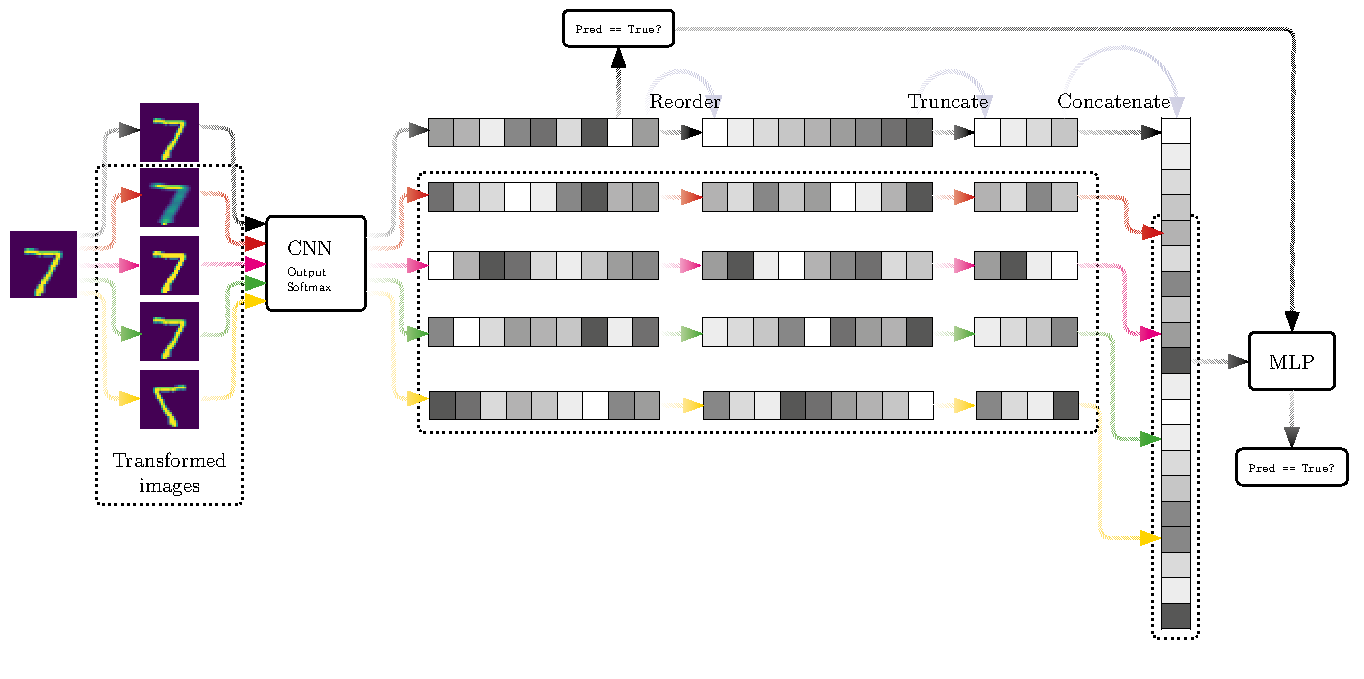
\includegraphics[width=\textwidth]{schema_baseline_1}
    \caption{Invariance To Image Transformation: Schema for \gls{MNIST} digit example \cite{Bahat_2018}.}
    \label{fig:schema-baseline1}
\end{figure}

This approach requires training an \gls{MLP} on top of an existing network to assess uncertainty, which can however be done efficiently and in time linear in the number of image transformations. A slightly more complex version of their algorithm for novelty detection has also been developed \cite{Bahat_2018}.

\subsubsection{MC-Dropout}
% MC-Dropout, uncertainty types
\textcite{ghahramani} propose the use of \gls{MC-Dropout} during prediction to quantify the model uncertainty. This method has been used as a de-facto uncertainty measure for neural networks in many papers \cite{mandelbaum17, leibig2017, Lakshminarayanan16, subramanya, Kampffmeyer2016SemanticSO}. In order for \gls{MC-Dropout} to work the neural network has to be trained with dropout applied after every convolution layer. Then, in order to retrieve the uncertainty $C(\mathbf{x})$ for a data point $\mathbf{x}$,  $T$ stochastic forward passes through the network are performed, each time randomly dropping a certain number of weights, thus only using a subset of all available weights for the prediction. The predictions are calculated as the average output of all $T$ runs and the certainty as the mean variance of the softmax outputs.


\subsection{Methods Based on Network Activations}
\label{subsec:pre-softmax}
As \textcite{ghahramani} point out, a model can be very uncertain about its predictions despite yielding a high softmax output. \textcite{NguyenYC14} demonstrate that neural networks can be easily fooled using an algorithm that generates images unrecognizable to humans but creating almost-100 per cent certainty predictions by the softmax activation output of the network. In addition, \textcite{Goodfellow2014} have shown that an adversary network can induce minor perturbations into an image, creating false predictions with very high confidence. Thus, many authors have decided to model the density of the network's pre-softmax activations of the training set for error detection and novelty detection tasks \cite{subramanya, mandelbaum17, Bishop1994NoveltyDA}.

\textcite{subramanya} point out that softmax scores can vary drastically when applying transformations such as Gaussian noise, blurring or JPEG compression to an image. In order to provide a more robust confidence estimator, they propose to model the density over each seen class in the pre-softmax activations: In order to estimate the confidence score of a prediction, they calculate the Gaussian densities belonging to the activations of the $N$ classes in a classification problem. Their confidence estimate yields more robust to image transformations such as noise injection and JPEG compression, but may suffer in case of Gaussian blurring and adversarial training.

\textcite{mandelbaum17} have opted for a similar approach, however approximating local density by the Euclidean distance between a point and its $k$ nearest neighbors in the embedded space created by the network in one of its pre-softmax layers. During test time, their method retrieves the activations of each data point and computes the distance to the $k$ nearest neighbors of each sample. In order to work, this method requires either adversarial training or a special loss function in which the distance between pairs of adjacent points belonging to different classes is maximized. Without this special loss function, their method yields worse or similar results compared to the baselines max margin and entropy \cite{mandelbaum17}. Using a modern \acrshort{GPU} implementation of nearest neighbor search, they achieve a computational complexity of $O(kN)$, $k$ being the number of nearest neighbors to search and $N$ the number of data points, making their method scale well with big datasets.

Other authors have proposed further similar variants of modelling the density or support of the pre-softmax activations \textcite{Bishop1994NoveltyDA}.

\subsection{Network Architectures for Confidence Estimation}
% Bayesian NNs
The current state-of-the art method to estimate uncertainty in \gls{ML} is based on \glspl{BNN}, allowing for direct estimation of the uncertainty from the model probabilities \cite{Gal2015Dropout,ghahramani,KendallG17}. However, this approach requires the network to be a Bayesian network, which implies changes such as optimizing over weight distributions instead of fixed weights. However, in \textcite{Gal2015Dropout, ghahramani}, the authors demonstrate the equivalence between a \gls{BNN} and a standard \gls{MLP} with dropout applied after every weight layer during test time (\gls{MC-Dropout}) with respect to confidence estimation.

% Adversarial training
\textcite{Goodfellow2014} show that adversarial examples can be used to improve the resistance of the network against \textit{fooling} attempts (sec. \ref{subsec:pre-softmax}), using \textit{Adversarial Training}. This however comes at a high price in computational cost at up to twice the training time \cite{mandelbaum17}.

% Deep Ensembles
Further methods have been developed based on \textit{ensembles} of NN models, such as in \textcite{Lakshminarayanan16, mandelbaum17}. These methods however suffer from heavily increased computation complexity for training several models.

\subsection{Comparison to Novelty Detection Methods}
% Novelty Detection overview
Many more novelty detection methods have been developed to model the support of data belonging to the ``normal'' class versus new ``anormal'' data \cite{Pimentel2014ARO, Markou2003NoveltyDApt1, Markou2003NoveltyDApt2}. They have been mainly characterized as probabilistic, distance-based, reconstruction-based and domain-based detection. Since not all methods could be implemented and evaluated, only a subset of the most popular novelty detection are covered. 

% Used methods
Two of the most common novelty detection methods are presented in this paper. The first are \glspl{GMM}, in which the assumption is made that the data was generated by an underlying mixture of Gaussian distributions \cite{Reynolds2009GaussianMM}. Some applications of \glspl{GMM} to novelty detection are presented in \cite{Pimentel2014ARO}. The second are \acrfullpl{OC-SVM}, in which the support boundary is searched for a given set of training points \cite{Wang2004AnomalyID, Beghi2014AOS}. \glspl{SVM} try to find a linear hyperplane using a kernel function, which can represent similarities between pairs of data points in an abstract geometric space \cite{Szymanski2011VisualisingKS}.

% TODO add illustration of GMM, OC-SVM
% Difference anomaly detection vs novelty detection
A difference between anomaly detection and novelty detection is that anomaly detection usually assumes novelties to be rare \cite{deMorsier2014thesis}. Some of the methods for anomaly detection include Isolation Forests and \gls{LOF} \cite{Pimentel2014ARO, Breunig2000LOFID, Liu2008IsolationF}. In contrast, \gls{GMM} and \gls{DF} can be seen as a clustering method, which require sufficient novelties to be available.

\subsection{Summary}
A summary of the reviewed literature and methods for confidence estimation in neural networks is given in table \ref{table:summary_literature}. Since the existing body of research on Confidence Estimation is vast and many related papers exist to each of the presented topics, only a selection of reviewed papers is presented.

\begin{table}[H]
    \centering
    \small
    \begin{tabular}{llll}
    \toprule
        Type & Reference & Method & Focus \\\midrule
         \multirow{4}{*}{\shortstack[l]{Softmax\\ scores}} &\textcite{HendrycksG16c} & \textbf{MSR, Margin, Entropy} & Softmax activations \\
         &\textcite{Bahat_2018} & \textit{Tranformations Invariance} & Data Perturbations  \\
         &\textcite{ghahramani} & \textbf{\gls{MC-Dropout}} & Model Perturbations \\
         &\textcite{Sun2018KSconfA} & \textbf{\gls{KS}-Test} & \gls{KS}-test on softmax output \\\midrule
         \multirow{2}{*}{\shortstack[l]{Pre-softmax\\ activations}}&\textcite{subramanya}& \textit{Density} & Density Modelling\\
         &\textcite{mandelbaum17}& \textit{Distance} & \textit{k-nn} Distance\\\midrule
         \multirow{3}{*}{\shortstack[l]{New Network\\ Architectures}}&\textcite{Goodfellow2014} & \textit{Adversarial Training} & Training Perturbations\\
         &\textcite{KendallG17} & \textit{\glspl{BNN}} & Bayesian Neural Networks \\
         &\textcite{mandelbaum17} & \textit{Ensembles} & Neural Network Ensembles \\
         \bottomrule
    \end{tabular} 
    \caption{Summary of reviewed confidence measures for neural networks. Implemented baselines are indicated in bold.}
    \label{table:summary_literature}
\end{table}

In addition to the implemented baselines indicated in bold in table \ref{table:summary_literature}, Novelty Detection methods \textit{GMMs} and \textit{OC-SVMs} have been implemented to detect novelties from the network activations.

\section{Methodology}

\subsection{Overview: \acrlongpl{DF}}
% Introduction
Similar to the activations-based methods presented in section \ref{subsec:pre-softmax}, the confidence measure developed below tries to distinguish activations of the training set from new, unseen activations in the test set. Similar to the way Decision Trees and Random Forests are used in the case of labelled data, Density Trees and \acrlongpl{DF} are used for unlabelled data to distinguish ``normal'', seen data from unseen, new data points.

% Decision Trees
The methodology proposed below is based on previous work by \textcite{decisionForests-MSR}, who propose a unified framework for random decision forests, which can be extended to classification, regression, density estimation and other tasks. Therefore, this unifying framework of decision forests is first addressed before covering the extension to \acrlongpl{DF}.

% Structure
This section is structured as follows: First, the developed method for assessing uncertainty is presented. Second, evaluation schemes for all experiments are discussed. Last, the hyperparameter search scheme for \acrlongpl{DF} is discussed.

% Schema
An overview of the methodology for novelty detection using \acrlongpl{DF} is shown in figure \ref{fig:schema}.

\begin{figure}[H]
    \centering
    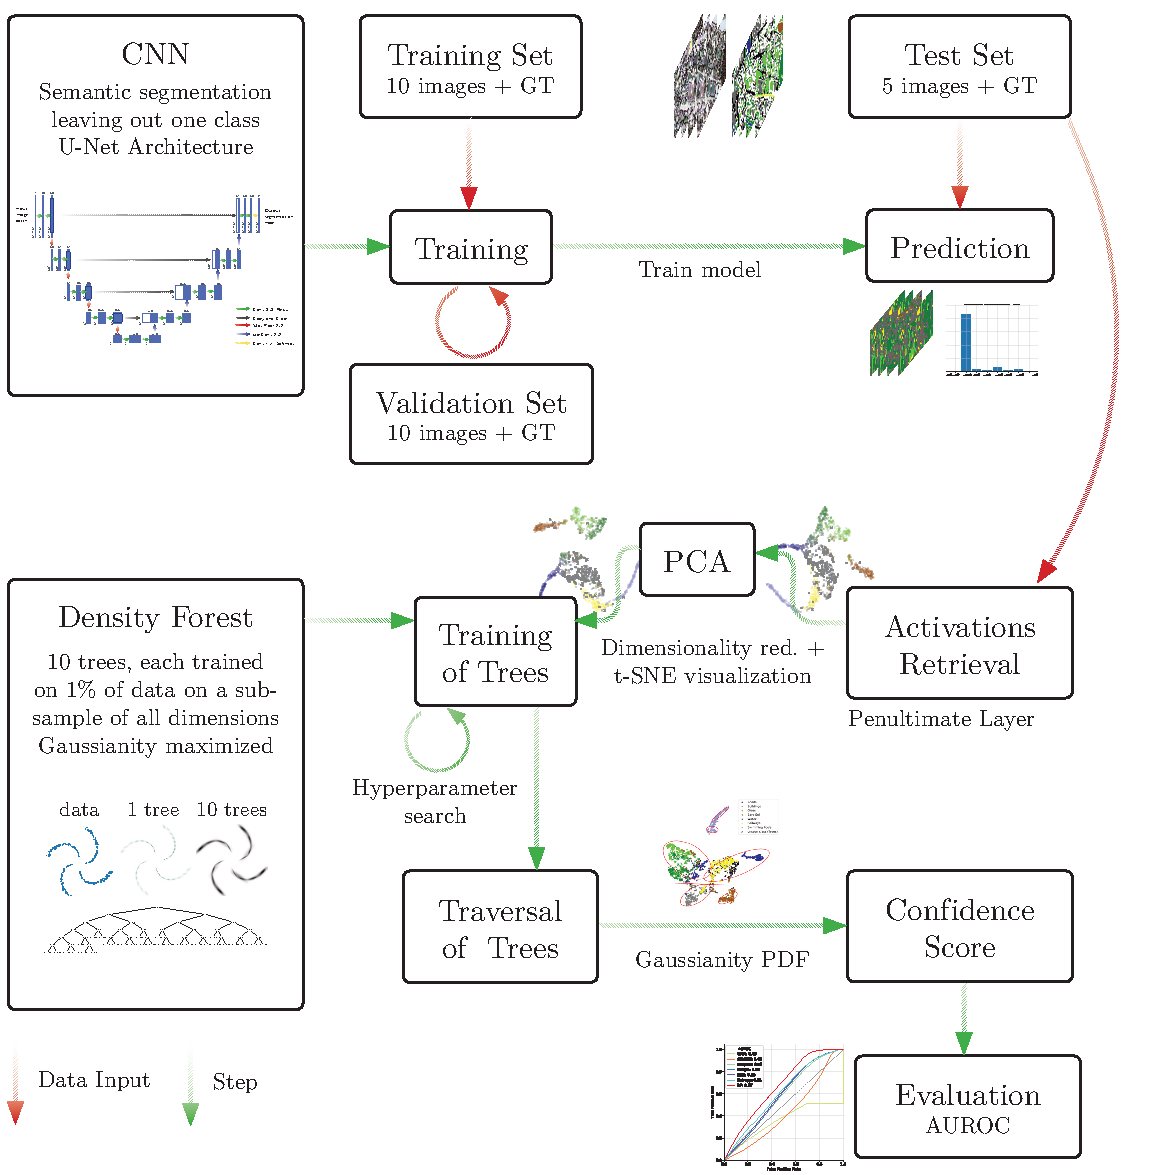
\includegraphics[width=\textwidth]{schema_df}
    \caption{Workflow Diagram}
    \label{fig:schema}
\end{figure}

\subsection{Decision Trees}
% Introduction
A Decision Tree is a binary tree consisting of hierarchical nodes and edges which, at each level, provide the most important features to determine the outcome of a dependent variable, given an arbitrary number of independent variables \cite{decisionForests-MSR}. At each level starting from top to bottom, the goal of a Decision Tree is to find the best possible split to partition the feature space $S$ such as to minimize an entropy function $H(S)$ in every subdomain. At every splitting step, an \acrlong{IG} function is maximized:

% Information gain
\begin{equation}
    \label{eq:ig}
    I = H(\mathcal{S})-\sum_{i\in \{l,r\}}\frac{|\mathcal{S}_i|}{|\mathcal{S}|}H(\mathcal{S}_i)
\end{equation}
Where $I$ is the \acrlong{IG}, $H$ is an optimizer or entropy function, $S$ is the original dataset at a node and $S_i$ is left and right data subset resulting from the split.

% Entropy
For instance, in the case of labelled data and decision forests, the Shannon entropy is often used:
\begin{equation}
    H(\mathcal{S}) = -\sum_{c\in\mathcal{C}}P^{(c)}\log(P^{(c)})
\end{equation}
$P^{(c)}$ being the probability of an outcome $c$ for a discrete random variable with possible outcomes $\mathcal{C}$. Within each dimension, a range of possible split values is checked to find the split which minimizes entropy, i.e., maximizing information gain. For each candidate split dimension, a number of candidate split values have been tested randomly between the interval of the $dim$-th smallest and $dim$-th largest data point values, such as to ensure at least $dim$ datapoints to either side of the split to ensure inversible matrices.

% Stopping Criteria
Stopping criteria for growing individual tree branches have been implemented according to \cite{decisionForests-MSR}, based on maximum maximum tree depth and based on the minimum Information Gain required at each node to continue splitting. The implemented data structure of a Decision Tree node is represented in appendix \ref{subsec:implementation}.

\subsection{Random Forests}
% Random Forests
Smoother and more generalized boundaries can be obtained by using Random Forests, which combine a set of individually trained trees on bootstrapped subsamples of the initial data \cite{decisionForests-MSR, Breiman2001}. Bootstrapping is a technique of sampling a smaller subset of data from a larger subset with replacement \cite{Zoubir2007BootstrapMA}. The aggregation of multiple predictors based on bootstrapped samples is usually referred to as bagging \cite{Breiman1996BaggingP}. A simple visualization of Random Forests on generated synthetic data is provided in appendix \ref{app:rf}. Aside of the parameters and stopping criteria mentioned for individual trees, important factors for Random Forests are the number of trees, the subsample size of the initial data on which each tree is trained and the number of dimensions each node may consider as a candidate dimension for splitting.

\subsection{\acrlongpl{DF}}

% Information Gain, Entropy
A Density Tree can be seen as similar to Decision Trees, but with the aim of clustering \textit{unlabelled} data into regions that maximize the Gaussianity of each cluster \cite{CW2017}. Same as with Decision Trees, a generic information gain function is maximized (eq. \ref{eq:ig}). An unsupervised entropy function is designed based on the assumption of a multivariate Gaussian distribution at each tree node \cite{decisionForests-MSR}:

\begin{equation}
    H(\mathcal{S}) = \frac{1}{2}\log\Big((2\pi e)^d|\mathtt{\Lambda}(\mathcal{S})|\Big)
\end{equation}
$\mathtt{\Lambda}$ being the associated $d \times d$ covariance matrix. Hence, the information gain at the $j^{\text{th}}$ split becomes \cite{decisionForests-MSR}:
\begin{equation}
    I_j = \log(|\mathtt{\Lambda}(\mathcal{S}_j)|) - \sum_{i\in \{l, r\}}\frac{|\mathcal{S}_j^i|}{|\mathcal{S}_j|}\log(|\mathtt{\Lambda}(\mathcal{S}_j)|)
\end{equation}

For a description of the motivation behind this optimization method, refer to \cite{decisionForests-MSR}. The implemented data structure for Density Trees is represented in in appendix \ref{subsec:implementation}.

% Prediction
At prediction time, a given data point descends the Density Tree according to the split dimension and value associated with each tree node until it reaches a leaf node. The probability of the data point to belong to a cluster of the tree is calculated with respect the leaf node cluster \cite{decisionForests-MSR}:
\begin{equation}
    \label{eq:proba_density}
    p_t(\mathbf{x}) = \pi_l\mathcal{N}(\mathbf{x}|\boldsymbol{\mu}_{l(\mathbf{x})},\mathtt{\Lambda}_{l(\mathbf{x})})
\end{equation}
With $\boldsymbol{\mu}_{l(\mathbf{x})}$ and $\mathtt{\Lambda}_{l(\mathbf{x})}$ denoting the mean and covariance of the leaf node corresponding to the data point $\mathbf{x}$, $\pi_l$ being the proportion of points falling into the respective leaf node. The multivariate Gaussian \acrfull{PDF} is defined as follows:
\begin{equation}
    \label{eq:mv-gaussian}
    \mathcal{N}(\mathbf{x}|\boldsymbol{\mu},\mathtt{\Lambda})=\frac{1}{\sqrt{(2\pi)^k\det\mathtt{\Lambda}}}\exp\Big({-\frac{1}{2}(\mathbf{x}-\boldsymbol{\mu}})^\top\mathtt{\Lambda}^{-1}(\mathbf{x}-\boldsymbol{\mu})\Big)
\end{equation}
Where $\boldsymbol{\mu}$ is the mean, $\mathtt{\Lambda}$ is the co-variance matrix and $k$ is the number of dimensions of $\mathbf{x}$ \cite{scipy}. The thus obtained probability is weighted by the percentage $\pi_l$ of all the data used for training the Density Tree falling into this leaf node. For the purpose of this study, a simple \acrlong{DF} without the probability normalization term $Z_t$ was implemented. However, for comparisons between several models, the output probabilities would need to be normalized by a partition function $Z_t$ as in equation \ref{eq:proba_density}.

Figure \ref{fig:DF-split-visu} illustrates the splitting steps for a single Density Tree. 

\begin{figure}[H]
	\centering
	% loop classes
	\foreach \i in {1,...,3}
	{
		\begin{subfigure}{.3\textwidth}
			\centering
			\includegraphics[width=\textwidth]{Schema/df-step\i}
			\includegraphics[width=\textwidth]{Schema/df-step\i-tree}
			\caption{Step \i}
		\end{subfigure}
	}\\
	\foreach \i in {4,5}
	{
		\begin{subfigure}{.3\textwidth}
			\centering
			\includegraphics[width=\textwidth]{df-step\i}
			\includegraphics[width=\textwidth]{df-step\i-tree}
			\caption{Step \i}
		\end{subfigure}
	}
	\caption{Illustration of tree growth for a fictive dataset. Covariance ellipses are indicated in red lines and splitting lines in red dotted lines, indicating the dimension and value along which a node is split. Nodes are considered leaf nodes when no further split is necessary or possible, either because the Information Gain of a new split would be too low or because the maximum depth is reached. In a \acrlong{DF}, every tree would gets to see a subset of all points and fit slightly different leaf nodes.}
	\label{fig:DF-split-visu}
\end{figure}


At every step of the Density Tree creation, splits are created such as to maximize the Gaussianity on either side of the node. The maximum number of splits can either be based on an Gaussianity criterion, maximum tree depth or be fixed to an arbitrary number. Parameters for \acrlong{DF} are listed in table \ref{table:df-parameters}.

\begin{table}[H]
    \centering
    \begin{tabular}{p{3cm}p{9cm}p{2.5cm}}
    \toprule
    Parameter & Description & Range \\ \midrule
    \texttt{n\_trees} & Number of trees created. A higher number of trees increases training and prediction time by a linear amount. & 10 - 50 \\
    \texttt{subsample\_pct} & Size of each random data subset sampled from the original dataset used as input for a Density Tree, in percentage of the size of the original dataset & 0 - 0.1 \\
    \texttt{max\_depth} & Maximum depth allowed for each tree. Improves generalization ability of individual trees. & 4 - 20 \\
    \texttt{min\_subset} & Minimum subset of each data to be contained in each cluster, as percentage of the subsample dataset size. & 2 - 3 $\times$ \texttt{dim} \\
    \texttt{n\_max\_dim} & Number of dimensions to consider for splitting at each node. If \texttt{dim} $\leq 0$, all dimensions are considered. If \texttt{dim} $> 0$, a random number of dimensions between 1 and dim is considered for splitting at each node. Increases speed and further adds randomization to trees. & 0 - \texttt{dim} \\
    \texttt{ig\_improvement} & The Information Gain improvement that has to be made at each node in order to create a new split. Avoids unnecessary splits in already Gaussian clusters & 0 - 0.9\\\bottomrule
    \end{tabular}
    \caption{\acrlong{DF} parameters and suggested parameter ranges}
    \label{table:df-parameters}
\end{table}


\section{Datasets}
% Overview

\subsection{Synthetic Datasets}
\label{subsec:data-synthetic}
% Synthetic Data
First, some synthetic data was produced to test how well individual Density Trees could fit points generated in 2-dimensional space, and visualize the found decision boundaries. The following three data generators were used:
\begin{enumerate}
    \item A generator which produces $n$ clusters according to Gaussian distributions $\mathcal{N}(\mathbf{x}|\boldsymbol{\mu},\mathtt{\Lambda})$ with fixed parameters $\boldsymbol{\mu},\mathtt{\Lambda}$. For each cluster, the covariance ellipses can be randomly multiplied by a coefficient in one dimension, such as to create an elongated cluster, and non-linear transformations can be applied randomly.
    \item A spiral data generator, which produces points along a spiral, with the points $x$ and $y$ being generated as:
    \begin{equation}
        \begin{aligned}
            x &= a\sqrt{\theta}\cos\theta\\
            y &= a\sqrt{\theta}\sin\theta
        \end{aligned}
    \end{equation}
    $\theta$  being the angle and $a$ being the distance between successive terms of the spiral.
    \item A generator which produces data along an S shape similar to the method above, but with only one arm, generating data points as follows:
    \begin{equation}
        \begin{aligned}
            x &= a\sqrt{\theta}\sin\theta\\
            y &= xa\sqrt{\theta}\sin\theta
        \end{aligned}
    \end{equation}
\end{enumerate}

Datasets generated according to these three data generators are shown in figure \ref{fig:synthetic-datasets}.

\begin{figure}[H]
    \begin{subfigure}{.38\textwidth}
        \centering
        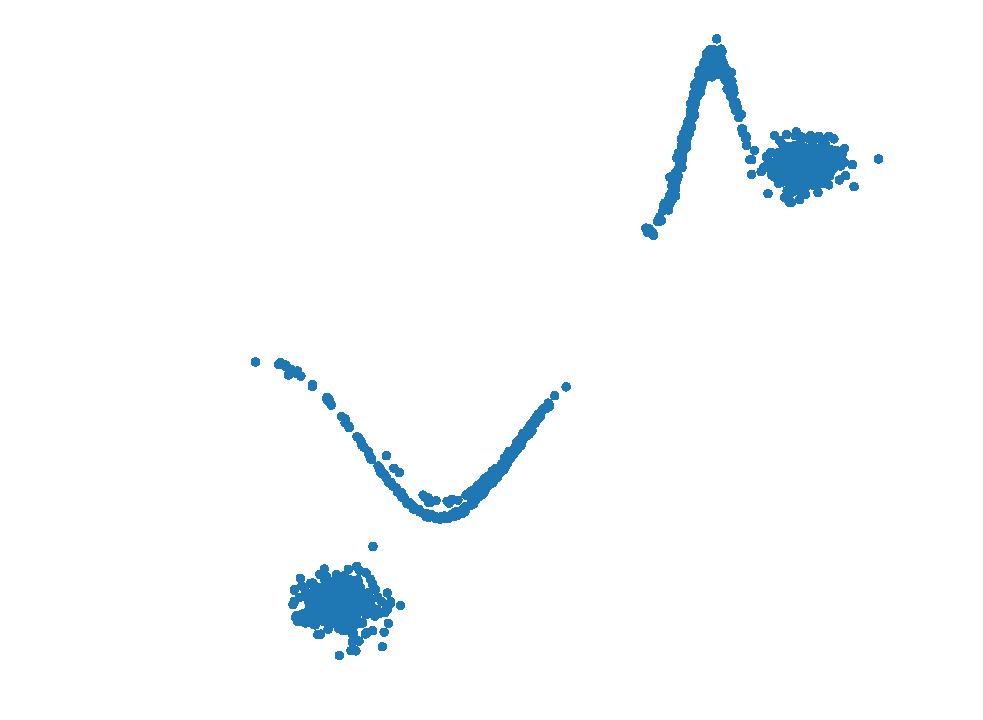
\includegraphics[width=\textwidth]{D1_data}
        \caption{4 clusters with transformations}
    \end{subfigure}
    \begin{subfigure}{.3\textwidth}
        \centering
        
\includegraphics[width=\textwidth]{D2_data}
        \caption{Spiral with 4 arms}
    \end{subfigure}
    \begin{subfigure}{.3\textwidth}
        \centering
        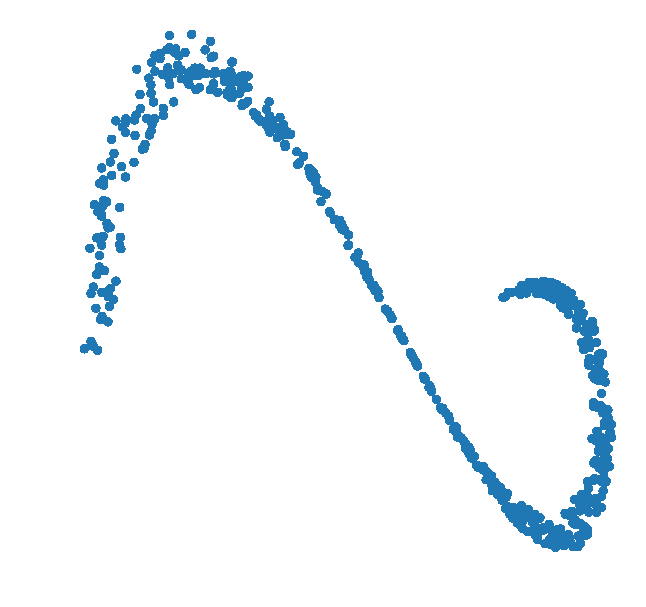
\includegraphics[width=\textwidth]{D3_data}
        \caption{S-shaped distribution}
    \end{subfigure}
    \caption{Synthetic datasets}
    \label{fig:synthetic-datasets}
\end{figure}

% \gls{MNIST}
\subsection{\gls{MNIST} Dataset}
Confidence Measures have been first applied to the \gls{MNIST} dataset, containing 24 $\times$ 24 gray level images of handwritten digits from 0 to 9 and corresponding labels \cite{mnist}. The training set and test set consist of 60'000 and 10'000 samples respectively, with roughly the same amount of images for each class. Some examples of handwritten digits are shown in figure \ref{fig:MNIST-Im}.

% MNIST images
\begin{figure}[H]
    \centering
    % loop rows
    \foreach \j in {0,...,2}
        {
        % loop classes
        \foreach \i in {0,...,9}
        {
        \begin{subfigure}{.08\textwidth}
            \centering
            \includegraphics[width=\textwidth]{MNIST_cl_\i_\j}
        \end{subfigure}
        }
        \\
    }
    \caption{Sample images of the \gls{MNIST} dataset for true y labels 0 to 9 \cite{mnist}}
    \label{fig:MNIST-Im}
\end{figure}

\subsection{Zurich Dataset}
\label{subsec:data-zurich}
% Dataset
In addition to confidence estimation on synthetic data and the \gls{MNIST} dataset, the confidence measures were applied to semantic segmentation, which consists of attributing a class label to every pixel of an image \cite{Volpi2017DenseSL}. For this task, the ``Zurich Summer v1.0'' (Zurich) dataset was used, consisting of a set of 20 RGB-IR satellite images taken from a QuickBird acquisition of the city of Zurich (Switzerland) in August 2002, together with a corresponding set of annotated ground truth images \cite{Volpi2015SemanticSO}. 8 different urban and peri-urban cases have been annotated: Roads, Buildings, Trees, Grass, Bare Soil, Water, Railways and Swimming Pools. The Zurich dataset was split into a training set consisting of images 1-10, a validation set consisting of images 11-15 and a test set consisting of images 16-20, corresponding roughly to a 50/25/25 split. An example pair of an RGB-IR image and its ground truth is given in fig. \ref{fig:zh-im-gt-pair}.

\begin{figure}[H]
    \centering
        \begin{subfigure}{0.41\textwidth}
            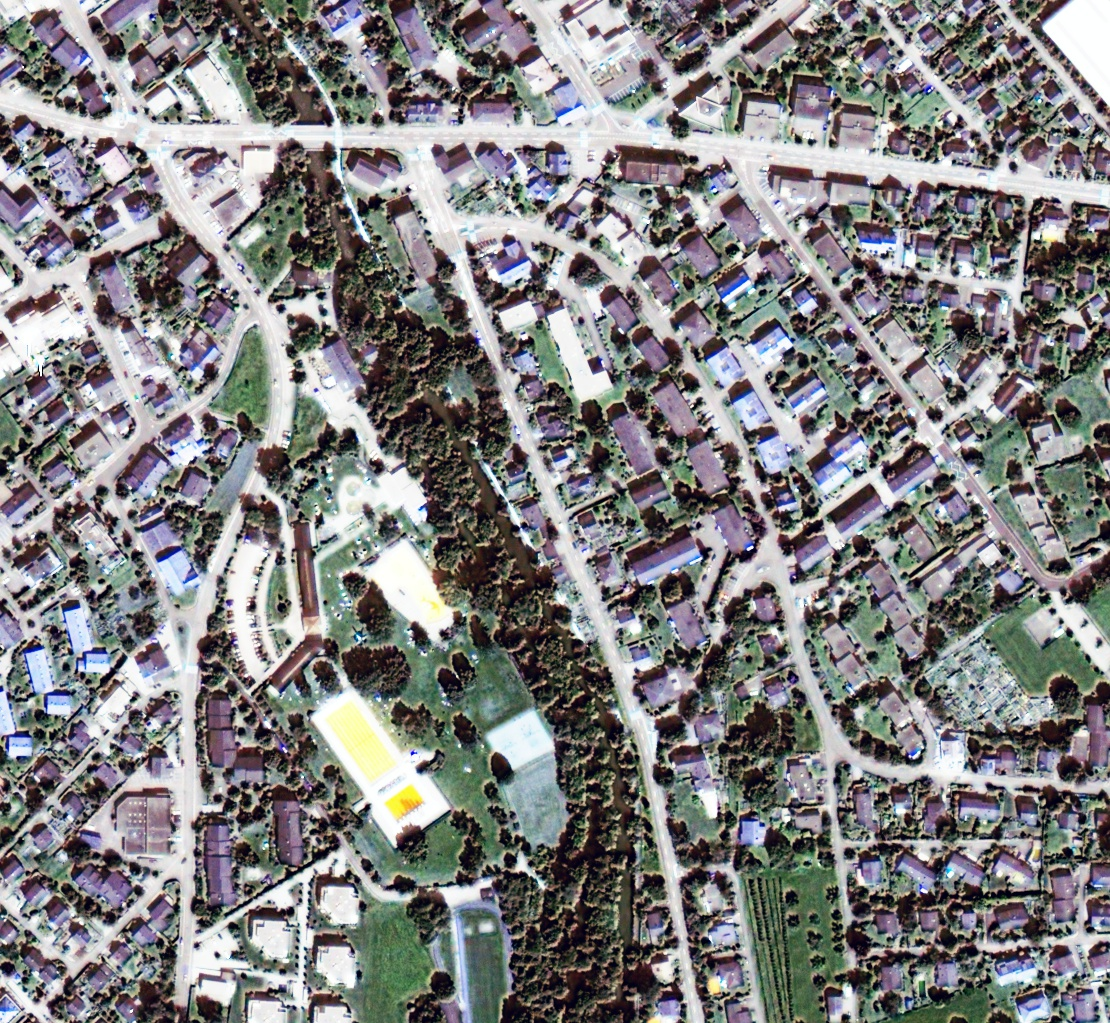
\includegraphics[width=\textwidth]{Im_16}
            \caption{RGB-IR image}
        \end{subfigure}
        \begin{subfigure}{0.41\textwidth}
            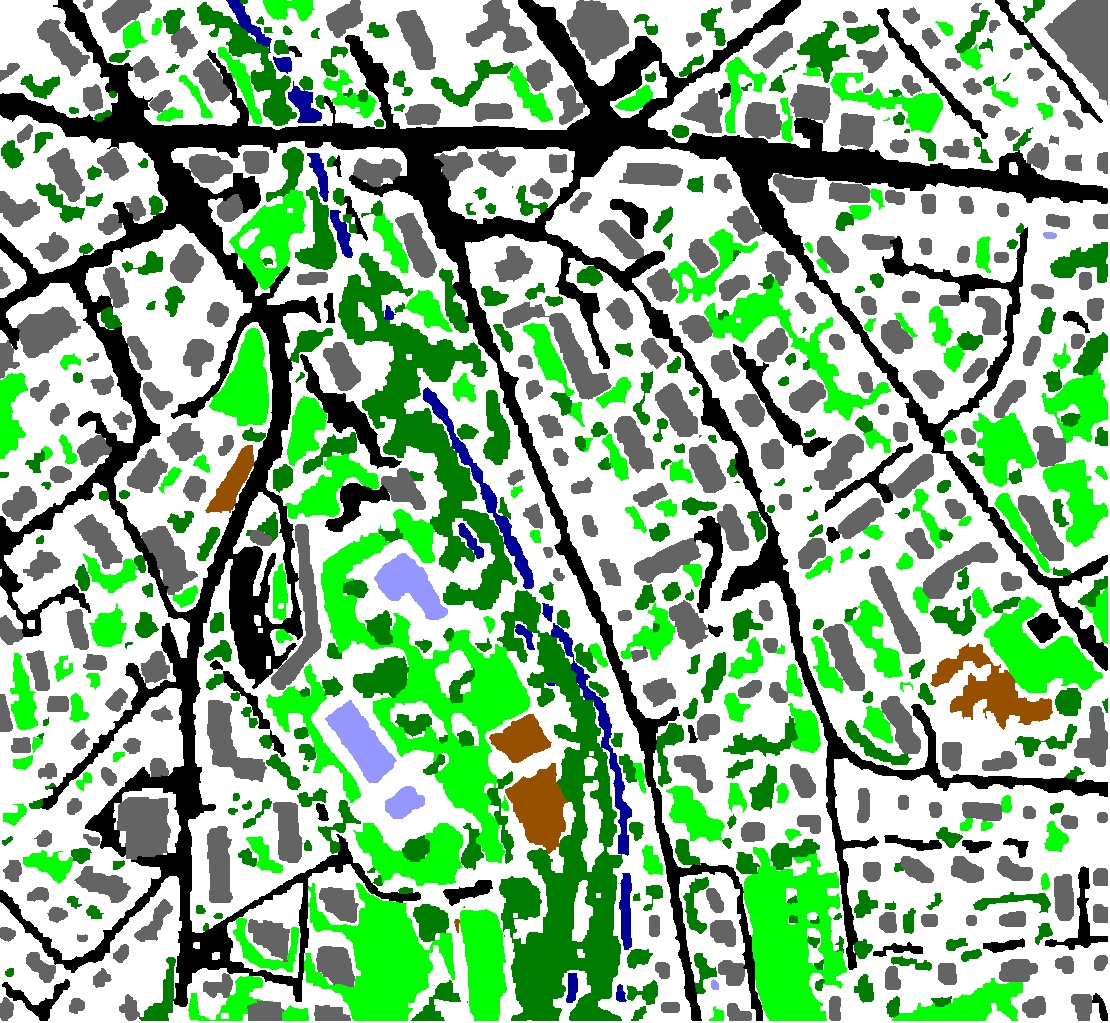
\includegraphics[width=\textwidth]{GT_16}
            \caption{Ground truth}
        \end{subfigure}
    \\[.2cm]
    \legendH
    \caption{Sample pair of images and ground truth for the Zurich dataset \cite{Volpi2015SemanticSO}}
    \label{fig:zh-im-gt-pair}
\end{figure}

% Class imbalance
Classes are imbalanced, with only very few samples for some classes, such as swimming pools or railways (fig. \ref{fig:label-dist-zurich}).

\begin{figure}[H]
    \centering
    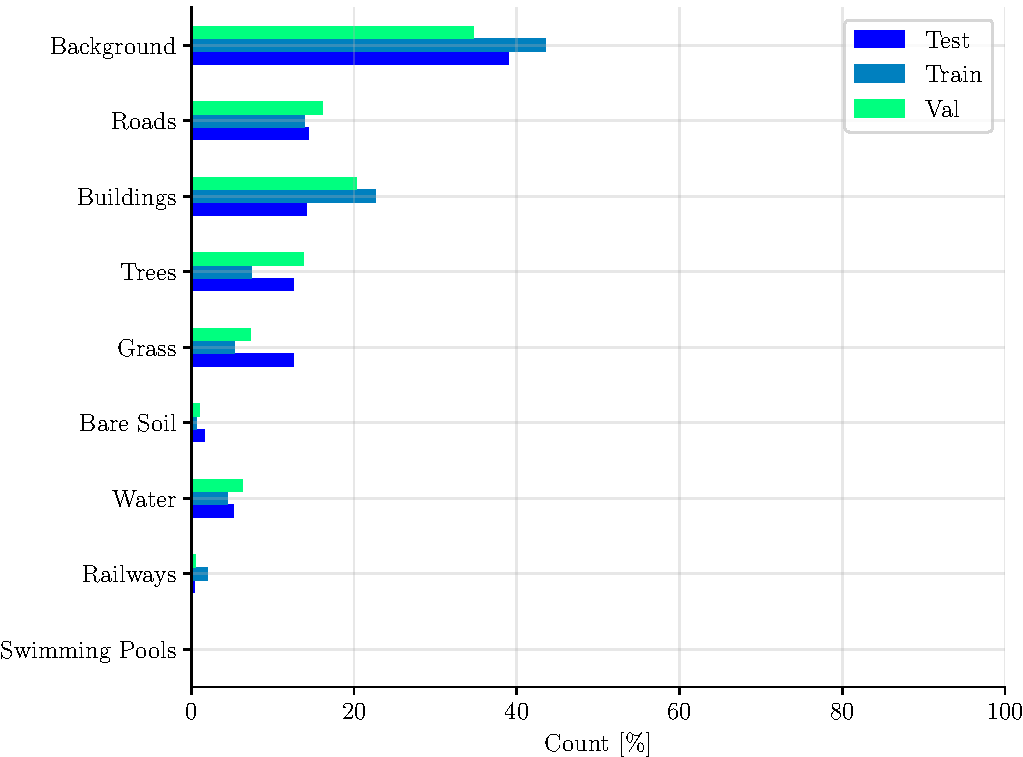
\includegraphics[width=.7\textwidth]{ZH_dist}
    \caption{Label distribution in the Zurich dataset}
    \label{fig:label-dist-zurich}
\end{figure}


\section{Experimental Setup}
\label{sec:experimental-setup}
\subsection{Network Architectures}
\label{sec:network-architectures}
% MNIST dataset
% Training / Testing split, leave-one-out
\paragraph{\gls{MNIST} dataset} The original \gls{MNIST} dataset consists of a training set of 60'000 images and a test set of 10'000 images, both containing a roughly equal amount of images belonging to the labels 0-9 \cite{mnist}. 10 \gls{CNN} models were each trained on about 45'000 training images, removing images of the left-out class, and validated on 10'000 test images, including images of the left-out class.

% Network architecture
\glspl{CNN} were trained both for novelty detection using the network architecture described in table \ref{table:CNN_MNIST}. For novelty detection, \glspl{CNN} have been trained leaving out each time one class. Dropout was added after each MaxPooling layer to increase the redundancy of the network and avoid overfitting \cite{Srivastava2014DropoutAS}. The \gls{ReLU} activation function ($f(x) = \max(0, x)$) was used after each convolution layer of the network.  The \gls{FC} layer denotes the pre-classification layer in the network, in which every input is connected to every output by a weight and followed by a \gls{ReLU} activation.

\begin{table}[H]
    \begin{center}
    \begin{tabular}{ll}
    \toprule
    Layer & Properties \\
    \hline
    Input & Dimension $|b| \times 28 \times 28$ \\ 
    Convolution + \gls{ReLU} & 32 3 $\times$ 3 filters\\
    Convolution + \gls{ReLU} & 64 3 $\times$ 3 filters\\
    MaxPooling & 2 $\times$ 2 pool size \\
    Dropout & $p = 0.25$ \\
    \hline
    Flatten & \\
    Dense (\gls{FC}) + \gls{ReLU} & 128 neurons\\
    Dropout & $p = 0.5$ \\
    Output + Softmax & 9 neurons \\
    \bottomrule
    \end{tabular}
    \caption{Architecture of the \gls{CNN} used for \gls{MNIST} digit classification. $|b|$ = batch size, $p$ = dropout probability.}
    \label{table:CNN_MNIST}
    \end{center}
\end{table}

\paragraph{Zurich dataset} Similar as for the \gls{MNIST} dataset, \gls{CNN} models were trained for each left-out class. The U-Net network architecture shown in figure \ref{fig:u-net} was applied to perform semantic segmentation on the Zurich dataset. It consists of a sequence of down-sampling and up-sampling layers, yielding a ``U''-shaped layer architecture \cite{ronneberger2015u}. This architecture has shown good performance in various semantic segmentation tasks, and has been especially applied in medical imaging \cite{ronneberger2015u, Alom2018RecurrentRC, Dong2017AutomaticBT}. A full overview of the layers is given in appendix table  \ref{table:CNN_Zurich}.

\begin{figure}[H]
    \centering
    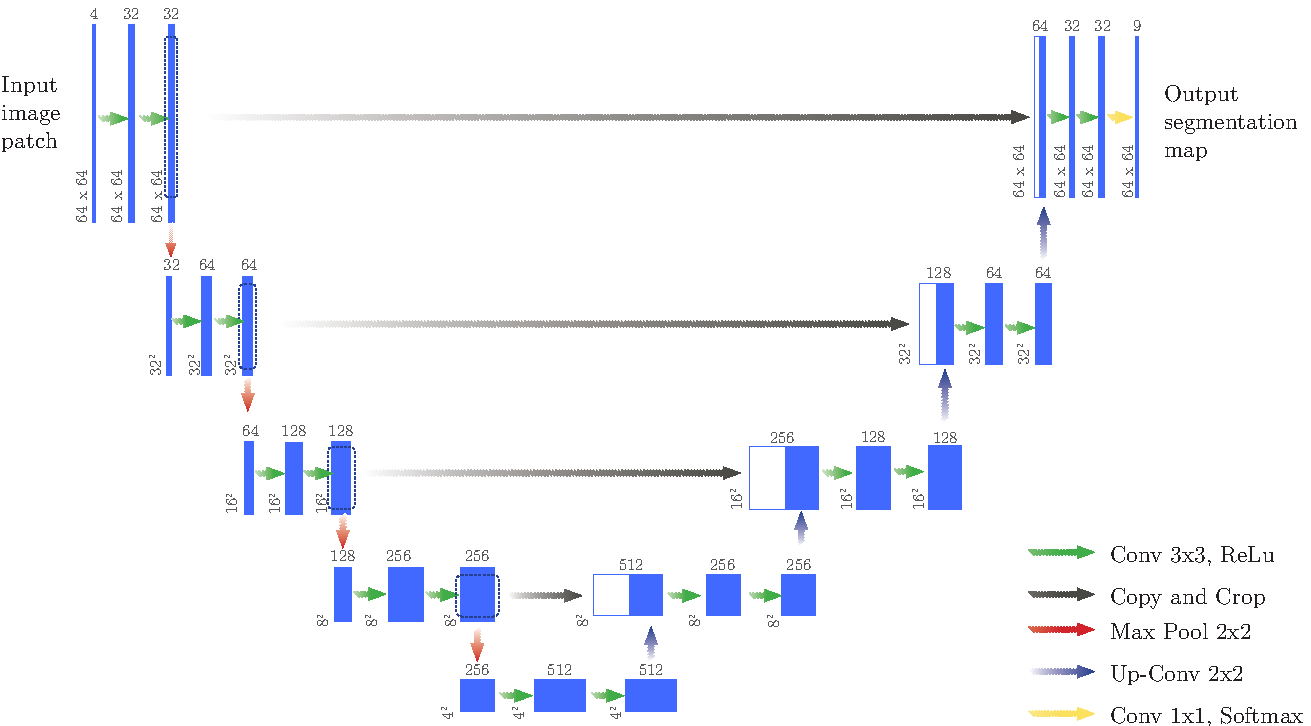
\includegraphics[width=\textwidth]{unet}
    \caption{U-Net architecture, according to \textcite{ronneberger2015u}}
    \label{fig:u-net}
\end{figure}
% Image tiling
For training the U-Net model, the training and validation images were tiled into \textit{non-overlapping} patches of patch size size $64 \times 64 \times n_c$ where $n_c$ is the number of channels. For prediction, the test set images were tiled into \textit{overlapping} patches using the same patch size of size $64 \times 64 \times n_c$, with several different strides between patches, keeping only the central overlapping \textit{stride $\times$ stride} pixels between adjacent patches. Central pixels of a patch are assumed more certain because of the larger available spatial context in the patch compared to pixels near the patch borders which partially lack neighbor information, leading to strong border effects \cite{Marmanis2016SemanticSO}. Although the optimal stride would seem to be 1, keeping only the central pixel would lead to excessive computational costs with little additional accuracy gain. Therefore, intermediate strides have to be chosen empirically. For a given stride and patch size, the image was first padded on each side to make it divisible by \textit{stride}, and by an additional amount \textit{(patch size - stride) / 2} on either side of the image to be able to fit patches of size $64 \times 64$ with the given stride around the entire padded image. For each patch, only the $stride \times stride$ central pixels were kept and any remaining pad was removed from the image to give it the same dimensions as the input image. Several strides were chosen and results averaged to further reduce border effects. For instance, for a stride of 32 pixels and a patch size of 64 pixels, patches of $64 \times 64 \times n_c$ are created and only the $32 \times 32 \times n_c$ central pixels are kept for the final prediction (fig. \ref{fig:im_padding}).



% Padding figure
\begin{figure}[H]
    \centering
    \includegraphics[width=.5\textwidth]{im_padding}
    \caption{Padded image and patches for a given patch size and stride. The big blue rectangle delimits the image area outside of which the original image is padded using mirroring. The rainbow-colored rectangles show patches with an overlap between pairs of patches defined by the stride. The central $stride \times stride$ solid-filled rectangles within each patch show the patch areas which are kept after prediction. The red dotted line shows the size of the image that is obtained after merging all predictions within the central areas of the patches. Finally, the thus obtained prediction image is cropped to the big blue box, denoting the original image size. Final predictions are obtained using several strides and averaging the results.}
    \label{fig:im_padding}
\end{figure}

% Data augmentation
Data augmentation was performed to improve the accuracy of the network. Following transformations have been applied both to the image and ground truth patches, according to \textcite{Volpi2017DenseSL}:
\begin{enumerate}
    \item Extraction of patches at random locations of the training set images to avoid seeing the same types of patches in each training minibatch. Class imbalance is not considered during patch extraction.
    \item Random horizontal and vertical flipping and random rotations in steps of 90 degrees (0, 90, 180 or 270 degrees). These transformations aim at improving invariance to differing spatial organizations of the image.
    \item Noise injection: Add noise to every pixel of the image, sampling the noise from a Normal distribution in $\mathcal{N}(0, 0.01)$, scaling the input data in $[0, 1]$
\end{enumerate}

\subsection{Novelty Detection Baselines}
Some implementation details are discussed below for other novelty detection baselines to which \acrlongpl{DF} are compared. 

% Network methods
\paragraph{MSR, Margin, Entropy} The confidence measures relying on the softmax output of a network which were implemented using the equations of section \ref{sec:lit} (eq. \ref{eq:net_msr}, \ref{eq:net_margin} and \ref{eq:net_entropy})

% Implemented MC-Dropout method
\paragraph{MC-Dropout} In this study, a slightly simplified version of the \gls{MC-Dropout} algorithm was implemented, performing dropout during test time only in the \gls{FC} pre-softmax layer and calculating the entropy (eq. \ref{eq:net_entropy}) on the mean of the softmax activations. This has the advantage of speeding up calculations by having to repeat only the pass through the last layers of the network instead of the entire pass.

% GMM, OC-SVM
\paragraph{Pre-softmax methods} In this work, the \gls{GMM} and \gls{OC-SVM} approaches have been applied to novelty detection using the same activations to find the support of the ``normally distributed'' data as the \acrlong{DF}. For both \gls{GMM} and \gls{OC-SVM}, the Scikit-learn implementations were used \cite{scikit-learn}.  As confidence values, \gls{GMM} calculates the log-likelihood for a given a data point and \gls{OC-SVM} calculates the signed distance from the separating hyperplane, being positive for inliers and negative for outliers.

\subsection{Dimensionality Reduction and Data Separability}
\label{subsec:methodology-dim-reduction}
For both the \gls{MNIST} dataset and the Zurich dataset, activations were retrieved for training and descending Density Trees, which results in a large number of input dimensions. For example, the \gls{FC} layer of the \gls{MNIST} dataset contains 128 filters, therefore, for a batch $n$ images, the activation weights retrieved during prediction are of dimension $n \times 128$ (table \ref{table:CNN_MNIST}). Many of these activations are similar, which causes collinearity and matrix inversion issues during the calculation of the Gaussian entropy. Therefore, a dimensionality reduction was performed using \acrfull{PCA}. For \gls{MNIST}, the 15 first components were kept, explaining about 70-80 \% (fig. \ref{fig:pca_components}). For the Zurich dataset, the first 5 dimensions were kept, explaining about 90-95 \% of the data variance. The choice not to exceed 15 components for the \gls{MNIST} set was made to limit the already high computation complexity for Gaussianity estimation. Another reason to prefer low-dimensional data is to avoid the curse of dimensionality, which causes notions of distance between points to become meaningless and which, together with data noise, negatively impacts performance of many clustering algorithms \cite{Hinneburg2000WhatIT, Hinneburg1999OptimalGT}. \\

\begin{figure}[H]
    \centering
    \begin{subfigure}{.45\textwidth}
        \centering
        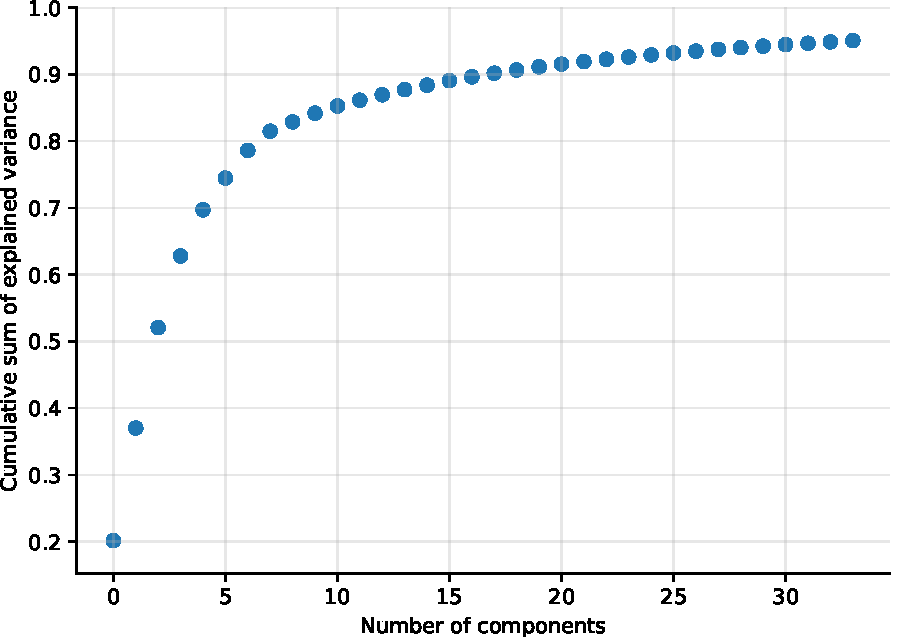
\includegraphics[width=\textwidth]{MNIST_pca_components_wo_cl_8}
        \caption{\gls{MNIST} dataset, left-out class 8}
        \label{fig:pca_components_mnist}
    \end{subfigure}
    \begin{subfigure}{.45\textwidth}
        \centering
        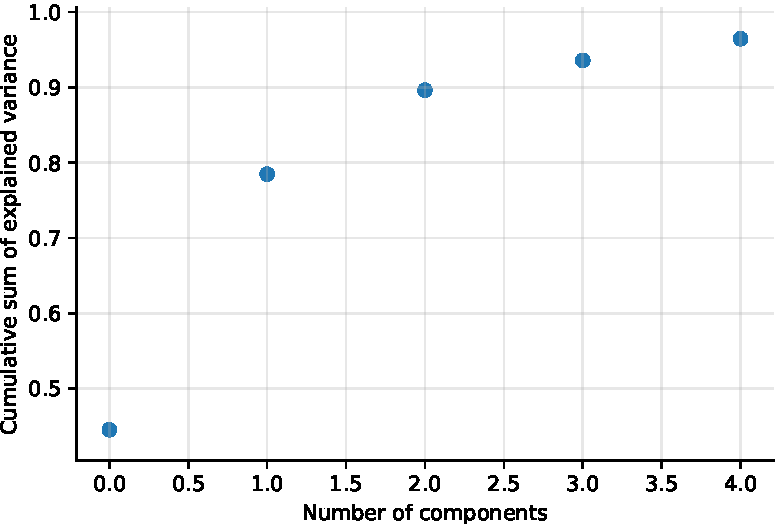
\includegraphics[width=\textwidth]{ZH_pca_components_wo_cl_1}
        \caption{Zurich dataset, left-out class roads}
        \label{fig:pca_components_zurich}
    \end{subfigure}
    \caption{Explained variance as a function of the number of components}
    \label{fig:pca_components}
\end{figure}
% t-SNE
Separability between activations corresponding to different classes was ensured before and after \gls{PCA}, using \acrfull{t-SNE} for visualization of high-dimensional data \cite{Maaten2008VisualizingDU}. \gls{t-SNE} tries to find a mapping between high-dimensional data points and their representation in a lower-dimensional space, typically in 2 to 3 dimensions, by preserving the local structure of the original, high-dimensional data (fig. \ref{fig:t-SNE-schema}). To preserve the original data structure, \gls{t-SNE} models the pairwise similarity between data points in their high-dimensional and lower-dimensional space. Similarities between pairs of data points $x_j$ and $x_i$ are measured as the conditional probabilities of $x_i$ choosing $x_j$ as its neighbor, if neighbors were picked in proportion to their probability density of a Gaussian centered at $x_i$ \cite{Maaten2008VisualizingDU}. \gls{t-SNE} uses a cost function to minimize the sum of Kullback-Leibler divergences over all data points, measuring the differences between similarity values in higher and lower dimensions. Since \gls{t-SNE} directly transforms the training data without finding a parametric mapping, it can only be applied to the training data. This makes it hard to apply the t-SNE to all activations due to increased training times.


\begin{figure}[H]
	\centering
	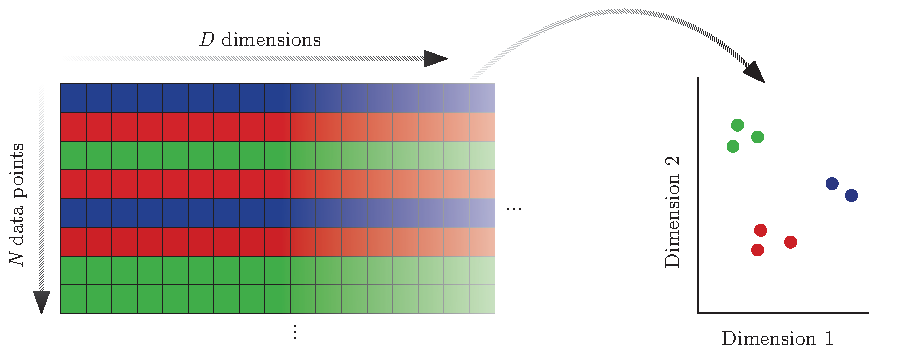
\includegraphics[width=.9\textwidth]{Schema/t-SNE-schema}
	\caption{\gls{t-SNE} schema with toy data. \gls{t-SNE} finds a mapping between the original, high-dimensional data (left) and the data in a lower dimensionality (right). Classes of data points are shown in blue, red and green. Assuming that data points of the same class are more similar to each other, they will be closer to each other in the \gls{t-SNE} visualization.}
	\label{fig:t-SNE-schema}
\end{figure}

% Input activations for DF
\acrlongpl{DF} were trained on the dimensionality-reduced activations belonging to one of the seen classes of the training set. To further improve performance, only activations of correctly predicted training points were used. Some activations of the seen classes might actually strongly differ from the other activations and be wrongly predicted, in which case they should be detected as novelties. The baselines \gls{GMM} and \gls{OC-SVM} both use the same dimensionality-reduced activations as the \acrlongpl{DF} for the hyperparameter search and for fitting the final model with the best found parameters. For all methods based on pre-softmax activations, hyperparameters are found using the scheme of figure \ref{fig:hyperparameter-search}. The same procedure was also applied to error detection, in which case the training set activations of correctly predicted points were used to fit the \gls{GMM}, \gls{OC-SVM} and \acrlong{DF}. These results are only presented in the appendix \ref{app:zurich-figures}.

\subsection{Evaluation}
% CNN
For predictions from trained \gls{CNN} models, accuracy metrics are indicated using precision, recall, \gls{OA} and \gls{AA}(table \ref{table:cm}). For a given set of true class labels, precision measures the percentage of correctly predicted points, while recall measures the number of correctly predicted points over all points predicted as the class.  While \gls{OA} reports the percentage of all data points correctly classified, \gls{AA} calculates the mean of the percentage of correctly classified data points per class. 

\begin{table}[H]
	\centering
	\begin{tabular}{cc|c|c|c|c|cl}
		& & \multicolumn{4}{c|}{True labels y}&\multirow{2}{*}{PA}\\
		\multirow{5}{*}{Predicted labels y} &  & 1& 2& $\hdots$ &r  &\\ \cline{1-7} 
		& 1 &  $n_{11}$ & $n_{12}$ & $\hdots$ & $n_{1r}$& $n_{11}/n_{1\bullet}$ \\ \cline{2-7} 
		& 2 & $n_{21}$ & $n_{22}$ &$\hdots$  &$n_{2r}$ &$n_{22}/n_{2\bullet}$\\ \cline{2-7} 
		& $\vdots$ & $\vdots$ & $\vdots$ &$\ddots$  &$\vdots$&$\vdots$\\ \cline{2-7} 
		& r & $n_{r1}$ & $n_{r2}$ &$\hdots$  & $n_{rr}$ & $n_{rr}/n_{r\bullet}$ \\\cline{1-7} 
		\multicolumn{2}{c|}{UA} & $n_{11}/n_{\bullet 1}$ & $n_{22}/n_{\bullet 2}$ & $\hdots$ & $n_{rr}/n_{\bullet r}$ & OA$=\sum_in_{ii}/n_{\bullet\bullet}$\\
	\end{tabular}
	\caption{\acrlong{CM}: UA = User's Accuracy = Precision, PA = Producer's Accuracy = Recall, OA = Overall Accuracy, $1,2,\hdots,r$=classes. $n_{ij}$ counts the number of labels predicted as class $i$ and belonging to the true class $j$. Bullet indexes signify either the sum of the row (e.g., $n_{O\bullet}$), the sum of the column (e.g., $n_{\bullet O}$) or the sum of all elements of the \acrlong{CM} ($n_{\bullet\bullet}$).}
	\label{table:cm}
\end{table}

% Novelty detection
Evaluation of the confidence measures is made according to the target of novelty detection: We are interested in a binary outcome, predicting whether a new point will belong to one of the seen classes or to an unseen class. All data points belonging to a seen class are attributed a value 0 and all data points belonging to an unseen class a value 1, meaning that they should be detected as different from the other data. In a binary classification setting, true positives are points correctly predicted as positive and true negatives are points correctly predicted as negative. Performance of the uncertainty measures is evaluated using \gls{ROC} curves, which plot the true positives (TP) rate against the true negatives (TN) rate for varying confidence thresholds.  The \gls{AUC} is used to summarize the \gls{ROC} curve (\gls{AUROC}).


\subsection{Hyperparameter Search}
\label{subsec:hyperparameter-search}
% Synthetic dataset
For the synthetic datasets, no hyperparameter search was performed since their only purpose is to show the behaviour of \acrlong{DF} splits visually. Density Trees and \acrlongpl{DF} were trained using the parameters listed in table \ref{table:synthetic-parameters}. The same parameters have been used for each synthetic dataset.

\begin{table}[H]
    \centering
    \small
    \begin{tabular}{ll}
        \toprule
        Parameter & Value \\ \midrule
        \texttt{n\_trees} & 20  \\
        \texttt{subsample\_pct} & .02  \\
        \texttt{max\_depth} & 5 \\
        \texttt{min\_subset} & .02 \\
        \texttt{n\_max\_dim} & -1 \\
        \texttt{ig\_improvement} & .5 \\\bottomrule
    \end{tabular}
    \caption{\acrlong{DF} parameters for each dataset}
    \label{table:synthetic-parameters}
\end{table}

% MNIST, Zurich datasets
For the \gls{MNIST} dataset and the Zurich dataset, best hyperparameters were searched for the novelty detection methods \acrlong{DF}, \gls{OC-SVM} as well as \gls{GMM}. The range of tried parameter combinations are listed in appendix \ref{app:hyperparameters}. For each candidate parameter combination, models were trained in parallel several times on a subset of the training set activations belonging to points of the seen classes being correctly classified and evaluated on a subset of all validation data (fig. \ref{fig:hyperparameter-search})\footnote{For the class ``swimming pools'' of the Zurich dataset, hyperparameters were both trained and evaluated on the training set, since the there are no samples of the ``swimming pools'' class in the validation set.}.

\begin{figure}[H]
    \centering
    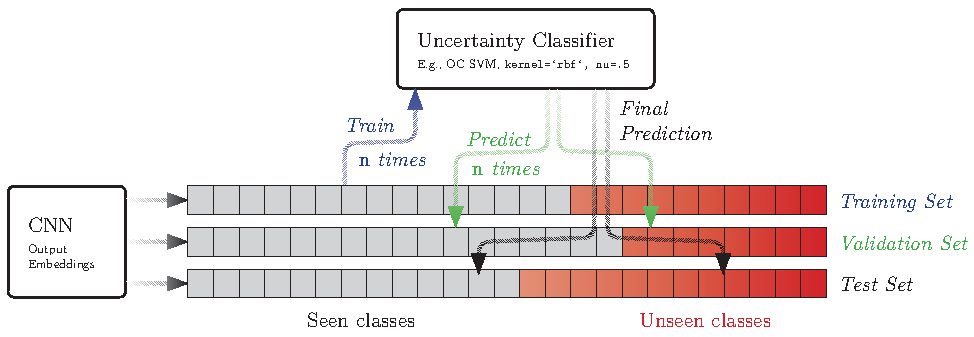
\includegraphics[width=\textwidth]{schema_parameter_search}
    \caption{Parameter Search: Gray boxes show activations belonging to data points of seen classes, red boxes activations belonging to data points of the unseen class. In principle, the true class label is unknown for the test set. For each hyperparameter combination, the classifier is trained \texttt{n} times on a subset of the training set activations belonging only to seen classes (blue arrow) and evaluated on a subset of the seen and unseen points of the validation set (green arrows). The best hyperparameter combination found that way is applied to the entire test set (gray arrows), predicting for every point whether it belongs to a seen or unseen class.}
    \label{fig:hyperparameter-search}
\end{figure}

% Model selection
Finally, the parameter set with the highest \gls{AUROC} is applied to the test set. In addition to finding best hyperparameters, kernel spaces have been visualized for \gls{OC-SVM}  (fig. \ref{fig:oc-svm-vis-rbf} and \ref{fig:oc-svm-vis-poly}). Hyperparameter results and visualizations are shown in appendix \ref{app:hyperparameters}.


\section{Results}

\subsection{Experiments}
% structure
In the following section, the experiments will be presented in the following order: In section \ref{subsec:results-synthetic}, \acrlongpl{DF} will be illustrated by fitting individual Density Trees to the generated synthetic data, visualizing the effects of the Density Tree parameters on the number and shape of generated clusters. In section \ref{subsec:results-MNIST}, \acrlongpl{DF} as well as the baseline confidence measures explained in section \ref{sec:lit} will be applied to the \gls{MNIST} dataset, and their performance will be compared with regards to novelty detection. In section \ref{subsec:results-zurich}, \acrlongpl{DF} as well as the baseline confidence measures will be applied to the Zurich dataset, again measuring performance with respect to novelty detection and highlighting in addition some objects with low confidence values.

\subsection{Synthetic Data}
\label{subsec:results-synthetic}


Figure \ref{fig:gen-data} shows points of the synthetic dataset generated according to the data generator described in section \ref{subsec:data-synthetic} and covariance ellipses of an individual Density Tree trained on all data using the parameters listed in table \ref{table:synthetic-parameters}.

\begin{figure}[H]
    \begin{subfigure}{0.32\textwidth}
        \centering
        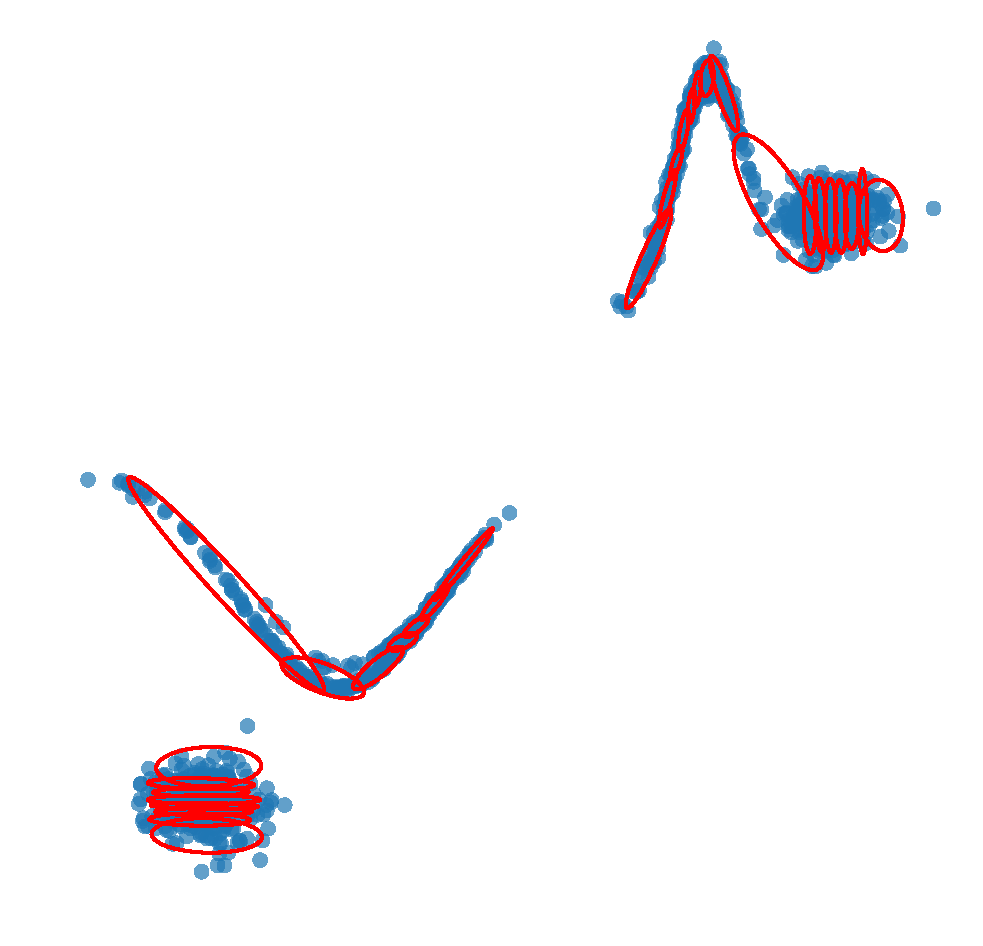
\includegraphics[width=\textwidth]{D1_data-covs}
        \caption{Dataset 1}
    \end{subfigure}
    \begin{subfigure}{0.33\textwidth}
        \centering
        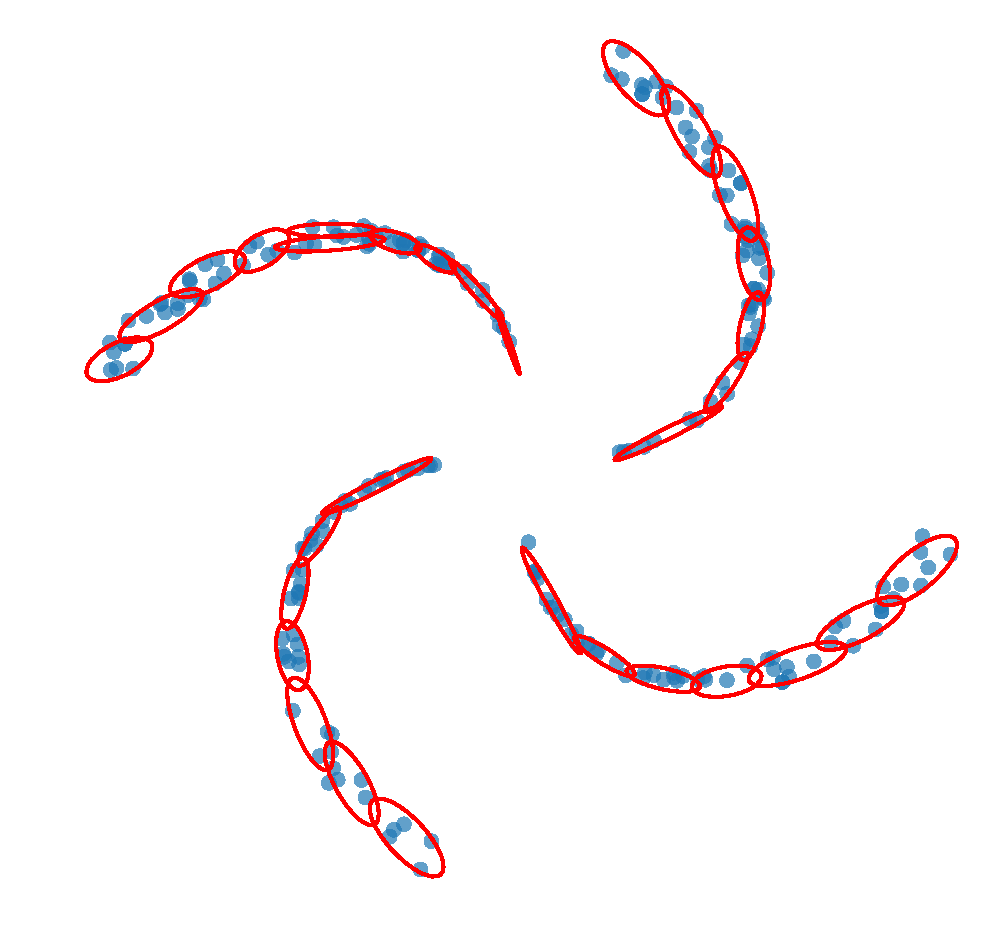
\includegraphics[width=\textwidth]{D2_data-covs}
        \caption{Dataset 2}
    \end{subfigure}
    \begin{subfigure}{0.33\textwidth}
        \centering
        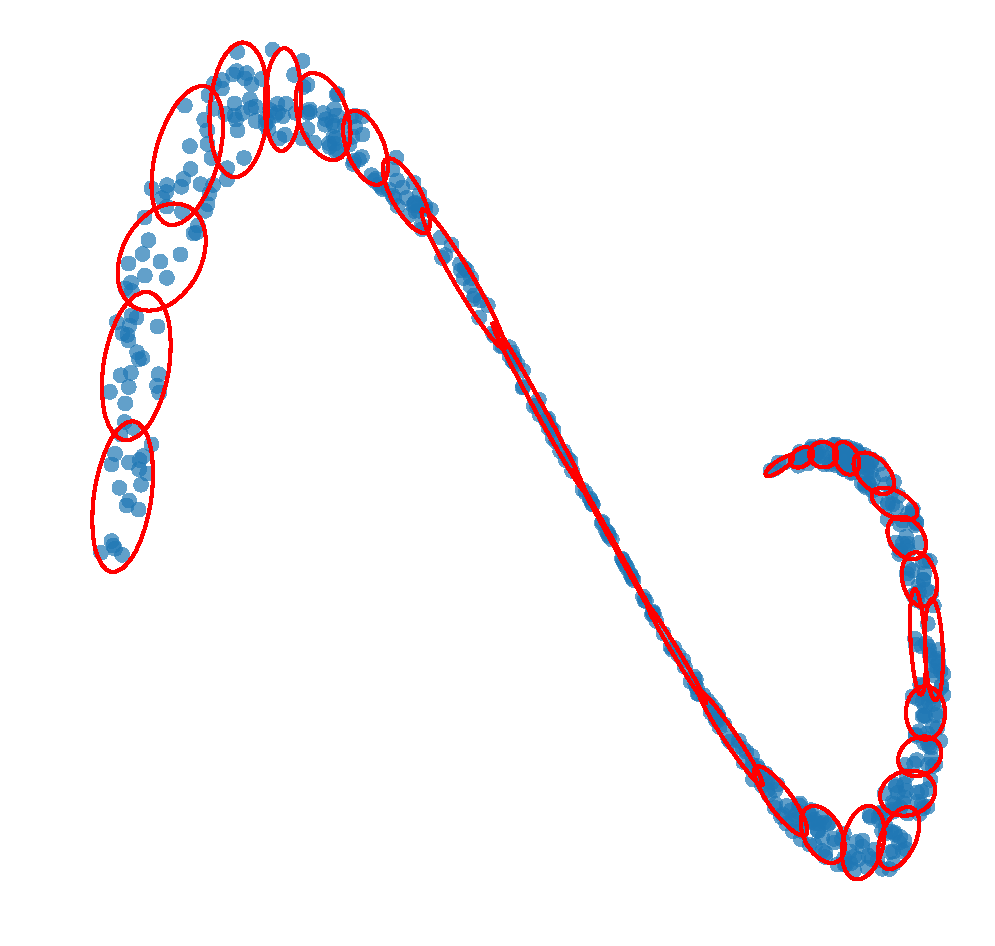
\includegraphics[width=\textwidth]{D3_data-covs}
        \caption{Dataset 3}
    \end{subfigure}
    \caption{Covariance ellipses of individual Density Tree (subset of all points shown)}
    \label{fig:gen-data}
\end{figure}

Figure \ref{fig:D2-covs-steps} shows the covariance ellipses of the splits found at each depth of a Density Tree used to fit dataset 2. With deeper levels of the tree, more splits are created, but only in regions of the spiral arms with fewer points. It seems that in these regions, since there are less points, more ellipses are necessary to fit the local distribution.

% Splitting steps
\begin{figure}[H]
    \centering
    \foreach \depth in {0,...,5}
    {
    \begin{subfigure}{0.32\textwidth}
        \centering
        \includegraphics[width=\textwidth]{D2_data_covs_depth_\depth}
        \caption{Depth = \depth}
    \end{subfigure}
    }
    \caption{Splitting steps of a single node, showing the data, covariance ellipses and information gain of the parent node for dataset 2}
    \label{fig:D2-covs-steps}
\end{figure}

Figure \ref{fig:gen-data-heatmap} shows the Gaussian \gls{PDF} distribution of the corresponding leaf nodes on a regular grid according to one tree and according to a \acrlong{DF} of 20 trees. 

\begin{figure}[H]
    \foreach \name/\dataset/\captionname in {
    one_tree/1/Density Tree,
    one_tree/2/Density Tree,
    one_tree/3/Density Tree,
    DF_forest/1/\acrlong{DF},
    DF_forest/2/\acrlong{DF},
    DF_forest/3/\acrlong{DF}}
    {
    \begin{subfigure}{0.32\textwidth}
        \centering
        \includegraphics[width=\textwidth]{D\dataset_\name}
        \caption{\captionname{} (D\dataset)}
    \end{subfigure}
    }
    \caption{Gaussian \gls{PDF} distribution according to single tree, and according to a \acrlong{DF} consisting of 20 trees}
    \label{fig:gen-data-heatmap}
\end{figure}

While the single tree in figure \ref{fig:gen-data-heatmap} still clearly reflects the ellipsoids visible in figure \ref{fig:gen-data}, the \acrlong{DF} shows a smoother probability distribution. In particularly densely concentrated regions, such as near the central parts of the spiral arms in dataset 2, the density is higher, due to smaller Gaussians being fitted to theses regions.

\subsection{\gls{MNIST}}
\label{subsec:results-MNIST}
% Network accuracies table
Using the \gls{CNN} architecture listed in table \ref{table:CNN_MNIST}, $N=10$ models were trained on all training data except for images belonging to the left-out class. The accuracy of each network was evaluated on training and test points belonging to the seen classes (table \ref{table:mnist-nd-accuracy-mean}). Since classes are balanced in the \gls{MNIST} dataset, only the Overall Accuracy, which is almost identical to Average Accuracy in this case, is indicated. Detailed accuracy measures for each left-out class are shown in appendix \ref{subsec:app-eval-mnist}.

\begin{table}[H]
\centering
    \begin{tabular}{llll}
    \toprule
    Training set & Test set \\\midrule
    99.34 & 99.03  \\\bottomrule
    \end{tabular}
    \caption{Mean Overall Accuracy in \% for the \gls{CNN} models trained on $N-1$ classes}
    \label{table:mnist-nd-accuracy-mean}
\end{table}

% Misclassifications per class
First, predictions were made for the unseen class to inspect the outcome distribution (fig. \ref{fig:pred-count-mnist}). Some left-out classes are mispredicted more homogeneously than others and have a higher mean \gls{MSR}. A possible explanation could be the different visual similarity between certain digits, such as 4 and 9 which may look similar, whereas no digit clearly resembles the digit 8. It is important to notice that higher intrinsic similarity between classes can make the task of novelty detection harder. Prediction counts for all left-out classes are shown in appendix \ref{fig:MNIST_pred_count_all}.

\begin{figure}[H]
    \begin{subfigure}{.49\textwidth}
        \centering
        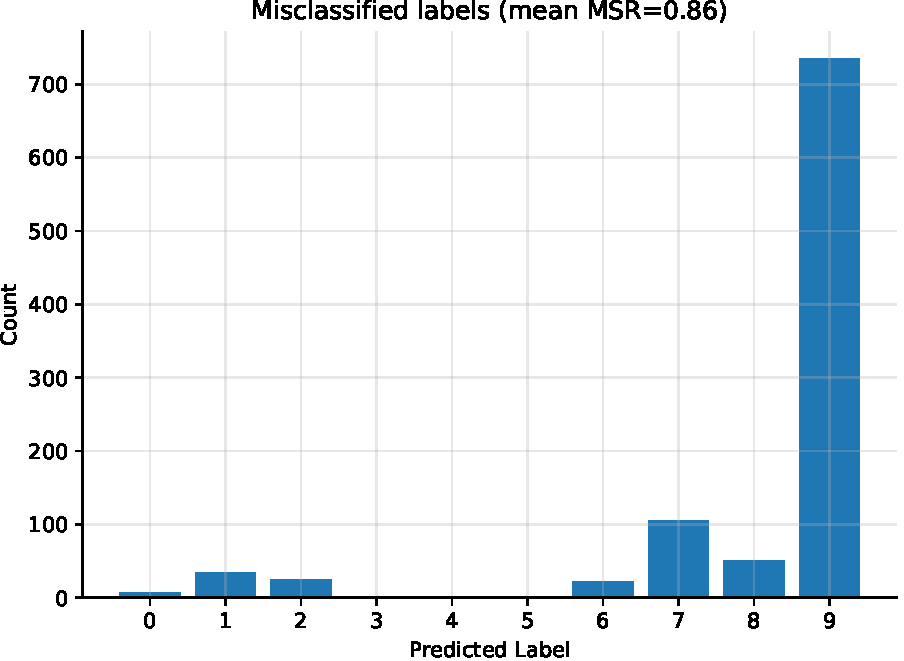
\includegraphics[width=\textwidth]{pred-count_wo_cl4}
        \caption{Left-out class 4}
    \end{subfigure}
    \begin{subfigure}{.5\textwidth}
        \centering
        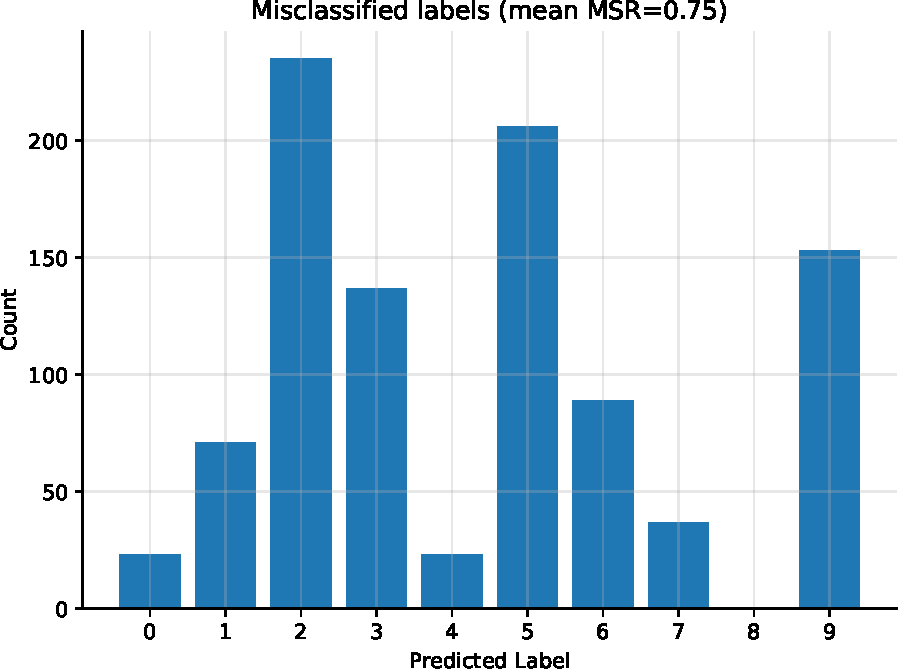
\includegraphics[width=\textwidth]{pred-count_wo_cl8}
        \caption{Left-out class 8}
    \end{subfigure}
   \begin{subfigure}{.49\textwidth}
	\centering
	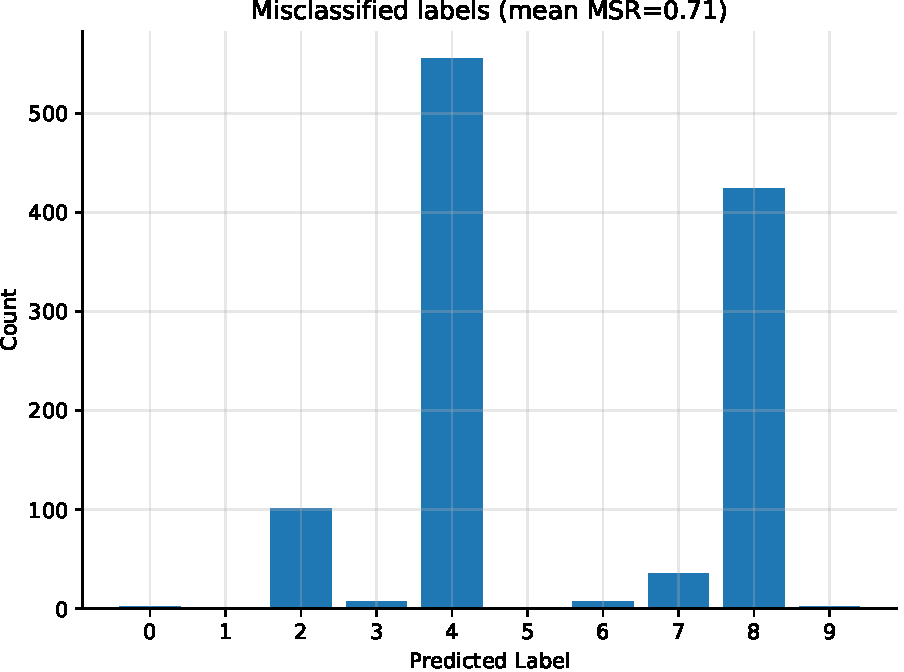
\includegraphics[width=\textwidth]{pred-count_wo_cl1}
	\caption{Left-out class 1}
	\end{subfigure}
	\begin{subfigure}{.5\textwidth}
		\centering
		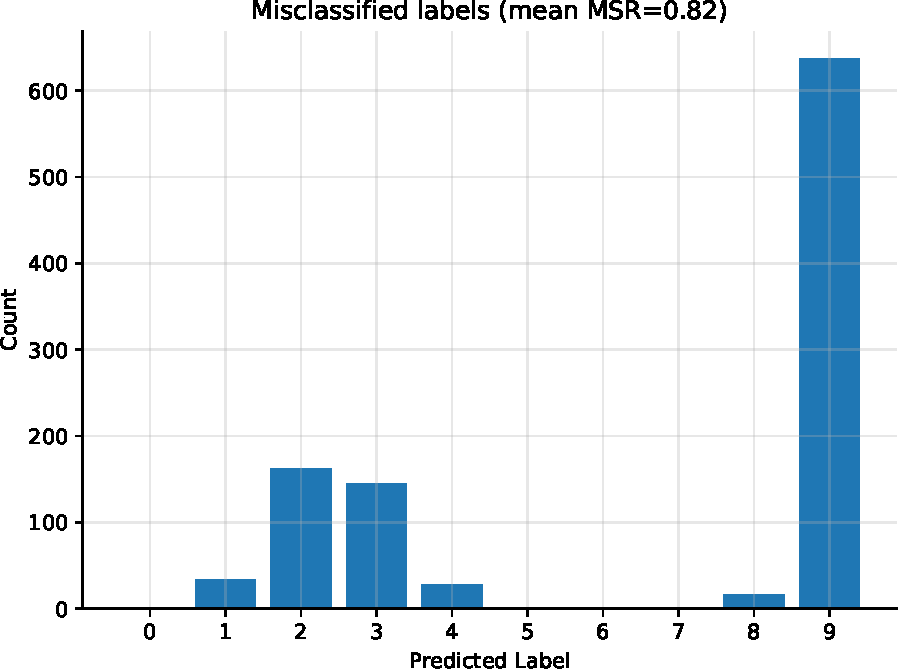
\includegraphics[width=\textwidth]{pred-count_wo_cl7}
		\caption{Left-out class 7}
	\end{subfigure}
    \caption{Predicted labels for networks with left-out classes 4 and 8 (top) and 1 and 7 (bottom). While digits showing a 4 are mostly mislabeled as a 9, the digit 8 is mislabeled less homogeneously. While one could suppose that digits 1 and 7 look similar and might be confused, digits 7 are mostly classified as digit 9, and digit 1 mostly as digits 4 and 8.}
    \label{fig:pred-count-mnist}
\end{figure} 

% Activations, PCA, t-SNE
Second, ReLu activations of the Fully Connected layer were extracted as described in section \ref{subsec:methodology-dim-reduction}. For each image, a vector of 128 activations was retrieved. \gls{PCA} was applied to this vector in order to reduce the redundancy of the filters. For the activations before and after \gls{PCA}, data separability was checked using \gls{t-SNE} visualizations (fig. \ref{fig:tsne-mnist}). The \gls{t-SNE} visualizations in all cases looked similar before and after \gls{PCA}, and are therefore only presented for one of the 10 trained models. \gls{t-SNE} visualizations for activations of each left-out class after \gls{PCA} are shown in appendix \ref{app:mnist-figures}. 

% Class 7 before and after PCA
\begin{figure}[H]
    \centering
    \begin{subfigure}{.49\textwidth}
        \centering
        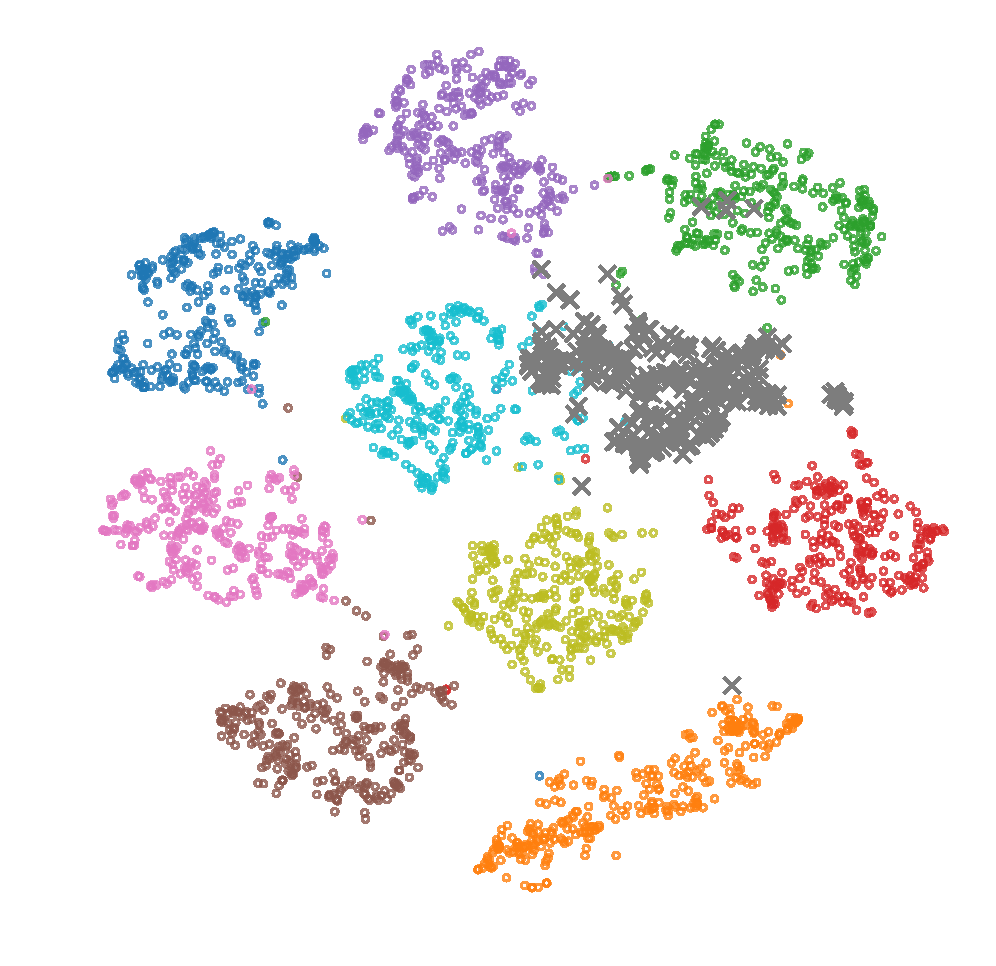
\includegraphics[width=\textwidth]{MNIST_t-SNE_wo_cl_7_before}
        \caption{\gls{t-SNE} before \gls{PCA}}
    \end{subfigure}
    \begin{subfigure}{.5\textwidth}
        \centering
        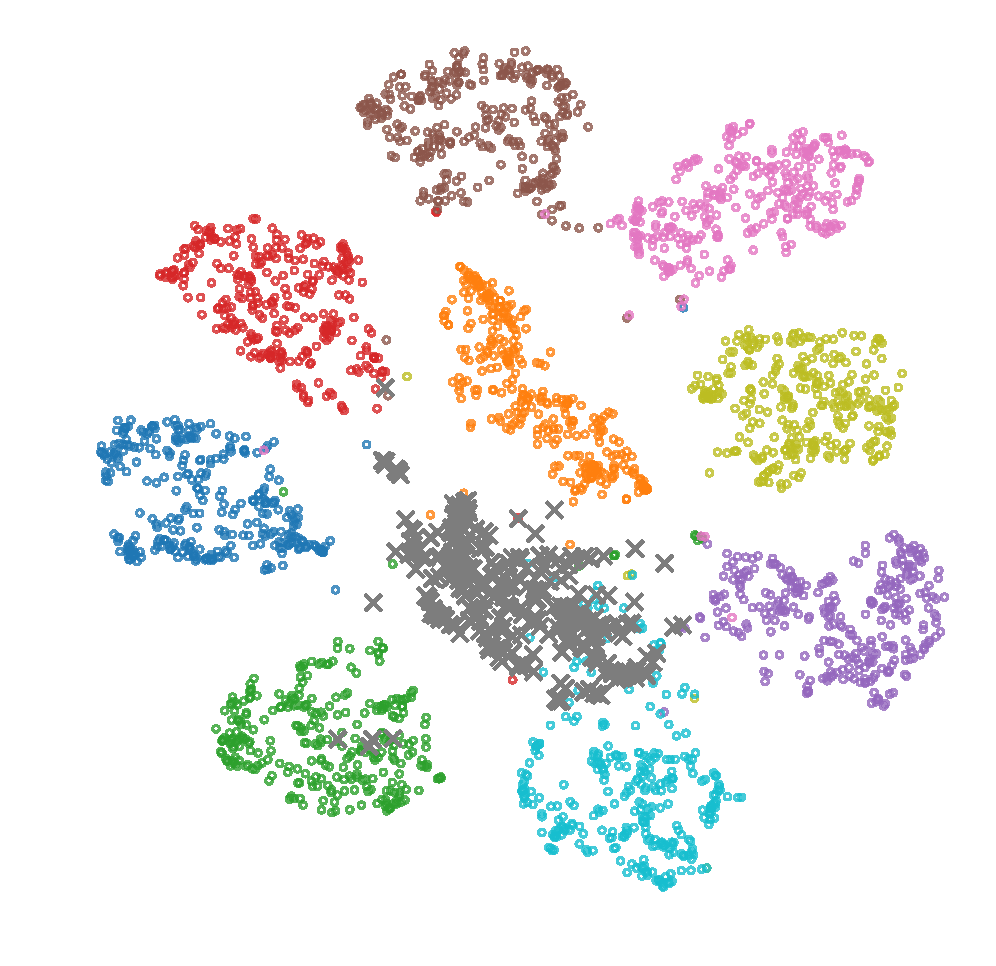
\includegraphics[width=\textwidth]{MNIST_t-SNE_wo_cl_7_after}
        \caption{\gls{t-SNE} after \gls{PCA}}
    \end{subfigure}
    \\[.2cm]
    \legendBulletMNIST
    \caption{\gls{t-SNE} of \gls{MNIST} activations, model with left-out class 7. Both before and after \gls{PCA}, activations of different classes seem well separable, including the unseen class. }
    \label{fig:tsne-mnist}
\end{figure}

Figure \ref{fig:tsne-mnist} shows that the \gls{t-SNE} visualizations of the network activations before and after \gls{PCA} look almost identical. Note that the rotation of the plot before and after applying \gls{PCA} is irrelevant, since the lower-dimensional data representation yielded by \gls{t-SNE} only models the pairwise proximities between data points and not their absolute position in space. 

For novelty detection methods to work well, the unseen class should be well-separated from the other, seen classes. The t-SNE visualization also indicates that all classes are well-separated, including the unseen class. 

The same tendencies with respect to the class confusion shown in figure \ref{fig:pred-count-mnist} can also be observed in the \gls{t-SNE} visualizations (figure \ref{fig:tsne-mnist-miscl}): while class 4 tends to be confused mainly with class 9, class 8 is confused with several clusters.  Unseen class 8 seems to be slightly better separable than unseen class 4, which is very close to class 9.

\begin{figure}[H]
    \centering
    \begin{subfigure}{.49\textwidth}
        \centering
        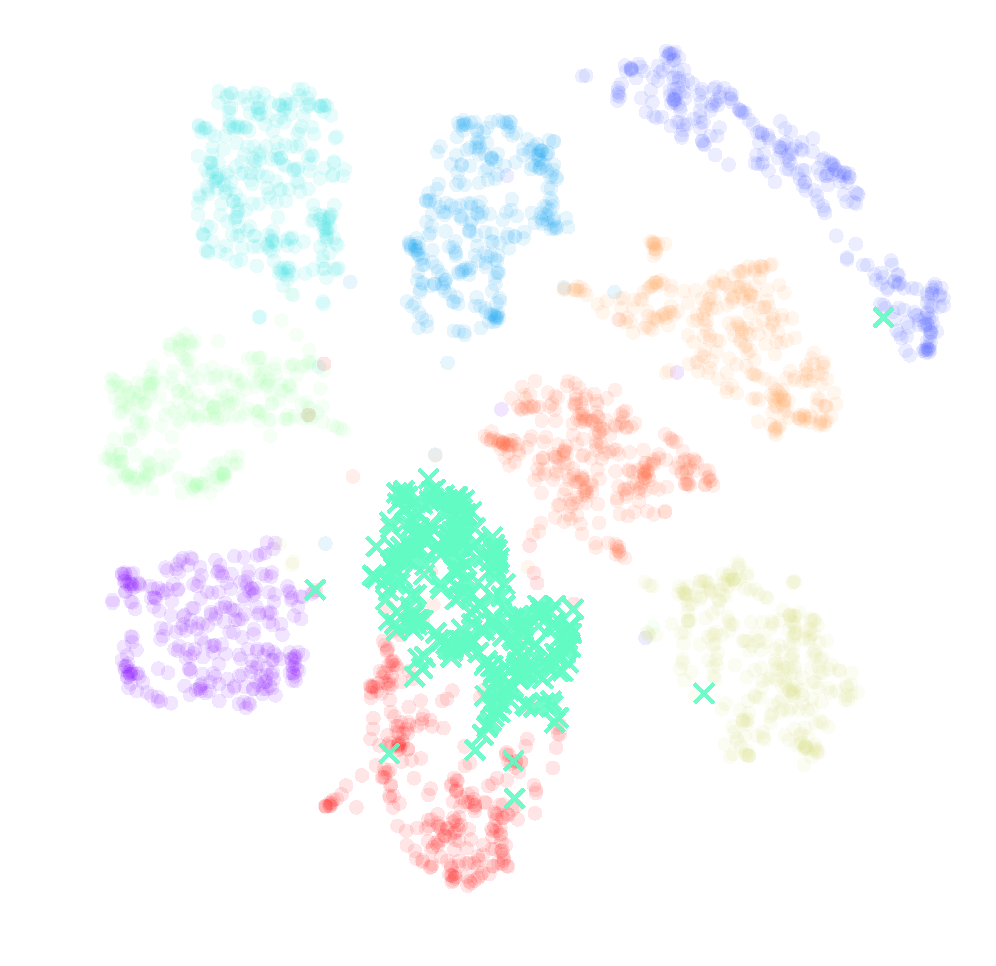
\includegraphics[width=\textwidth]{MNIST_t-SNE_wo_cl_4_after}
        \caption{Class 4}
    \end{subfigure}
    \begin{subfigure}{.5\textwidth}
        \centering
        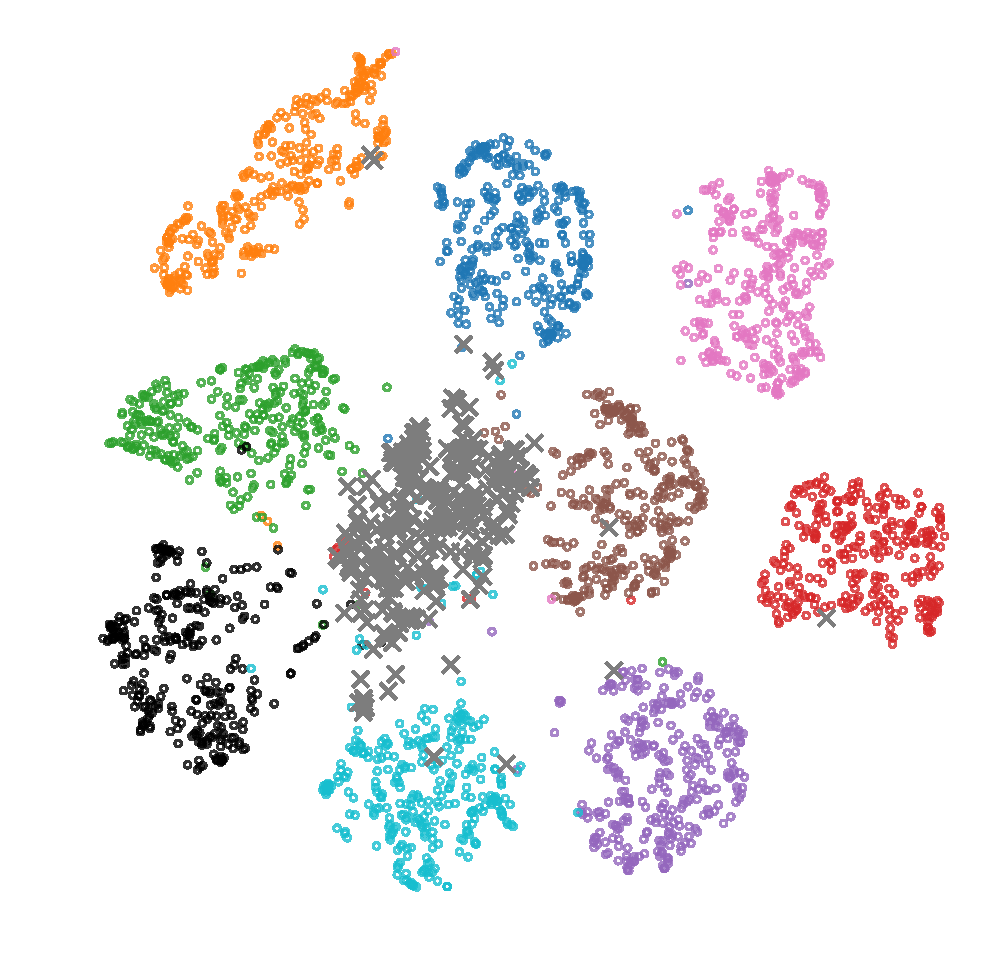
\includegraphics[width=\textwidth]{MNIST_t-SNE_wo_cl_8_after}
        \caption{Class 8}
    \end{subfigure}
    \\[.2cm]
    \legendBulletMNIST
    \caption{t-SNE of \gls{MNIST} activations, after \gls{PCA} transformations.}
    \label{fig:tsne-mnist-miscl}
\end{figure}

% t-SNE and real data
After retrieving the activations of all data points and applying \gls{PCA} dimensionality reduction, parameter search has been performed for \gls{GMM}, \gls{OC-SVM} and \acrlongpl{DF}. Best hyperparameters found for each left-out class and novelty detection method are listed in table \ref{table:hyperparameters-results-mnist}.

\gls{AUROC} metrics for the \acrlong{DF} method and baseline methods are indicated in table \ref{table:mnist-auroc-nd-mean}. Metrics for each class are indicated in appendix table \ref{table:mnist-auroc-nd}.

% ROC table, selected figures
\begin{table}[H]
    \centering
    \begin{tabular}{@{}llllllll@{}}
    \toprule
     \gls{MSR}  & Margin & Entropy & \gls{MC-Dropout} & \gls{GMM} & \gls{OC-SVM}  & \gls{DF} \\ \midrule
    \textbf{0.97} & \textbf{0.97} & \textbf{0.97} & 0.96 & 0.67 & 0.75 & 0.75 \\\bottomrule
    \end{tabular}
    \caption{Mean \gls{AUROC} for each left-out class in the \gls{MNIST} dataset}
    \label{table:mnist-auroc-nd-mean}
\end{table}

In the \gls{MNIST} dataset, \gls{GMM}, \gls{OC-SVM} and \gls{DF} perform worse compared to the baseline methods \gls{MSR}, margin, entropy and \gls{MC-Dropout}. Reasons for the lower performance of the pre-softmax based novelty detection methods are discussed in section \ref{sec:discussion}.


\subsection{Zurich Dataset}
\label{subsec:results-zurich}

% CNN accuracy
\subsection{Overall Results}
Since class imbalance is greater than in the \gls{MNIST} dataset, model performance is indicated for each left-out class separately in table \ref{table:zurich-cnn-acc-nd}. For comparison, accuracy metrics for a \gls{CNN} trained on all classes is given in table \ref{table:zurich-cnn-acc-all}. In this section, illustrations are shown for the model trained on all classes but ``roads'' and the equivalent figures for the other models are shown in appendix \ref{app:zurich-figures}.

% CNN accuracy for full network
\begin{table}[H]
    \centering
    \begin{tabular}{llll}
    \toprule
    Class            & Precision [\%] & Recall [\%] & F1 Score [\%] \\ \midrule
    Roads          &      83.63 &   69.77 &     76.07 \\
    Buildings      &      64.93 &   88.00 &     74.72 \\
    Trees          &      79.80 &   82.69 &     81.22 \\
    Grass          &      94.06 &   67.52 &     78.61 \\
    Bare Soil      &      48.04 &   71.81 &     57.57 \\
    Water          &      97.94 &   91.41 &     94.56 \\
    Railways       &       0.01 &    0.01 &      0.01 \\
    Swimming Pools &      84.75 &   89.80 &     87.20 \\ \midrule
    Average        & 69.15     & 70.13  & 68.75  \\ \bottomrule
    \end{tabular}
    \caption{Test set accuracy for the UNET \gls{CNN} trained on all classes (Overall Accuracy:  77.59 \%)}
    \label{table:zurich-cnn-acc-all}
\end{table}

% CNN accuracy for ND models
\begin{table}[H]
    \centering
    \begin{tabular}{lllllll}
    \toprule
                     & \multicolumn{2}{c}{Training set} & \multicolumn{2}{c}{Validation set} & \multicolumn{2}{c}{Test set}\\
    Left-out Class   & OA [\%]  & AA [\%] & OA [\%]  & AA [\%] & OA [\%]  & AA [\%]\\\midrule
    Roads          &     71.33 &     65.09 &   91.79 &   80.39 &    87.92 &    76.39 \\
    Buildings      &     68.12 &     62.50 &   89.44 &   77.93 &    83.94 &    69.38 \\
    Trees          &     65.36 &     58.84 &   88.79 &   72.59 &    88.58 &    71.40 \\
    Grass          &     57.27 &     54.49 &   79.55 &   68.15 &    81.49 &    69.23 \\
    Bare Soil      &     59.41 &     53.97 &   80.43 &   72.28 &    80.49 &    71.01 \\
    Water          &     65.37 &     62.90 &   85.73 &   71.83 &    84.04 &    68.31 \\
    Railways       &     62.37 &     57.96 &   82.55 &   71.02 &    82.11 &    71.09 \\
    Swimming Pools &     59.56 &     57.72 &   80.55 &   70.50 &    82.34 &    71.34 \\\midrule
    Mean           &  63.60 &  59.18 &  84.85 &  73.09 &  83.86 &  71.02 \\\bottomrule
    \end{tabular}
    \caption{Accuracy measures for the UNET \gls{CNN} trained on $N-1$ classes.}
    \label{table:zurich-cnn-acc-nd}
\end{table}

% Prediction image for ND
A sample visualization of a prediction from a model with the left-out class ``roads'' is shown in figure \ref{fig:pred-gt-road}. Most pixels annotated as ``road'' in the ground truth are either classified as ``buildings'', ``bare soil'' or ``railways''.
\begin{figure}[H]
    \centering
    \begin{subfigure}{0.49\textwidth}
        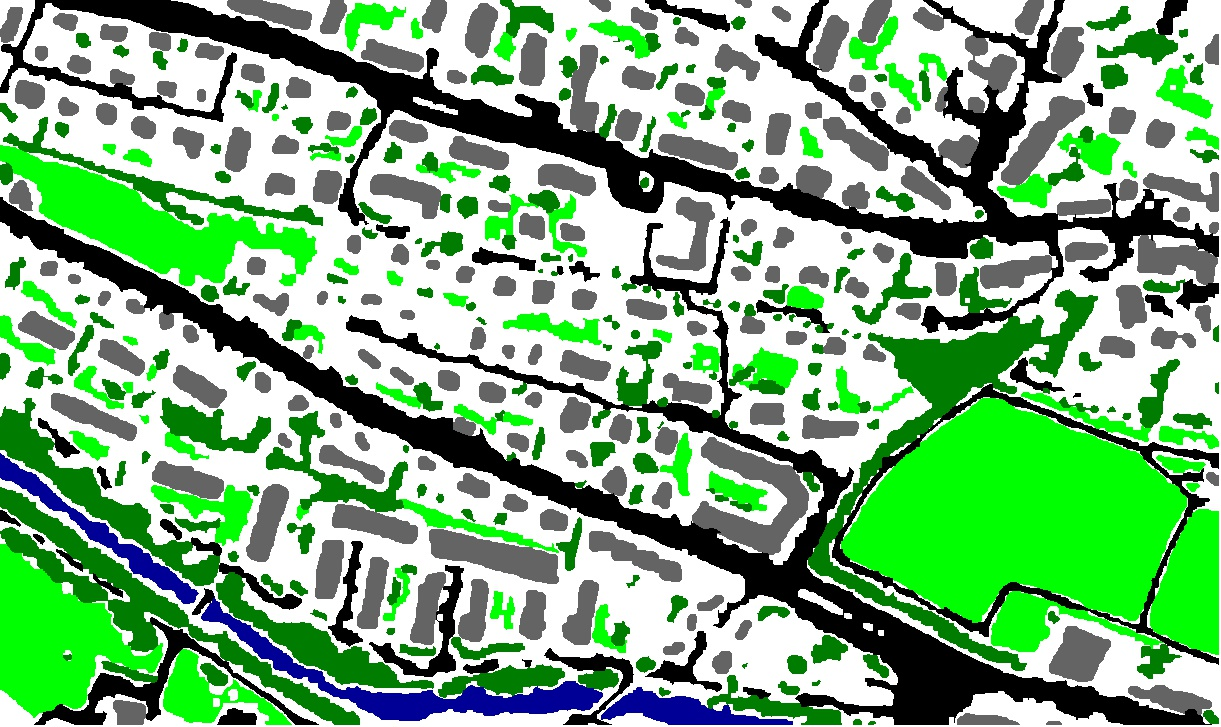
\includegraphics[width=\textwidth]{GT_18}
        \caption{Ground Truth}
    \end{subfigure}
    \begin{subfigure}{0.49\textwidth}
        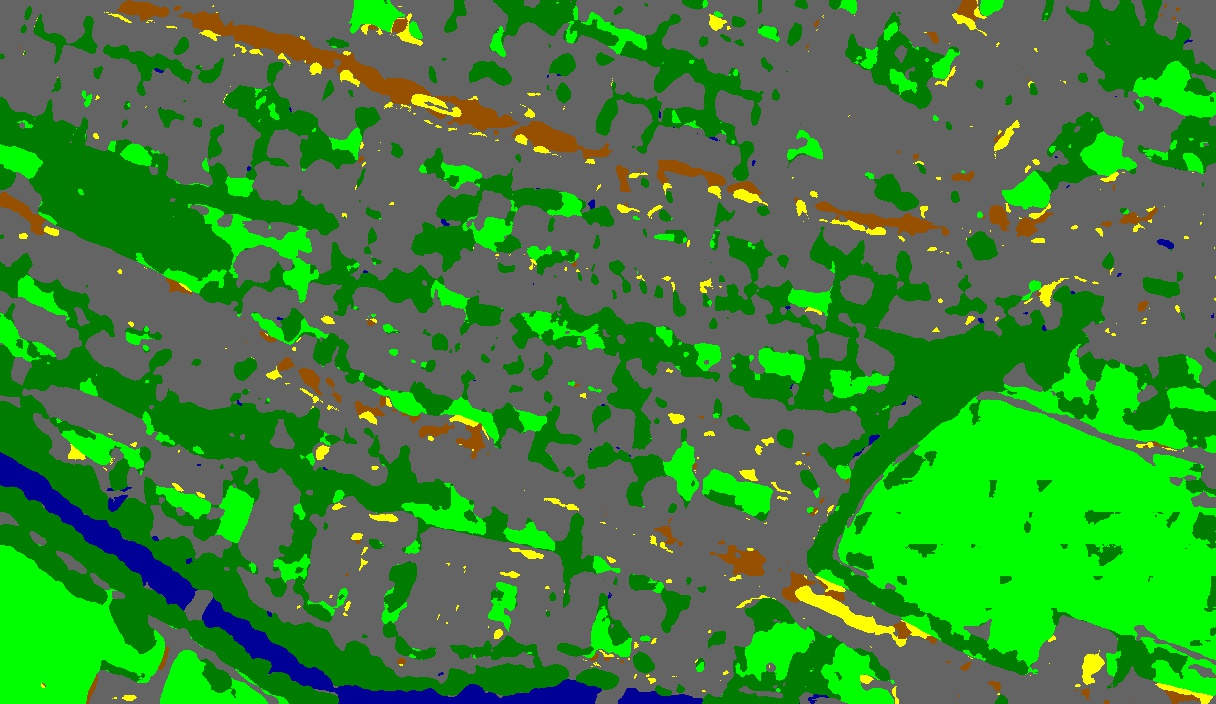
\includegraphics[width=\textwidth]{Im_18_wo_cl_1}
        \caption{Prediction}
    \end{subfigure}
    \\[.2cm]
    \legendH
    \caption{Prediction and ground truth for the model trained without the roads class}
    \label{fig:pred-gt-road}
\end{figure}

% Misclassification distributions
As for the \gls{MNIST} dataset, misclassification distributions were checked for all models (fig. \ref{fig:pred-count-zurich}). Again, more homogeneously misclassified class samples are correlated with higher mean MSR. 

\begin{figure}[H]
    \begin{subfigure}{.49\textwidth}
        \centering
        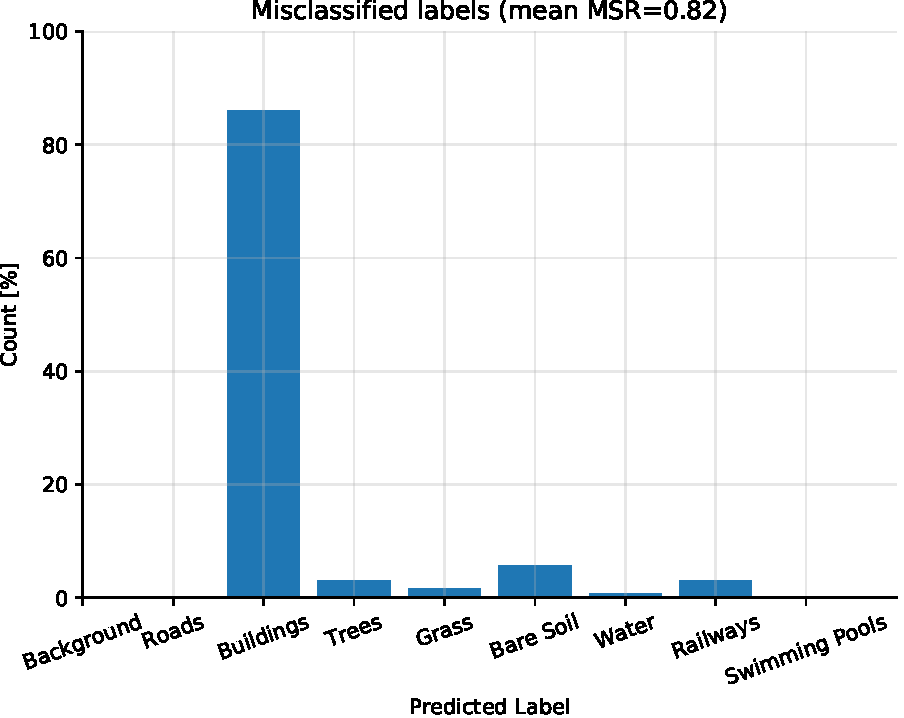
\includegraphics[width=\textwidth]{ZH_pred-count_wo_cl1}
        \caption{Left-out class ``Roads''}
    \end{subfigure}
    \begin{subfigure}{.5\textwidth}
        \centering
        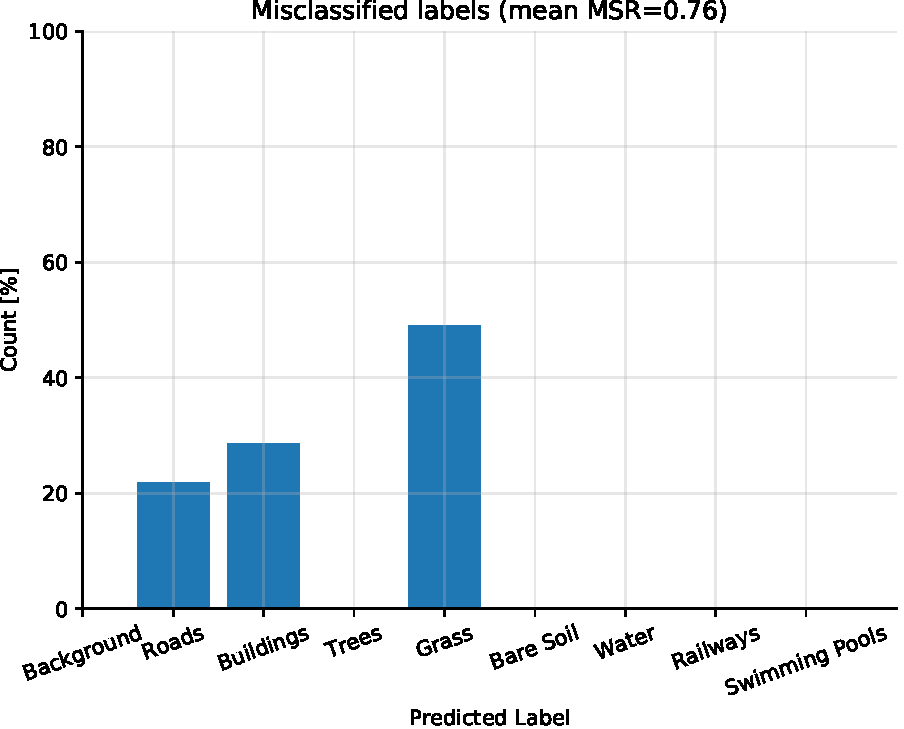
\includegraphics[width=\textwidth]{ZH_pred-count_wo_cl3}
        \caption{Left-out class ``Trees''}
    \end{subfigure}
    \caption{Predictions for network with left-out class ``roads'' and ``trees''. While roads are mostly mislabelled as buildings, trees are mislabelled less homogeneously.}
    \label{fig:pred-count-zurich}
\end{figure} 

% PCA
After training of the network, activations of all images in the training, validation and test sets were retrieved and \gls{PCA} was applied to reduce their dimensionality. The cumulative variance explained by each additional component is shown for the model with the left-out class ``roads'' in figure \ref{fig:pca_components_zurich}. As figure \ref{fig:pca_components} shows, less components are needed to explain a high percentage of the data variance compared to the \gls{MNIST} dataset. 

% t-SNE for separability
Similar to the \gls{MNIST} dataset, it was checked by \gls{t-SNE} visualization if the pre-softmax activations are separable, both before and after \gls{PCA} (fig. \ref{fig:tsne-zurich}). Ideally, both t-SNE plots should show the same relative arrangement between classes. While clusters may be of different sizes, they should be separated according to the classes for a well-enough trained network.

% t-SNE, separable before and after t-SNE
\begin{figure}[H]
    \centering
    \begin{subfigure}{.49\textwidth}
        \centering
        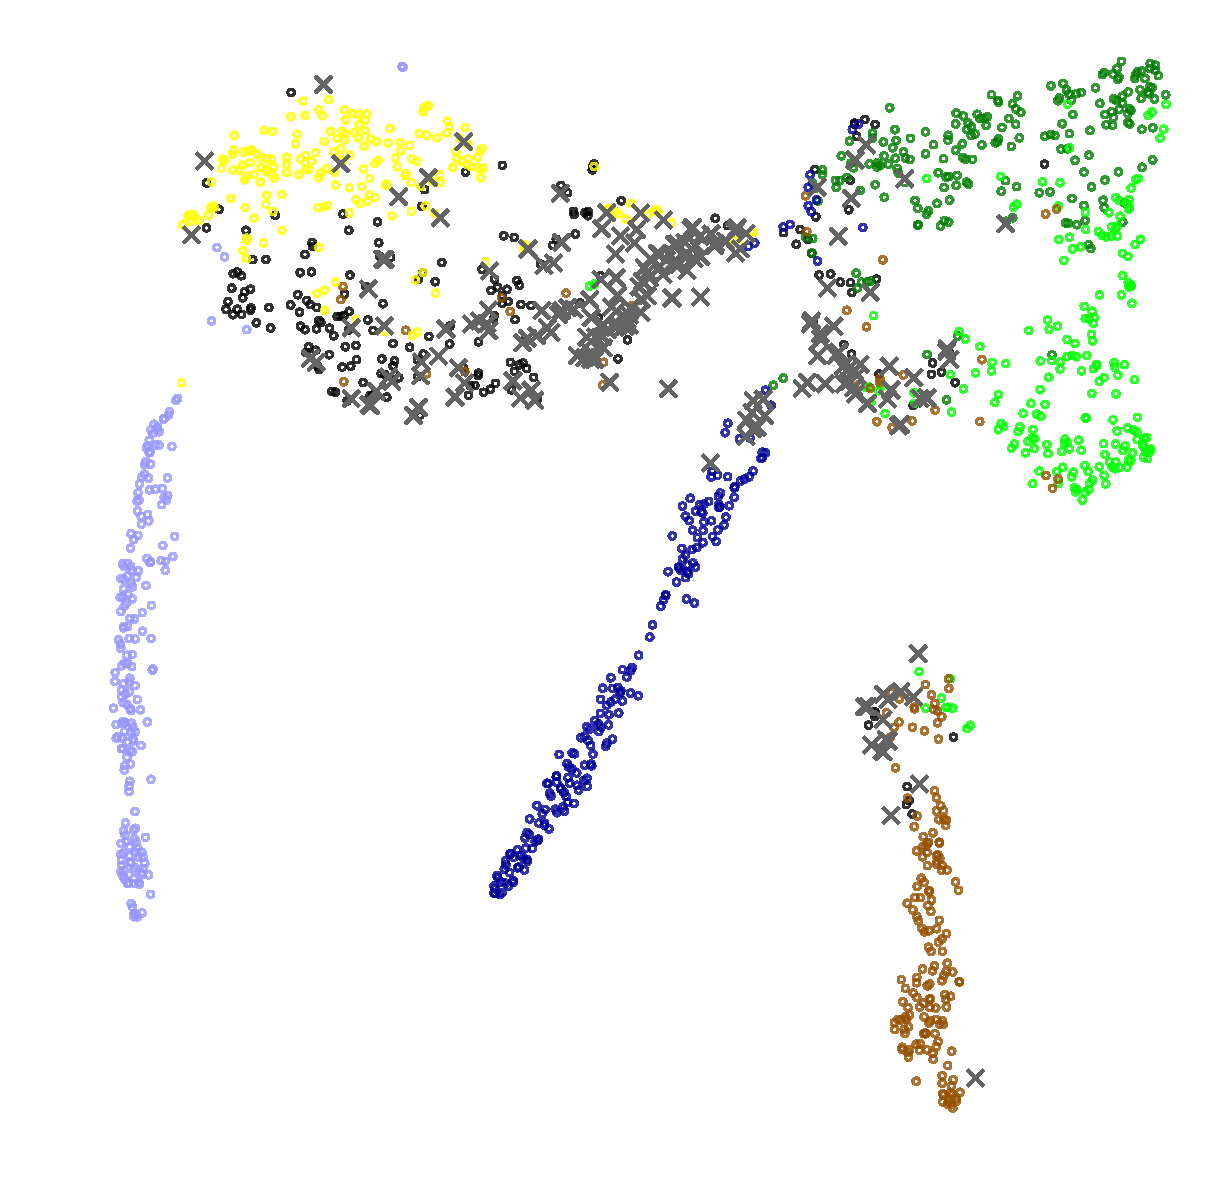
\includegraphics[width=\textwidth]{t-SNE_wo_cl2_before_PCA}
        \caption{\gls{t-SNE} before \gls{PCA}}
    \end{subfigure}
    \begin{subfigure}{.5\textwidth}
        \centering
        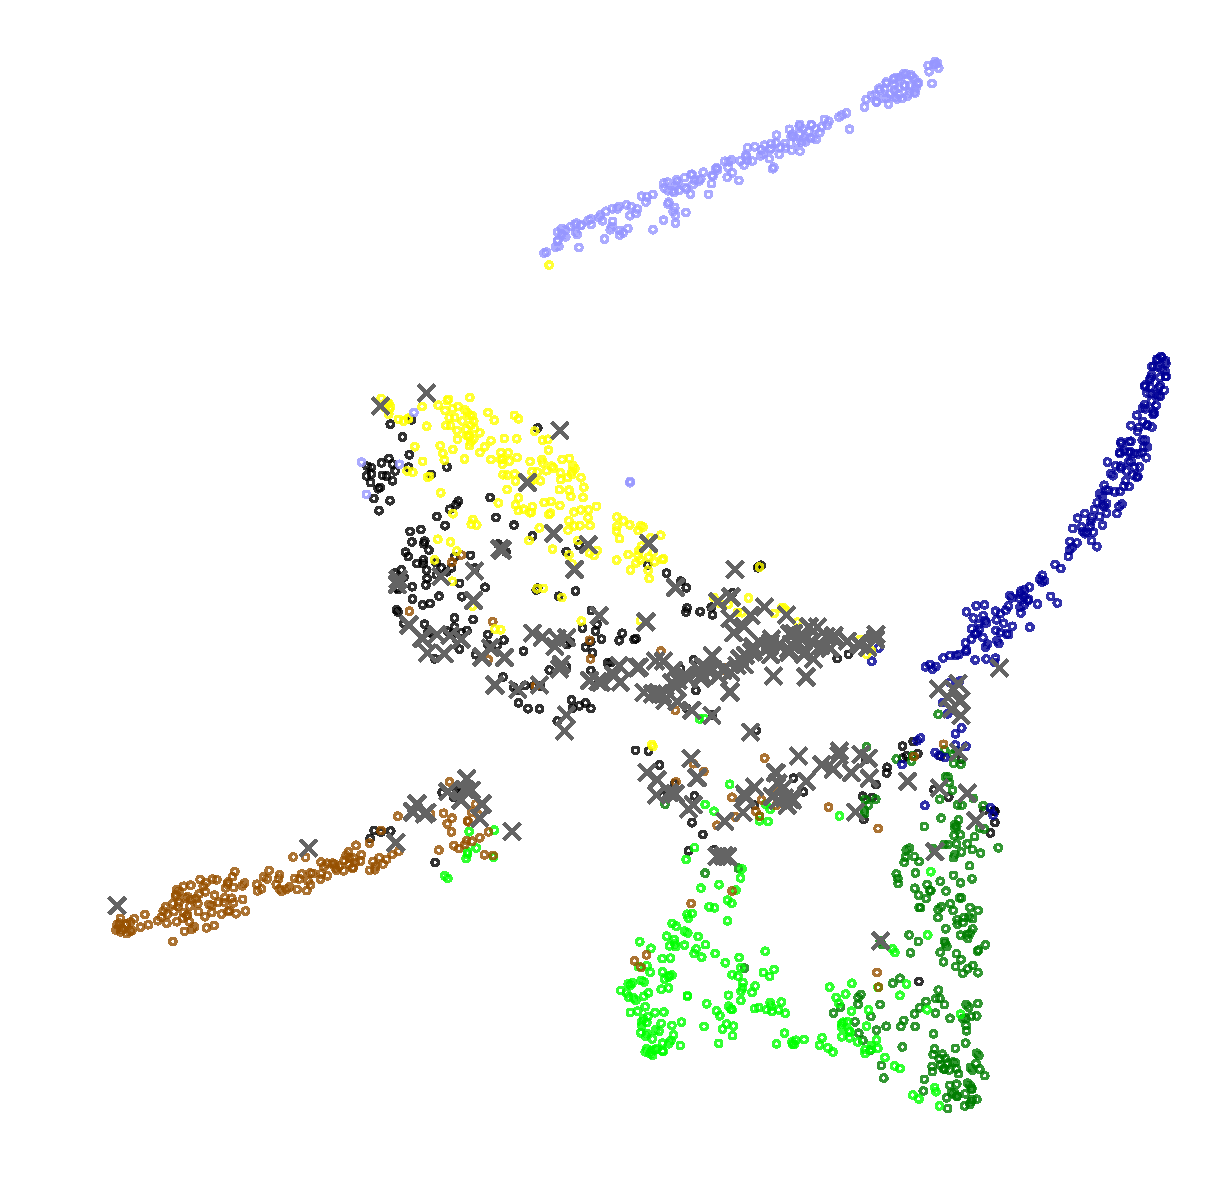
\includegraphics[width=\textwidth]{t-SNE_wo_cl2_after_PCA}
        \caption{\gls{t-SNE} after \gls{PCA}}
    \end{subfigure}
    \\[.2cm]
    \legendBullet
    \caption{\gls{t-SNE} of Zurich dataset activations, model with left-out class buildings. The same number of points are shown by class, although the real class distribution is imbalanced (cf. table \ref{table:zurich-cnn-acc-all}).}
    \label{fig:tsne-zurich}
\end{figure}

Fig \ref{fig:tsne-zurich} shows that \gls{t-SNE} visualizations before and after \gls{PCA} look almost the same. The unseen class ``buildings'' is confused most strongly with the class ``roads'', and partly with the classes ```tree'' and ``grass''. 

\gls{t-SNE} visualizations of the classes ``roads'' and ``trees''  are shown in figure \ref{fig:tsne-zurich-miscl}.

% t-SNE for roads and trees
\begin{figure}[H]
    \centering
    \begin{subfigure}{.49\textwidth}
        \centering
        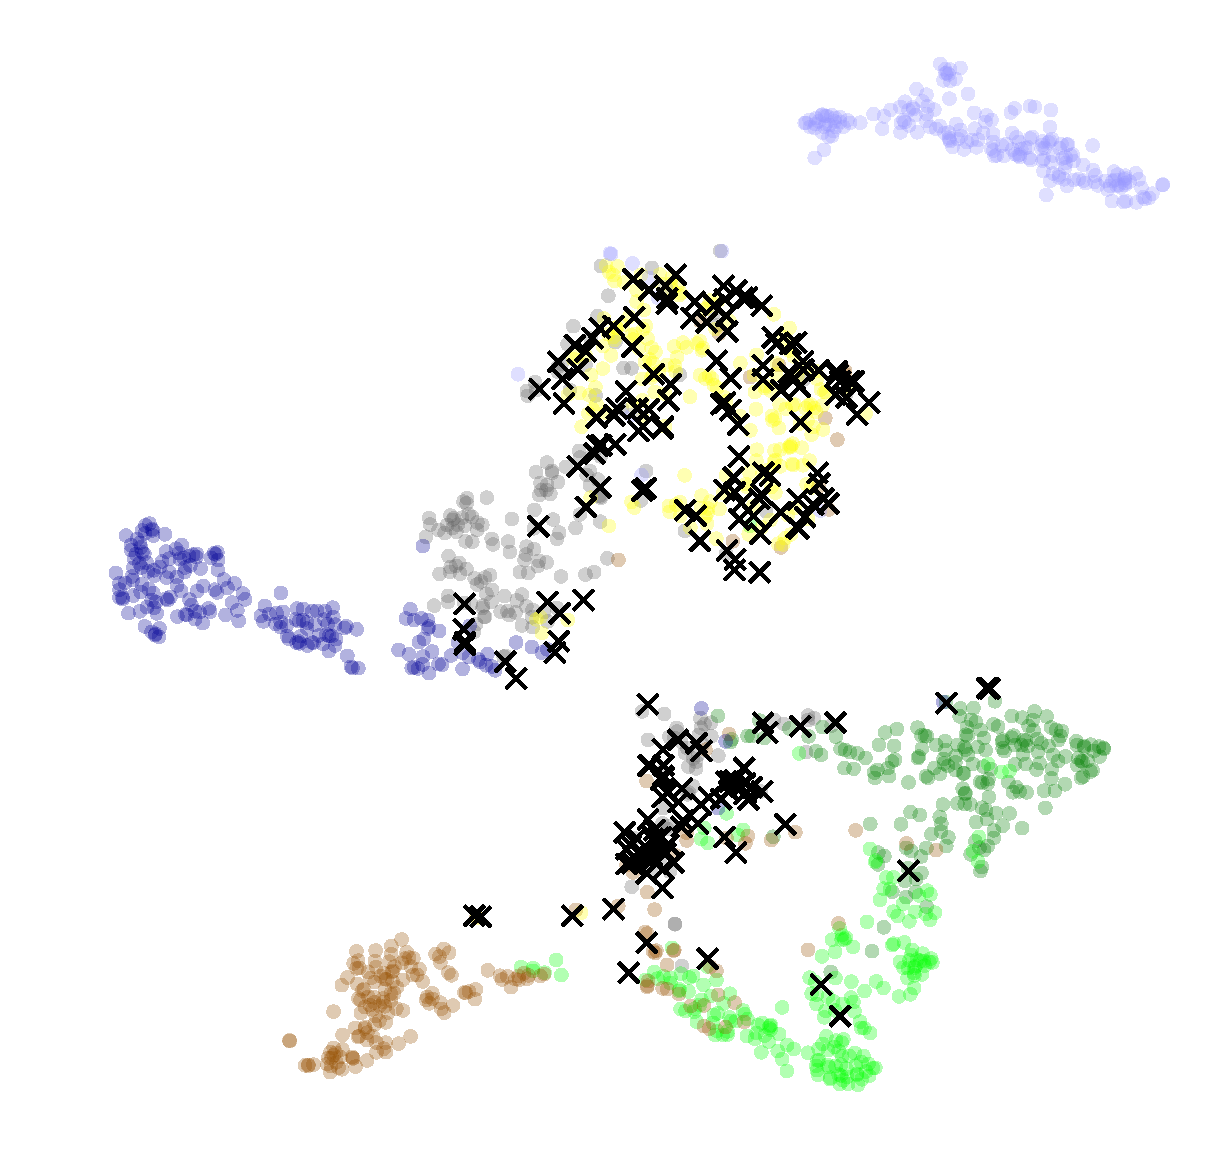
\includegraphics[width=\textwidth]{t-SNE_wo_cl1_after_PCA}
        \caption{Roads}
    \end{subfigure}
    \begin{subfigure}{.5\textwidth}
        \centering
        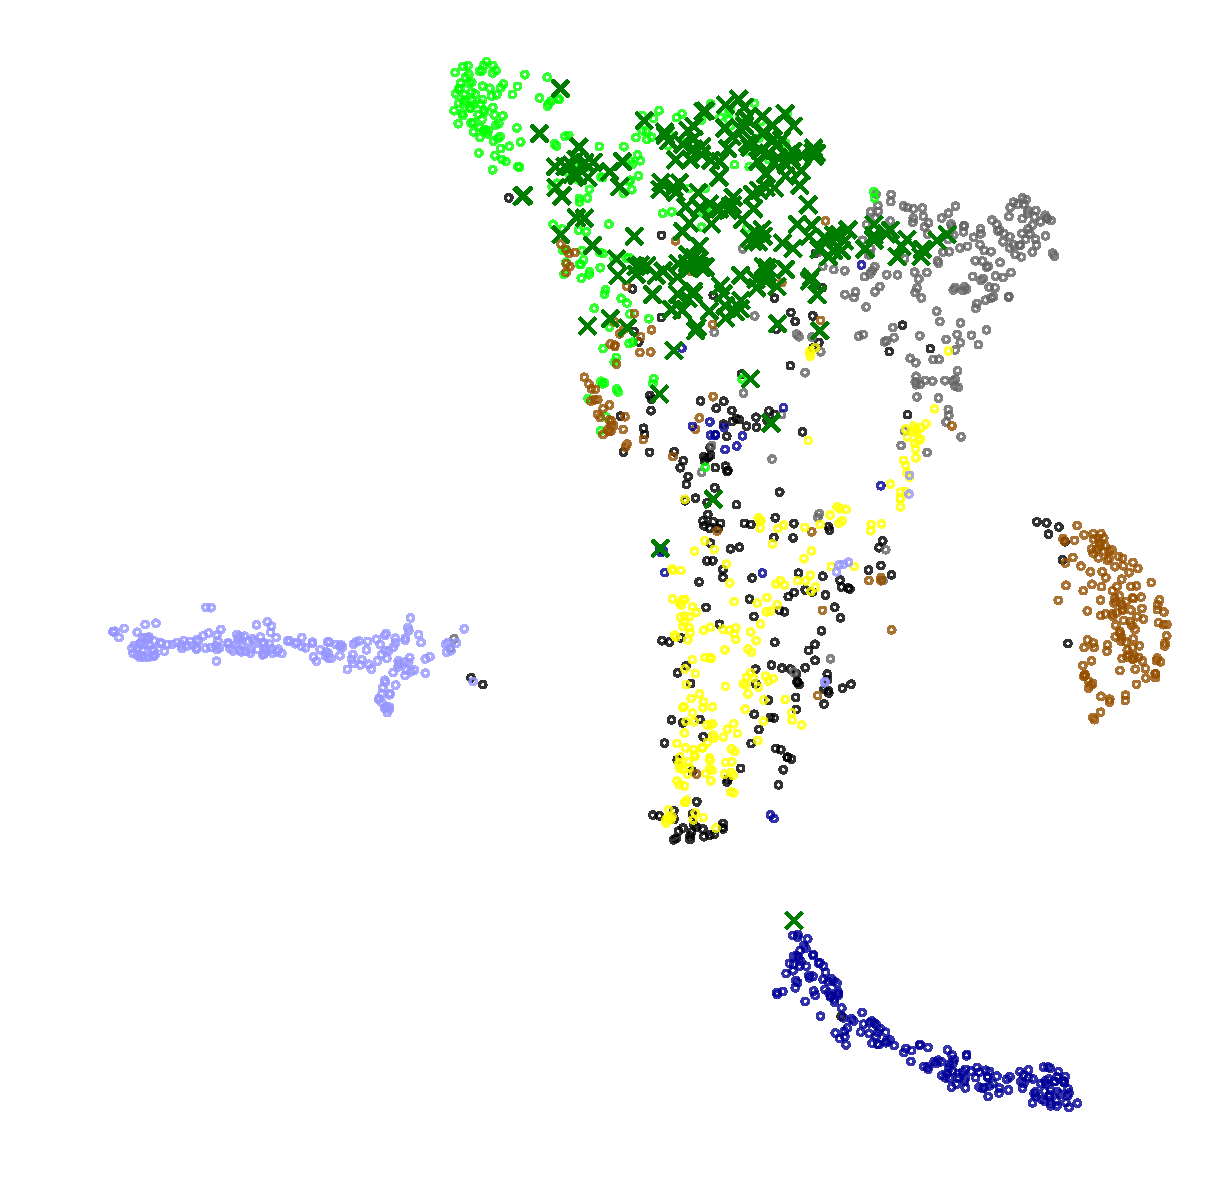
\includegraphics[width=\textwidth]{t-SNE_wo_cl3_after_PCA}
        \caption{Trees}
    \end{subfigure}
    \\[.2cm]
    \legendBullet
    \caption{\gls{t-SNE} of Zurich dataset activations after \gls{PCA}.}
    \label{fig:tsne-zurich-miscl}
\end{figure}
Although there seems to be a confusion between the classes ``roads'' and ``railways'' which suggests difficulties to separate both classes, the class ``railways'' is very rare (fig. \ref{fig:label-dist-zurich}). It is expected that Density Trees first fit ellipses in high-density regions. Therefore, it is likely that a \acrlong{DF} with limited depth will never fits any Gaussians onto the ``railways'' class. Figure \ref{fig:tsne-zurich-all-cl} in appendix shows \gls{t-SNE} of the activations after \gls{PCA} for all left-out classes and for the model trained on all classes. While some classes are always clearly separable from each other, such as bare soil, water and swimming pools, some classes are more mixed together, such as buildings and roads, or grass and trees. It is also noteworthy that some classes are only separable from others when seen during training, such as the class ``water'', while some also remain separable when unseen, such as the class ``swimming pools''.

% Metrics
Best parameters for each left-out class model and novelty detection method are shown in appendix table \ref{table:hyperparameters-results-zurich}. \gls{AUROC} for each left-out class and novelty detection method is shown in table \ref{table:zurich-auroc-nd}.

\begin{table}[H]
    \centering
    \begin{tabular}{@{}lllllllll@{}}
    \toprule
    Left-Out Class & MSR  & Margin     & Entropy & \gls{MC-Dropout} & \gls{GMM}     & \gls{OC-SVM}  & \gls{DF}                \\ \midrule
    Roads          &  0.60 &    0.59 &     0.61 &     0.59 &  0.66 &    0.50 &  \textbf{0.70} \\
    Buildings      &  0.65 &    \textbf{0.66} &     0.65 &     0.65 &  0.58 &    0.63 &  0.64 \\
    Trees          &  0.74 &    0.74 &     0.74 &     0.75 &  0.66 &    \textbf{0.76} &  0.56 \\
    Grass          &  0.38 &    0.37 &     0.39 &     0.39 &  0.47 &    0.31 &  \textbf{0.54} \\
    Bare Soil      &  0.68 &    0.70 &     0.63 &     0.60 &  0.66 &    \textbf{0.78} &  0.65 \\
    Water          &  0.59 &    0.60 &     0.58 &     0.58 &  0.59 &    0.39 &  \textbf{0.64} \\
    Railways       &  0.57 &    \textbf{0.59} &     0.53 &     0.54 &  0.44 &    0.52 &  0.37 \\
    Swimming Pools &  0.26 &    0.28 &     0.23 &     0.28 &  \textbf{0.99} &    0.97 &  \textbf{0.99} \\\midrule
    Average        &  0.56 & 0.57 & 0.55 & 0.55 & 0.63 & 0.61 & \textbf{0.64} \\\bottomrule
    \end{tabular}
    \caption{\gls{AUROC} for each left-out class}
    \label{table:zurich-auroc-nd}
\end{table}

% AUROC numbers
Table \ref{table:zurich-auroc-nd} indicate that the \gls{DF} outperforms other novelty detection methods in 3 of 8 classes and pre-softmax-based methods \gls{GMM}, \gls{OC-SVM} and \gls{DF} together outperform the softmax-based methods in 6 out of 8 classes. \gls{DF} clearly outperforms other methods on the Roads and Water classes. Pre-softmax based methods clearly outperform softmax-based methods on the Swimming Pools class. Visual results of the different methods are shown in appendix figures \ref{fig:zurich-im-uncert-1} - \ref{fig:zurich-im-uncert-2}. \gls{ROC} curves used to produce the \gls{AUROC} metrics of table \ref{table:zurich-auroc-nd} are shown in appendix figure \ref{fig:zurich-nd-roc}.

\subsection{Visual interpretation}

% Visual results
To illustrate the performance of the novelty detection methods, confidence images for individual left-out classes can be analyzed and visualized. In this section, results are compared according to the classes on which the \acrlong{DF} performs better or worse than baseline methods. Visual examples are provided for MSR and \acrlongpl{DF}. Figures for all methods and left-out classes are shown in appendix figures \ref{fig:zurich-im-uncert-1} - \ref{fig:zurich-im-uncert-8}.

% Histogram equalization, distribution
A property of novelty detection methods is that they attribute extreme values to outliers, leading to skewed distributions of the confidence values. This can be observed in the results of the methods \gls{GMM}, \gls{OC-SVM} and \gls{DF}. In the case of novelty detection, some particular objects of the image may be recognized as very uncertain, leading to lesser visibility of confidence differences in the rest of the image. Therefore, histogram equalization was applied to the confidence images of \gls{GMM}, \gls{OC-SVM} and \gls{DF} to enhance the overall image contrast and show more local differences between classes \cite{Gonzlez2012DigitalIP}. Individual objects with very high uncertainty are shown using the original image (fig.  \ref{fig:hist-eq}).

% Histogram equalization
\begin{figure}[H]
    \centering
    \begin{subfigure}{.49\textwidth}
        \centering
        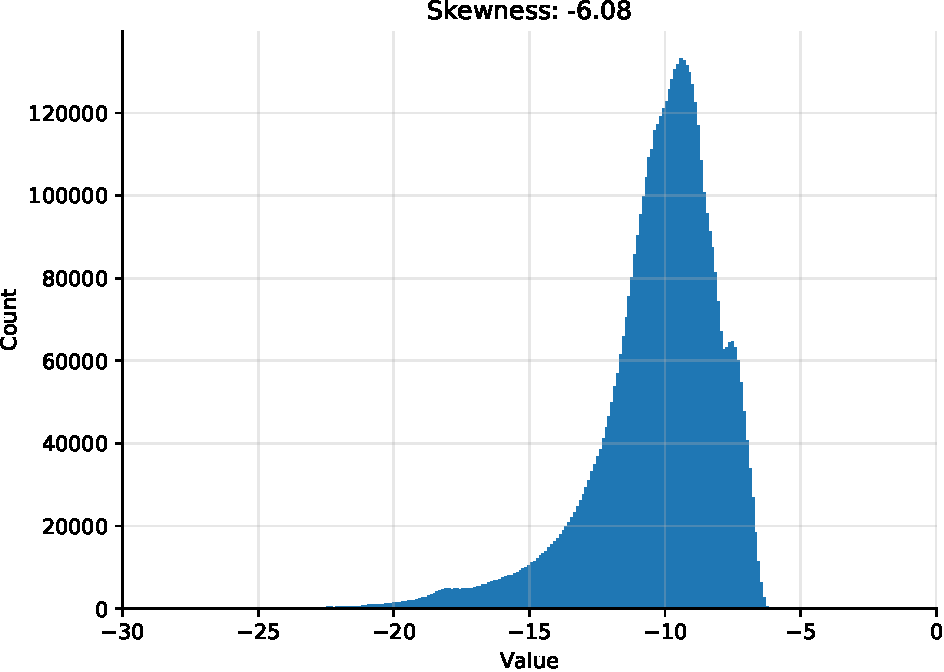
\includegraphics[width=\textwidth]{Skew_GMM_wo_cl1}
        \caption{Original histogram}
    \end{subfigure}
    \begin{subfigure}{.49\textwidth}
        \centering
        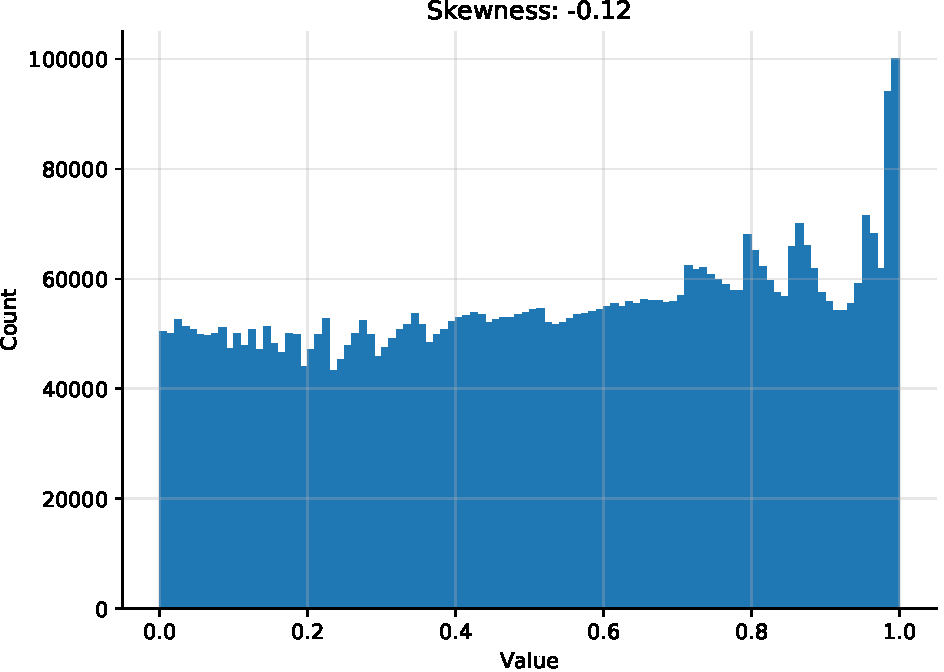
\includegraphics[width=\textwidth]{Skew_GMM_wo_cl1_eq}
        \caption{Equalized histogram}
    \end{subfigure}
    \begin{subfigure}{.45\textwidth}
        \centering
        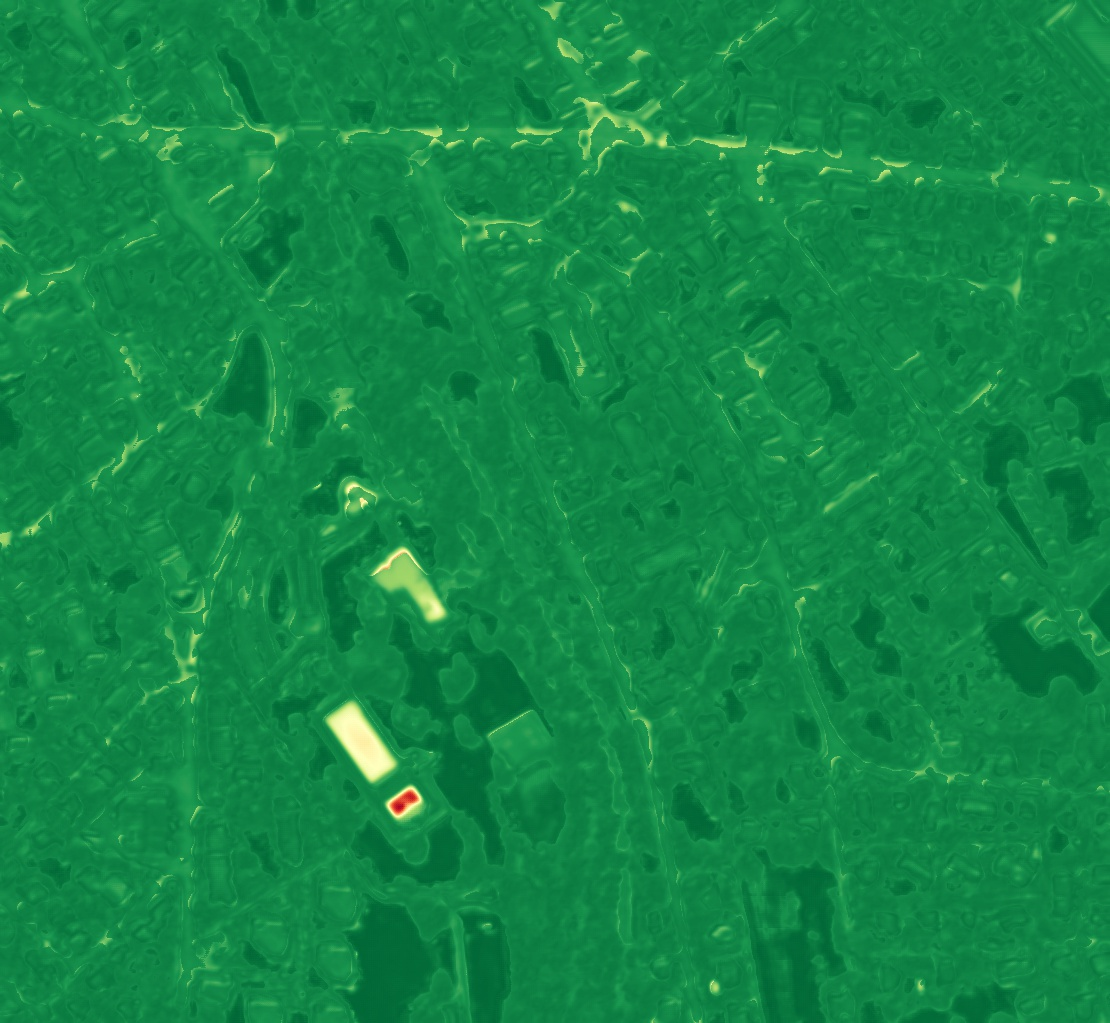
\includegraphics[width=\textwidth]{Figures/ZH_wo_cl_1_df_im_1}
        \caption{Original confidence image}
        \label{subfig:original-im}
    \end{subfigure}
    \begin{subfigure}{.45\textwidth}
        \centering
        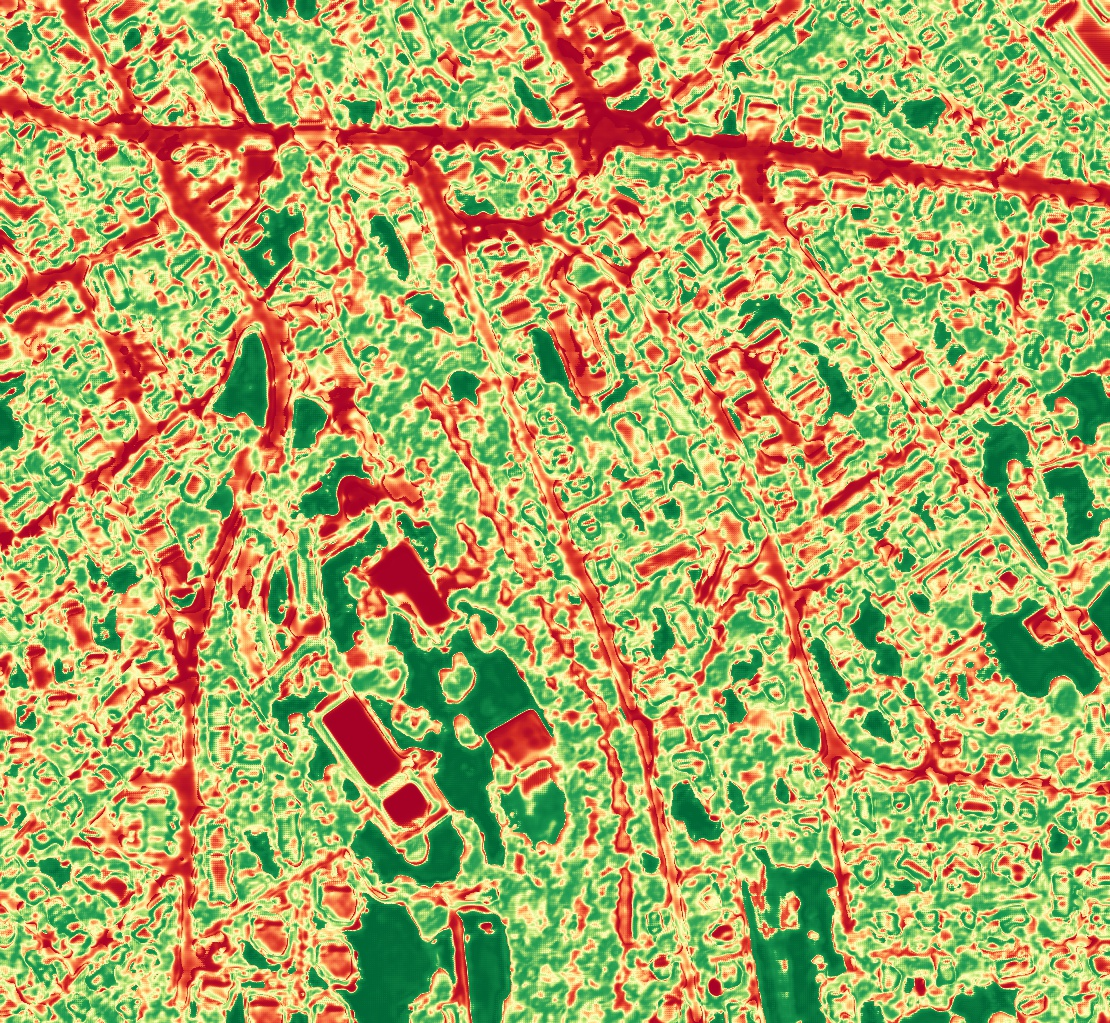
\includegraphics[width=\textwidth]{ZH_wo_cl_1_df_im_1_eq}
        \caption{Equalized confidence image}
        \label{subfig:equalized-im}
    \end{subfigure}
    \textsc{Certainty}\\[.2cm]
    \legendCert
    \caption{Original and equalized confidence distributions for \gls{DF}, using the left-out class ``Roads''. While outliers are visible in the original figure, smaller confidence differences between classes are better visible after histogram equalization.}
    \label{fig:hist-eq}
\end{figure}

Figure \ref{fig:im_cert_1} shows visual results for the class ``roads''. \acrlong{DF} here outperforms the other methods, confirming visually that it has the highest \gls{AUROC} values of all confidence estimation methods (table \ref{table:zurich-auroc-nd}). The unseen class ``Roads'' clearly appears to be the least certain, while for MSR, the roads seem as uncertain as other classes. MSR just like margin and entropy, the other baseline methods based on the softmax output, mainly show low certainty along class changes (figure \ref{fig:zurich-im-uncert-1}.

% Acc MSR, OC-SVM, DF
\newcommand{\imcert}[3]{ % arguments: classname, classremoved, im
\begin{figure}[H]
    \centering
    \begin{subfigure}{0.48\textwidth}
        \includegraphics[width=\textwidth]{ZH_wo_cl_#2_net_msr_im_#3}
        \caption{MSR}
    \end{subfigure}
    \begin{subfigure}{0.48\textwidth}
        \includegraphics[width=\textwidth]{ZH_wo_cl_#2_svm_im_#3_eq}
        \caption{\gls{OC-SVM}}
    \end{subfigure}
    \begin{subfigure}{0.48\textwidth}
        \includegraphics[width=\textwidth]{ZH_wo_cl_#2_df_im_#3_eq}
        \caption{\gls{DF}}
    \end{subfigure}
    \begin{subfigure}{0.48\textwidth}
        \includegraphics[width=\textwidth]{GT_18}
        \caption{Ground Truth}
    \end{subfigure}
    \begin{subfigure}{0.48\textwidth}
        \includegraphics[width=\textwidth]{ZH_pca_components_wo_cl_#2}
        \caption{\gls{PCA} components}
    \end{subfigure}
    \begin{subfigure}{0.38\textwidth}
        \includegraphics[width=\textwidth]{ROC_pred_wo_cl_#2}
        \caption{ROC}
    \end{subfigure}
    \\[.2cm]    
    \legendGTandCert
    \caption{Visual uncertainty results for selected methods on left-out class ``#1'' and corresponding ground truth. Contrast stretching and histogram equalization have been applied to \gls{OC-SVM} and \gls{DF} images for better visibility. Variance per \gls{PCA} component and \gls{ROC} curves are shown below the confidence images.}
    \label{fig:im_cert_#2}
\end{figure}
}
\imcert{Roads}{1}{3}

% Comparison roads, trees
Figure \ref{fig:im_cert_3} shows a class for which the \acrlong{DF} underperforms. In this case, OC-SVM shows the best performance in detecting the unseen class ``trees'' (along the river and on the top-right side of the field). While both the winning method OC-SVM and DF show low confidence in the regions containing trees, the \acrlong{DF} in addition shows very low confidence along the river and along some parts of the roads.

\imcert{Trees}{3}{3}

% PCA, ROC
For both left-out classes roads and trees, a low number of \gls{PCA} components are needed to explain the initial variance of activations. Visual results, explained variance by \gls{PCA} components and \gls{ROC} curves are provided for all left-out classes in appendix \ref{app:zurich-figures}.

% t-SNE for all classes
Figure \ref{fig:t-SNE-probas_3} shows the confidence values of the different methods for the left-out class ``trees'' on a subset of all points used to produce the \gls{t-SNE} visualizations. All points with a solid border belong to the unseen class. Ideally, those points should be colored red (uncertain) while points of other classes should be yellow or green. Figure \ref{fig:t-SNE-probas_3} also shows different behavior in the seen classes between novelty detection methods. Softmax-based methods \gls{MSR}, margin, entropy and \gls{MC-Dropout} all behave similarly and identify the regions of lowest confidence at the borders of clusters and within the unseen class. The pre-softmax based confidence measures \gls{GMM}, \gls{OC-SVM} and \gls{DF} behave similarly and generally attribute a higher confidence to the cluster centers and unseen class, while \gls{GMM} and \gls{DF} also attribute lower certainty to points of the class ``bare soil' and identify the class ``swimming pool'' as particularly uncertain, which could indicate their ability better identify heterogeneous classes, such as ``bare soil'', and classes with few samples, such as ``swimming pools''.

% t-SNE for all classes
\newgeometry{left=1cm,right=1cm,top=2cm,bottom=2cm}
\newcommand{\imCertTsne}[2]{ % arguments: classname, classremoved, im
\begin{figure}[H]
    \centering
    \begin{subfigure}{.3\textwidth}
            \centering
            \includegraphics[width=\textwidth]{t-SNE_wo_cl#1_after_PCA}
            \caption{\gls{t-SNE}}
    \end{subfigure}
    \foreach \method/\methodname in {
    net_msr/MSR,
    net_margin/Margin,
    net_entropy/Entropy,
    dropout/\gls{MC-Dropout},
    gmm/\gls{GMM},
    svm/\gls{OC-SVM},
    df/\gls{DF}
    }{
        \begin{subfigure}{.3\textwidth}
            \centering
            \includegraphics[width=\textwidth]{t-SNE_wo_cl_#1_\method}
            \caption{\methodname}
        \end{subfigure}
    }
    \begin{subfigure}{.32\textwidth}
            \centering
            \includegraphics[width=\textwidth]{ROC_pred_wo_cl_#1}
            \caption{\gls{ROC} Curve}
        \end{subfigure}
    \\[.1cm]
	
    \begin{minipage}[c]{0.65\textwidth}
	    \textsc{\gls{t-SNE} (figure a)}\\[.2cm]
	    \centering
	    \legendBullet
	\end{minipage}
    \begin{minipage}[c]{0.32\textwidth}
        \centering
        \textsc{Certainty (figures b-h)}\\[.2cm]
	    \legendCert 
	\end{minipage}
	\caption{Confidence for the left-out class ``#2'' according to different methods plotted onto \gls{t-SNE}, showing the $n$ points with the lowest confidence where $n$ is the number of points per class shown in the \gls{t-SNE} plot. Points of the unseen classes are indicated with a solid-edge circle. Ideally, all solid-edge circles should be red, and all other points green. The original \gls{t-SNE} plot and the \gls{ROC} curves for each method are shown for comparison.}
    \label{fig:t-SNE-probas_#1} 
\end{figure}
}
% TODO explain t-SNE better
\imCertTsne{3}{Trees}


\restoregeometry

\subsection{Particular Objects}
% Introduction
In addition to analyzing the performance of \acrlong{DF} and baseline methods in novelty detection, a few particular objects can be distinguished on the test images for which the pre-softmax activations-based methods \gls{GMM}, \gls{OC-SVM} and \acrlong{DF} all show particularly low confidence. In the following, confidence maps of the \acrlong{DF} and \gls{MSR} methods of are shown for particular objects for which \acrlong{DF} indicates low confidence. \gls{GMM} or \gls{OC-SVM} mostly yield confidence values similarly low as those of \acrlong{DF} for these objects and are shown in appendix \ref{app:zurich-figures}.

% Swimming Pool
Figure \ref{fig:obj-im1} shows a particular object annotated as a swimming pool, containing visible swimming lanes. While MSR attributes a fairly high confidence to this region, again just highlighting the borders of the object, \gls{DF} yields a very low confidence within the object.

\newcommand{\imObject}[4]{  % args: im, obj, cl, caption name
\begin{figure}[H]
    \centering
    \begin{subfigure}{.49\textwidth}
        \centering
        \includegraphics[width=\textwidth]{im_#1_obj_#2_overlay}
        \caption{Image with ROI overlay}
    \end{subfigure}
    \begin{subfigure}{.5\textwidth}
        \centering
        \includegraphics[width=\textwidth]{im_#1_obj_#2_gt.jpg}
        \caption{Ground Truth}
    \end{subfigure}
    \begin{subfigure}{.49\textwidth}
        \centering
        \includegraphics[width=\textwidth]{im_#1_obj_#2_msr_wo_cl_#3}
        \caption{MSR}
    \end{subfigure}
    \begin{subfigure}{.5\textwidth}
        \centering
        \includegraphics[width=\textwidth]{im_#1_obj_1_df_wo_cl_#3}
        \caption{\acrlong{DF} (non-equalized)}
    \end{subfigure}
    \\[.2cm]
    \legendCertandGT
    \caption{#4}
    \label{fig:obj-im#1}
\end{figure}}
\imObject{1}{1}{4}{Swimming pool object with MSR and \gls{DF} confidence images}

Figure \ref{fig:obj-im1} shows another region around a soccer pitch for which \gls{DF} yields low confidence, seemingly a race track.

\imObject{4}{1}{8}{Soccer pitch object with MSR and \gls{DF} confidence scores}

% Comparison images
For the swimming pool in figure \ref{fig:obj-im1}, the reason for the varying confidence between MSR and \acrlong{DF} could be the number of training samples for the swimming pool class (fig. \ref{fig:label-dist-zurich}). For the race track in figure \ref{fig:obj-im4}, there is no corresponding land cover class, explaining the lower confidence of the \acrlong{DF}. 

% Outlier detection
Generally, \gls{GMM}, \gls{OC-SVM} and \gls{DF} attribute very low values to particular objects which seem very different. For the class ``swimming pools'', all three methods strongly outperform softmax-based confidence estimators (table \ref{table:zurich-auroc-nd}). Since the class ``swimming pool'' is very rare, this might indicate that these methods work best for outlier detection, where the novelties are very few and different from the ``normal'' distribution.

\section{Discussion}
\label{sec:discussion}

% MNIST Dataset
\subsection{\gls{MNIST} dataset}

For the \gls{MNIST} dataset, \acrlongpl{DF} and other pre-softmax based confidence estimation methods showed worse performance in detecting novel classes than all other baselines, despite \gls{t-SNE} visualizations which indicate that data should be separable (fig. \ref{fig:tsne-mnist}). A reason for this could be the low variance explained by the first \gls{PCA} components, requiring to keep a high number of \gls{PCA} components (fig. \ref{fig:pca_components}). 

% PCA
\paragraph{Dimensionality reduction} A reason for this under-performance of pre-softmax novelty detection methods in the \gls{MNIST} dataset could lie in the variance explained by the first \gls{PCA} components of the activations. While for the Zurich dataset, a lower number of components is needed to explain the initial data variance, \gls{MNIST} requires a much higher amount of components to explain the initial data variance (fig. \ref{fig:pca_components}). A possible explanation for this could be the number of components used in the \gls{FC} layer of the network: the \gls{MNIST} \gls{CNN} (table \ref{table:CNN_MNIST}) has 128 filters in the \gls{FC} layer, while the U-Net used for the Zurich dataset has only 32 layers before the final softmax activation layer.  For the \gls{MNIST} and Zurich datasets, \gls{PCA} can reduce the initial high-dimensional data from 128 to around 30-40 dimensions and from 32 to 5-10 dimensions respectively, preserving more than 95\% of the variance (tables \ref{table:CNN_MNIST} and \ref{table:CNN_Zurich}). A different dimensionality reduction method than \gls{PCA} would be desirable in order to reduce the data to a lower number of dimensions while preserving the structure of the  high-dimensional data. The influence of other dimensionality reduction method on the performance of \acrlongpl{DF} should be studied more deeply.

% Network accuracy
\paragraph{Network accuracy}  Also, the networks have been trained to a very high test accuracy of around 99\% and the softmax-based indicators \gls{MSR}, margin, entropy show high performance. Investigating the influence of the network accuracy on the performance of softmax-based confidence estimation methods should be studied more deeply. A high network accuracy should correlate with linearly separable data at the end of the network, thus the pre-softmax activations should be very clearly separable. This seems to be confirmed in the t-SNE visualizations of the pre-softmax activations, showing clustering of activations by class. 

% Zurich dataset
\subsection{Zurich dataset}
Regarding the Zurich dataset, \acrlongpl{DF} and other pre-softmax-based confidence estimation methods show on average a significant improvement in terms of novelty detection over softmax-based methods. While the performance of the classifiers \gls{GMM}, \gls{OC-SVM} and \gls{DF} is partly inconsistent, this shows at least that taking into account the pre-softmax network activations yields more information than just estimating the confidence based on the softmax output. Yet, the performance of various novelty detection methods differ strongly between classes. Some of the reasons for this varying performance are discussed below.

% Activations distribution, class separability
\paragraph{Class confusion} Regarding the pre-softmax methods, part of the inconsistency might be due to the distribution of the activations used as input for training the confidence estimators. The \gls{t-SNE} visualizations show different clustering behaviour for the activations of the Zurich dataset than for activations of the \gls{MNIST} dataset, with some classes in the Zurich dataset being further away from other classes and some being regularly confused (fig. \ref{fig:tsne-zurich}). Pre-softmax based methods seem to work better on class activations which are well-separated from other classes. All pre-softmax-based confidence methods clearly outperform other baselines in the class ``swimming pools'' (fig. \ref{fig:zurich-im-uncert-8}). This might be in part due to the fact that these activations are very well separable from others, even for the model trained without the class ``swimming pools'' (fig. \ref{subfig:tsne-8}). While the \gls{t-SNE} also indicates good separation of the class water for models trained with the class, it seems that the class is less well-separated when not seen during training, making it thus more difficult to detect for activation-based methods (fig. \ref{subfig:tsne-6}). Therefore, a possible reason for the varying performance between classes could be how well they are separated even if they haven't been seen during training .

% Assumptions for uncertainty estimations: Gaussianity
\paragraph{Gaussianity in high dimensions} The partly inconsistent performance of \acrlongpl{DF} as well as \gls{GMM} could be due to their underlying assumption of a Gaussian data distribution. Both methods rely on finding the support of the ``normal'' data through fitting a certain number of Gaussian distributions to the data. In high-dimensional, noisy data, this might be especially difficult due to the curse of dimensionality, making the notion of distance less meaningful \cite{Hinneburg2000WhatIT}.

% Data separability, kernel trick
\paragraph{Data separability} Although the task of a neural network is to make data linearly separable, optimal hyperparameters for \gls{OC-SVM} included non-linear kernels in some cases (table \ref{table:hyperparameters-results-zurich}). This could be due either to an inability of the network to separate the classes due to the number of filters and other aspects related to the network architecture, or too few training iterations. A possible advantage of algorithms such as \gls{OC-SVM} could be their ability to increase data separability by explicitly reorganizing non-linearities from non-optimally trained networks, using the kernel trick. Although \acrlongpl{DF} do not explicitly apply any kind of feature augmentation, forest-based methods can model non-linear data distributions through bagging of many weak learners. The relation between the network accuracy, best \gls{OC-SVM} kernel for novelty detection and novelty detection performance should be further studied.

\section{Conclusion}
\acrlongpl{DF} follow the idea to harness the information that a network produces in order to make data separable in order to detect new, unseen data in the test set. This study has shown that the developed method works in a majority of cases, within certain limitations, and that softmax-based confidence measures are unsuitable for novelty detection in almost in all cases. While pre-softmax based confidence measures have outperformed softmax-based measures most times, there are some critical limitations.

% Limitations
First, the implemented pre-softmax-based confidence measures require a certain number of hyperparameters to be tuned in order to work. This task may be time-consuming and the correct range of parameters difficult to identify, while in some cases being not even possible due to a too small dataset, making it difficult to split it into a training, validation and test set of sufficient sizes to perform such hyperparameter search. If the unseen class is very rare, it may not be present in a validation set used to find optimal parameters. Second, the network structure may play an important role for the performance of both softmax-based and pre-softmax-based confidence measures. A network with many filters in the fully-connected layer may produce redundant and noisy information spread over many filters, resulting in a long activations vector even after \gls{PCA}. This not only deteriorates the training and prediction time of each model but may also lead to greater difficulties in separating high-dimensional activations. In addition, the influence of the network accuracy on the performance of each confidence measure is to be discussed. Third, \acrlongpl{DF}, \gls{GMM} and \gls{OC-SVM} work better for very different activations, such as those of the class ``swimming pools''. Thus, in order to effectively identify unseen points, a special meta-loss would need to be introduced in the network to maximize the distance between pairs of activations of different classes.

\subsection{Main Contributions}

\begin{itemize}
	% DF
	\item \acrlongpl{DF} have been implemented and applied to a toy dataset as well as a more complex dataset consisting of high-dimensional neural network activations. Their potential for novelty detection in the \gls{MNIST} dataset and in a real-world, complex dataset has been assessed and discussed.
	% Library
	\item Importantly, a ready-to-use library was implemented with detailed usage instructions and code documentation, which can be easily installed using the command \texttt{pip install density\_forest}. The code and illustrations are hosted on GitHub (\url{https://github.com/CyrilWendl/SIE-Master}), including a variety of methods training density trees or \acrlongpl{DF} on a training set and predicting a confidence value for a data set. In addition, the library includes a number of generic functions that include:
	\begin{enumerate}
		\item Perform hyperparameter search to find the best parameter set for training a \acrlong{DF} as described in section \ref{subsec:hyperparameter-search}.
		\item Generate synthetic datasets as described in section \ref{subsec:data-synthetic}.
		\item Data augmentation functions on to transform an image and a corresponding ground truth at the same time for semantic segmentation, as described in section \ref{sec:network-architectures}.
		\item Generic plotting functions to produce all the visualizations of this report.
	\end{enumerate}
	The syntax for fitting \acrlongpl{DF}, predicting confidence values, performing hyperparameter search and using auxiliary functions is described in the \texttt{README.md} of the GitHub repository.
	% Novelty Detection methods
	\item First, this study has aimed to show the potential of using pre-softmax activation vector to assess the possibility to improve novelty detection in trained \glspl{CNN}. In a more complex, real-world example, this idea has proven successful, however only within the limited scope of the restrictions described above.
\end{itemize}

% Future research
\subsection{Future Research}
Further research should go into understanding the reasons for the inconsistent behaviour of \acrlongpl{DF}. 

% Influence of network architecture
\paragraph{Influence of network architectures} Regarding \acrlongpl{DF}, the influence of the dimensionality on the performance of \acrlongpl{DF} should be evaluated more thoroughly. For instance, different network architectures with a varying number of pre-softmax activations could be trained and compared with respect to the \acrlong{DF} performance. Such a comparison has not been implemented because of the explicit assumption that \acrlongpl{DF} should not be applicable to many different standard network architectures without modifying them. Yet, there are good reasons to assume that \acrlongpl{DF} will deal better with lower-dimensional activations.

% More datasets, network architectures
\paragraph{Datasets} Similarly, to further study the performance of \acrlongpl{DF}, the method should be applied to further dataset, and using different network architectures than the ones tested \cite{ronneberger2015u,Berkeley2015HypercolumnsFO}.


% Meta-Loss
\paragraph{Meta-Loss to increase class separability} For similar reasons, contrary to the method proposed by  \textcite{mandelbaum17}, no special meta-loss has been implemented to maximize the distance between activations belonging to different classes, again because of the assumption that the proposed confidence measure should not require any changes in the network architecture. It would however be interesting to see if there are significant performance gains for any of the pre-softmax-based methods if such a meta-loss was implemented. 


% Parameter sensitivity
\paragraph{Parameter sensitivity} In addition to finding the best parameter set, the sensitivity of each parameter should be assessed. This could potentially reduce the number of hyperparameters and thus accelerate parameter search.

% Other ideas
\paragraph{Further research ideas} To avoid having to model the distribution of high-dimensional activations, a different idea for a confidence measure would be to work directly with the network activations and weights: In addition to retrieving the activations $\text{x}^{(L)}_i, i \in 1...n$, one could also retrieve the weights $\text{w}^{(L)}_{i, j}$ for a class $j$ just before they are passed to the final softmax activation (fig. \ref{fig:nn_scheme}). By looking at their sign (negative / positive contribution to a class) or measuring their entropy, the degree of agreement between activations could be measured and used as a confidence indicator.
\begin{figure}[H]
	\centering
	\includegraphics[width=.7\textwidth]{nn_scheme}
	\caption{Alternative confidence measure scheme: red parts are to be retrieved and multiplied to measure the degree of agreement of the softmax inputs.}
	\label{fig:nn_scheme}
\end{figure}

% Separating planes meta-loss
Further, similar ideas to estimate the confidence using activations include maximizing differences between the separating planes produced by each softmax input, via a special meta-loss. This way, the network would learn to find as many distinct separations between classes as possible, and thus map class distributions. However, this again contradicts the basic idea of the proposed methodology, which is to build on an existing network architecture.

% Evaluatation
\paragraph{Evaluation} Any of the analyzed confidence methods are heuristic in nature and are evaluated according to an application-specific goal. The notion of confidence in many cases remains related to particular applications such as error detection, anomaly detection or novelty detection. A formal proof of the equivalence between some optimal, pre-softmax activations-based confidence measure and probabilistic uncertainty measures yet has to be provided. Due to their heuristic nature, confidence measures should also be evaluated in applied contexts, such as active learning.

% Conclusion
\paragraph{Conclusion} Ultimately, this study has shown a high potential of \acrlongpl{DF} and pre-softmax confidence measures to improve novelty detection performance without changing the structure of the network. Although less successful in error detection, the network activations-based methods \gls{GMM}, SVM and \gls{DF} in most cases show better performance than the baselines relying purely on the softmax output. Further research possibilities in this direction should show whether the information contained in the network activations can be used to determine the uncertainty of a network, without changing its architecture.

% TODO take a step back

\newpage
\printbibliography


\newpage
\renewcommand{\thesubsection}{\Alph{subsection}}
\counterwithin{figure}{subsection}
\counterwithin{table}{subsection}
\pagebreak  

\section{Appendices}


\subsection{Code Documentation}
\label{subsec:implementation}
The implementation of the \acrlong{DF} code can be found on GitHub: \url{https://github.com/CyrilWendl/SIE-Master}. Jupyter notebooks are available to illustrate results of the novelty detection methods applied to all datasets:
\begin{enumerate}
    \item Synthetic dataset: In  \href{https://github.com/CyrilWendl/SIE-Master/blob/master/Code/Density%20Forest.ipynb}{\texttt{/Code/Density Forest.ipynb}}
    \item \gls{MNIST} dataset: In \href{https://github.com/CyrilWendl/SIE-Master/blob/master/MNIST/MNIST%20Novelty%20Detection.ipynb}{\texttt{/MNIST/MNIST Novelty Detection.ipynb}}
    \item Zurich dataset: In \href{https://github.com/CyrilWendl/SIE-Master/blob/master/Zurich/Zurich%20Dataset%20Novelty%20Detection.ipynb}{\texttt{/Zurich/Zurich Novelty Detection.ipynb}}
\end{enumerate}

\subsection{Random Forest}
\label{app:rf}
% Density Trees on randomly generated data
The results of the Decision Tree applied to synthetic data are shown in figure \ref{fig:decision-boundaries}. The ruggedness of the decision boundaries is in part due to visualizing the decision boundaries on a discrete coordinate mesh.

\begin{figure}[H]
    \centering
    \includegraphics[width=\textwidth]{decision_boundaries}
    \caption{Decision boundaries of a single Decision Tree on 2-dimensional synthetic data, splitting the data until every leaf node only contains data of one cluster. Left: decision boundaries with Data, right: decision boundaries only. The Decision Tree clearly overfits the data.}
    \label{fig:decision-boundaries}
\end{figure}
The Decision Tree with unlimited depth clearly overfits the data and tends to produce edgy boundaries. The associated Decision Tree is shown in figure \ref{fig:decision_tree}.

\begin{figure}[H]
    \centering
    \includegraphics[width=\textwidth]{decision_tree}
    \caption{Decision tree with unlimited depth on the training data for shown for illustrative purposes, with the split dimension and value at every non-leaf node and the class label at every leaf node. The tree clearly overfits the data and produces edgy decision boundaries}
    \label{fig:decision_tree}
\end{figure}
The classification using Random Forests is shown in figure \ref{fig:rf}.

\begin{figure}[H]
    \centering
    \includegraphics[width=\textwidth]{rf}
    \caption{Decision boundaries of a Random Forest on 2-dimensional synthetic data. 1000 Decision Trees have been trained on a 30\% bootstrap sample of the original data. Left: decision boundaries with Data, right: decision boundaries only. The Random Forest manages to smooth  out the class decision boundaries.}
    \label{fig:rf}
\end{figure}

\subsection{Data Structure}
\begin{figure}[H]
    \centering
    \includegraphics[width=.6\textwidth]{decision-node}
    \caption{Implemented data structure for Decision Tree nodes. Every node saves a pointer to its parent, the unique labels contained at its split level, the split dimension and value, methods for tree descending and formatting as well information about its child nodes.}
    \label{fig:decision-node}
\end{figure}

\begin{figure}[H]
    \centering
    \includegraphics[width=.6\textwidth]{density-node}
    \caption{Implemented data structure for Density Tree nodes. Every node saves a pointer to its parent, the unique labels contained at its split level, the split dimension and value, methods for tree descending and formatting as well information about its child nodes. In addition, every root node pre-stores the inverse and determinant of the covariance matrix of both clusters situated to the right and left of the node for faster calculation of the Gaussian \gls{PDF}.}
    \label{fig:density-node}
\end{figure}

\subsection{\gls{MNIST} Evaluation Metrics}
\label{subsec:app-eval-mnist}

\begin{table}[H]
\centering
    \begin{tabular}{cllll}
    \toprule
    \multirow{2}{*}{Left-out class} & \multicolumn{2}{c}{Training set} & \multicolumn{2}{c}{Test set} \\
                   & OA    & AA    & OA    & AA    \\\midrule
    0              & 99.29 & 99.30 & 99.01 & 99.02 \\
    1              & 99.21 & 99.21 & 98.97 & 98.98 \\
    2              & 99.34 & 99.35 & 98.80 & 98.80 \\
    3              & 99.27 & 99.27 & 99.12 & 99.12 \\
    4              & 99.33 & 99.32 & 98.95 & 98.93 \\
    5              & 99.46 & 99.46 & 99.11 & 99.11 \\
    6              & 99.36 & 99.36 & 98.94 & 98.94 \\
    7              & 99.39 & 99.38 & 99.20 & 99.19 \\
    8              & 99.38 & 99.38 & 99.03 & 99.04 \\
    9              & 99.39 &  99.39 &  99.19 &  99.18\\\bottomrule
    \end{tabular}
    \caption{Accuracy metrics in \% for the \gls{CNN} trained on $N-1$ classes for the \gls{MNIST} dataset}
    \label{table:mnist-nd-accuracy}
\end{table}
% ROC table, selected figures
\begin{table}[H]
    \centering
    \begin{tabular}{@{}cllllllll@{}}
    \toprule
    Left-Out Class & \gls{MSR}  & Margin & Entropy & \gls{MC-Dropout} & \gls{GMM}  & \gls{OC-SVM}  & \gls{DF}                 \\ \midrule
    0              & 0.98 & 0.98 & \textbf{0.98}& 0.98 & 0.83 & 0.93 & 0.43 \\
    1              & 0.99 & 0.99 & \textbf{0.99}& 0.99 & 0.96 & 0.91 & 0.47\\
    2              & 0.97 & 0.97 & \textbf{0.97} & 0.96 & 0.77 & 0.82 & 0.55 \\
    3              & 0.96 & 0.96 & \textbf{0.96} & 0.96 & 0.89 & 0.87 & 0.69 \\
    4              & 0.92 & 0.92 & 0.93 & 0.91 & 0.79 & \textbf{0.95} & 0.45\\
    5              & 0.96 & 0.96 & \textbf{0.96} & 0.96 & 0.46 & 0.87 & 0.41 \\
    6              & 0.97 & 0.97 & \textbf{0.97} & 0.97 & 0.85 & 0.92 & 0.63\\
    7              & 0.97 & 0.97 & \textbf{0.97} & 0.96 & 0.94 & 0.88 & 0.40\\
    8              & 0.98 & 0.98 & \textbf{0.98} & 0.98 & 0.82 & 0.90 & 0.61\\
    9              & 0.98 & 0.98 & \textbf{0.98} & 0.98 & 0.92 & 0.92 & 0.70 \\\midrule
    Mean           & 0.97 & 0.97 & \textbf{0.97} & 0.97 & 0.82 & 0.90 & 0.53 \\\bottomrule
    \end{tabular}
    \caption{\gls{AUROC} for each left-out class in the \gls{MNIST} dataset}
    \label{table:mnist-auroc-nd}
\end{table}


\subsection{Zurich Network Architecture}

% U-Net Architecture Zurich Dataset
\begin{table}[H]
    \small
    \centering
    \begin{subtable}{.5\textwidth}
        \begin{tabular}{lll}
        \toprule
        Name & Layer & Properties \\
        \midrule
        & Input & Dim: ($|b|, w, h, n_c$) \\ 
        &\conv{32}{5}{ReLu}
        &\dropout{.1}
        \texttt{conv1} & \conv{32}{5}{ReLu}
        &\maxPool{2}\hline
        &\conv{64}{3}{ReLu}
        &\dropout{.1}
        \texttt{conv2} & \conv{64}{3}{ReLu}
        &\maxPool{2}\hline
        &\conv{128}{3}{ReLu}
        &\dropout{.1}
        \texttt{conv3}&\conv{128}{3}{ReLu}
        &\maxPool{2}\hline
        &\conv{256}{3}{ReLu}
        &\dropout{.1}
        \texttt{conv4}&\conv{256}{3}{ReLu}
        &\conv{512}{3}{ReLu}
        &\maxPool{2}\hline
        &\dropout{.1}
        \texttt{conv5} & \conv{512}{3}{ReLu}
        \bottomrule
        \end{tabular}
        \caption{Downsampling Layers}
    \end{subtable}
    \begin{subtable}{.49\textwidth}
        \begin{tabular}{ll}
        \toprule
        Type & Remarks \\
        \midrule
        \convT{conv4}{256}{2}{2}
        \conv{256}{3}{ReLu}
        \dropout{.1}
        \conv{256}{3}{ReLu}\hline
        
        \convT{conv3}{128}{2}{2}
        \conv{128}{3}{ReLu}
        \dropout{.1}
        \conv{128}{3}{ReLu}\hline
        
        \convT{conv2}{64}{2}{2}
        \conv{64}{3}{ReLu}
        \dropout{.1}
        \conv{64}{3}{ReLu}\hline
        
        \convT{conv1}{32}{2}{2}
        \conv{32}{5}{ReLu}
        \dropout{.1}
        \conv{32}{5}{ReLu}\hline
        
        \conv{8}{1}{Softmax}
        \bottomrule
        \end{tabular}
        \caption{Upsampling Layers}
    \end{subtable}
    \caption{U-Net Architecture of the \gls{CNN} used for Zurich Dataset, according to \textcite{ronneberger2015u}. Conv. = convolution, filt = filters, str = stride, $p$ = dropout probability, dim = dimensions, Input dimensions $|b|, w, h, n_c$ = batch size, width, height, number of channels. A convolution or transpose convolution always takes the previous layer in the network as input.}
    \label{table:CNN_Zurich}
\end{table}

\newgeometry{left=1cm,right=1cm,top=2cm,bottom=2cm}
\subsection{\gls{MNIST} Dataset Figures}
\label{app:mnist-figures}
% prediction count for all left-out classes
% t-SNE for all classes
\begin{figure}[H]
	\centering
	\foreach \class in {0,...,9}{
		\begin{subfigure}{.32\textwidth}
			\centering
			\includegraphics[width=\textwidth]{pred-count_wo_cl\class}
			\caption{Class \class}
			\label{subfig:MNIST-pred_count-\class}
		\end{subfigure}
	}
	\caption{Count of predictions for each left-out class}
	\label{fig:MNIST_pred_count_all} 
\end{figure}

% t-SNE for all classes
\begin{figure}[H]
	\centering
	\foreach \class in {0,...,9}{
		\begin{subfigure}{.27\textwidth}
			\centering
			\includegraphics[width=\textwidth]{MNIST_t-SNE_wo_cl_\class_after}
			\caption{Class \class}
			\label{subfig:MNIST-tsne-\class}
		\end{subfigure}
	}
	\legendBulletMNIST
	\caption{\gls{t-SNE} of \gls{MNIST} dataset activations after \gls{PCA} transformations for each left-out class}
	\label{fig:tsne-mnist-all-cl} 
\end{figure}

\subsection{Zurich Dataset Figures}
\label{app:zurich-figures}
% PCA components for all classes
\begin{figure}[H]
    \centering
    \foreach \class/\classname in {
    1/Roads,
    2/Buildings,
    3/Tress,
    4/Grass,
    5/Bare Soil,
    6/Water,
    7/Railways,
    8/Swimming Pools
    }{
        \begin{subfigure}{.32\textwidth}
            \centering
            \includegraphics[width=\textwidth]{ZH_pca_components_wo_cl_\class}
            \caption{\classname{}}
        \end{subfigure}
    }
    \begin{subfigure}{.32\textwidth}
            \centering
            \includegraphics[width=\textwidth]{ZH_pca_components_ED}
            \caption{All classes}
        \end{subfigure}
    \caption{Explained variance by first \gls{PCA} components, for activations of each left-out class and for activations of the model trained on all classes. The number of \gls{PCA} components was chosen such as to explain more than 95\% of the variance.}
    \label{fig:pca-zurich-all-cl} 
\end{figure}

% t-SNE for all classes
\begin{figure}[H]
    \centering
    \foreach \class/\classname in {
    1/Roads,
    2/Buildings,
    3/Tress,
    4/Grass,
    5/Bare Soil,
    6/Water,
    7/Railways,
    8/Swimming Pools
    }{
        \begin{subfigure}{.32\textwidth}
            \centering
            \includegraphics[width=\textwidth]{t-SNE_wo_cl\class_after_PCA}
            \caption{\classname{}}
            \label{subfig:tsne-\class}
        \end{subfigure}
    }
    \begin{subfigure}{.32\textwidth}
        \centering
        \includegraphics[width=\textwidth]{t-SNE_ED_after_PCA}
        \caption{All classes}
    \end{subfigure}
    \\[.2cm]
    \legendBullet
    \caption{\gls{t-SNE} of Zurich dataset activations after \gls{PCA} transformations for each left-out class and for the activations of the network trained on all classes. The same number of points are shown by class to show class separability, although the real class distribution is imbalanced (cf. table \ref{table:zurich-cnn-acc-all}).}
    \label{fig:tsne-zurich-all-cl} 
\end{figure}

For each left-out model and each novelty detection method, visual results are shown below for one image (fig. \ref{fig:app-im-gt-methods}). More images can be found on \url{https://github.com/CyrilWendl/SIE-Master/tree/master/Figures/Zurich/Im_cert}.


\begin{figure}[H]
    \centering
    \begin{subfigure}{0.42\textwidth}
        \includegraphics[width=\textwidth]{Im_18}
        \caption{Image}
    \end{subfigure}
    \begin{subfigure}{0.42\textwidth}
        \includegraphics[width=\textwidth]{GT_18}
        \caption{Ground Truth}
    \end{subfigure}
    \caption{Image and ground truth for visualized novelty detection methods}
    \label{fig:app-im-gt-methods}
\end{figure}
On the following pages, confidence scores are shown for all left-out classes and for one confidence estimation method at a time. For each left-out class, the confidence values are shown for one image of the training set containing some object with the corresponding ground truth.

% Extreme values
Note that in the some confidence images, not all the variation might be visible due to objects with particularly low values.

% Visual results
\foreach \classid/\classname/\imageid/\size/\gt in {
    1/roads/3/.42/18,
    2/buildings/3/.42/18,
    3/trees/3/.42/18,
    4/grass/3/.42/18,
    5/bare soil/4/.32/19,
    6/water/3/.42/18,
    7/railways/4/.32/18,
    8/swimming pools/1/.32/16}{
    \begin{figure}[H]
     \begin{subfigure}{\size\textwidth}
        \includegraphics[width=\textwidth]{GT_\gt}
        \caption{Ground truth}
    \end{subfigure}
    \centering
    \foreach \name/\captionname in {
    net_msr/\gls{MSR},
    net_margin/Margin,
    net_entropy/Entropy,
    dropout/\gls{MC-Dropout}
    }{
    \begin{subfigure}{\size\textwidth}
        \includegraphics[width=\textwidth]{ZH_wo_cl_\classid_\name_im_\imageid}
        \caption{\captionname}
    \end{subfigure}
    }
    \foreach \name/\captionname in {
    gmm/\gls{GMM} (equalized),
    svm/\gls{OC-SVM}  (equalized),
    df/\gls{DF} (equalized)
    }{
    \begin{subfigure}{\size\textwidth}
        \includegraphics[width=\textwidth]{ZH_wo_cl_\classid_\name_im_\imageid_eq}
        \caption{\captionname}
    \end{subfigure}
    }
    \legendGTandCert
    \caption{Ground truth and visual results for left-out class ``\classname''.}
    \label{fig:zurich-im-uncert-\classid}
\end{figure}}

% ROC
\begin{figure}[H]
    \centering
    \foreach \id/\captionname in {
    1/Roads,
    2/Buildings,
    3/Trees,
    4/Grass,
    5/Bare Soil,
    6/Water,
    7/Railways,
    8/Swimming Pools
    }{
    \begin{subfigure}{0.32\textwidth}
        \includegraphics[width=\textwidth]{ROC_pred_wo_cl_\id}
        \caption{\captionname}
    \end{subfigure}
    }
    \begin{subfigure}{0.32\textwidth}
        \includegraphics[width=\textwidth]{ROC_pred_ED}
        \caption{Error Detection}
    \end{subfigure}
    \caption{\gls{ROC} curves of confidence measures for novelty detection and for error detection}
    \label{fig:zurich-nd-roc}
\end{figure}

\restoregeometry
\subsection{Hyperparameter Search Results}
\label{app:hyperparameters}

Hyperparameters were searched in the following ranges:
\begin{enumerate}
    \item \gls{GMM}
    \begin{itemize}
        \item Components: \texttt{1 - 10}
    \end{itemize}
    \item OC-SVM
    \begin{itemize}
        \item Kernel: \texttt{rbf}, \texttt{poly}
        \item Degree: \texttt{1 - 3} (only for \texttt{poly})
        \item Nu: \texttt{1e-4, 1e-3, 1e-2, .1, .3, .5}
    \end{itemize}
    \item \acrlongpl{DF}:
    \begin{itemize}
        \item Maximum depth: \texttt{2, 3, 4, 5}
        \item Minimum IG: \texttt{0, .3, .7}
    \end{itemize}
\end{enumerate}


The minimum Information Gain parameter is rather difficult to tune, since it is usually smaller for higher-dimensional data. It can however still have an important effect by avoiding unnecessary splits (table \ref{table:df-parameters}).

Hyperparameter search results for the \gls{MNIST} dataset and for the Zurich dataset using the hyperparameter search scheme shown in fig. \ref{fig:hyperparameter-search} are represented in tables \ref{table:hyperparameters-results-mnist} and \ref{table:hyperparameters-results-zurich}.

\begin{table}[H]
    \centering
    \begin{tabular}{@{}llllllll@{}}
    \toprule
    Method & \gls{GMM} & \multicolumn{3}{l}{OC-SVM} & \multicolumn{3}{l}{\acrlong{DF}} \\ 
    Hyperparameter & Components & Kernel & Degree & Nu & Depth & Min. IG \\\midrule
    0 & 8 & poly & 15 & .1  & 2 & .7  \\
    1 & 8 & poly & 15 & .01 & 2 & .7  \\
    2 & 9 & poly & 5  & .5  & 4 & .3  \\
    3 & 9 & poly & 13 & .01 & 4 & .7  \\
    4 & 4 & poly & 3  & .3  & 4 & .7  \\
    5 & 5 & poly & 3  & .5  & 5 &  0  \\
    6 & 9 & poly & 15 & .01 & 5 &  0  \\
    7 & 6 & poly & 15 & .1  & 2 & .5  \\
    8 & 8 & poly & 15 & .1  & 2 & 0   \\
    9 & 7 & poly & 9  & .3  & 4 & .3  \\ \bottomrule
    \end{tabular}
    \caption{Best hyperparameters for the \gls{MNIST} Dataset}
    \label{table:hyperparameters-results-mnist}
\end{table}


\begin{table}[H]
    \centering
    \begin{tabular}{@{}lllllll@{}}
    \toprule
    Method & \gls{GMM} & \multicolumn{3}{l}{\gls{OC-SVM}} & \multicolumn{2}{l}{\acrlong{DF}} \\ 
    Hyperparameter & Components & Kernel & Degree & Nu & Depth & Min. IG \\\midrule
    Roads          &                 3 &     poly &           2 &      0.001 &         1 &       0 \\
    Buildings      &                 5 &     poly &           1 &      0.001 &         3 &       0 \\
    Trees          &                 4 &     poly &           1 &      0.010 &         1 &    .7 \\
    Grass          &                 3 &     poly &           1 &      0.001 &         3 &   0 \\
    Bare Soil      &                 9 &     poly &           1 &      0.500 &         1 &   0 \\
    Water          &                 3 &     poly &           1 &      0.001 &         1 &   0 \\
    Railways       &                 9 &     poly &           3 &      0.500 &         3 &    .7 \\
    Swimming Pools &                 3 &      rbf &           - &      0.500 &         3 &    .7 \\ \bottomrule
    \end{tabular}
    \caption{Best hyperparameters for the Zurich Dataset}
    \label{table:hyperparameters-results-zurich}
\end{table}
Regarding SVM, in most cases, a polynomial kernel of degree 1 was found optimal. This makes sense, since a neural network performs the task of making data linearly separable.

% RBF kernels
\begin{figure}[H]
    \centering
    \foreach \cl/\fname in {
    Buildings/Kernel_RBF_wo_cl_1,
    Roads/Kernel_RBF_wo_cl_2,
    Trees/Kernel_RBF_wo_cl_3,
    Grass/Kernel_RBF_wo_cl_4,
    Bare Soil/Kernel_RBF_wo_cl_5,
    Water/Kernel_RBF_wo_cl_6,
    Railways/Kernel_RBF_wo_cl_7,
    \textbf{Swimming Pools}/Kernel_RBF_wo_cl_8}
    {
    \begin{subfigure}{0.23\textwidth}
        \includegraphics[width=\textwidth]{\fname}
        \caption{\cl}
    \end{subfigure}
    }
    \\[.2cm]
	\textsc{Similarity}\\[.2cm]
    \legendCert
    \caption{RBF Kernel visualizations for One-Class SVM in Zurich dataset. Kernels were applied to a class-balanced subsample of training activations belonging to the seen classes. Best kernels found using hyperparameter search are labelled in bold.}
    \label{fig:oc-svm-vis-rbf}
\end{figure}



% poly kernels
\begin{figure}[H]
    \centering
    \foreach \cl/\deg/\fname in {
    \textbf{Roads}/1/Kernel_poly_wo_cl_1_deg_2,
    \textbf{Buildings}/5/Kernel_poly_wo_cl_2_deg_1,
    \textbf{Trees}/1/Kernel_poly_wo_cl_3_deg_1,
    \textbf{Grass}/3/Kernel_poly_wo_cl_4_deg_1,
    \textbf{Bare Soil}/3/Kernel_poly_wo_cl_5_deg_1,
    \textbf{Water}/1/Kernel_poly_wo_cl_6_deg_1,
    \textbf{Railways}/3/Kernel_poly_wo_cl_7_deg_3,
    Pools/1/Kernel_poly_wo_cl_8_deg_1}
    {
    \begin{subfigure}{0.23\textwidth}
        \includegraphics[width=\textwidth]{\fname}
        \caption{\cl, $r=\deg$}
    \end{subfigure}
    }
    \\[.2cm]
	\textsc{Similarity}\\[.2cm]
    \legendCert
    \caption{Polynomial kernel visualizations for One-Class SVM in Zurich dataset with best degree $r$. Kernels were applied to a class-balanced subsample of training activations belonging to the seen classes. Contrast stretching has been applied to the images of the polynomial kernels to highlight more local variation. Best kernels found using hyperparameter search are labelled in bold.}
    \label{fig:oc-svm-vis-poly}
\end{figure}



%\newpage
%\listoffigures
%\newpage
%\listoftables
\end{document}